\documentclass{article}
\usepackage{alltt}
\usepackage{makeidx}
\usepackage{amsmath}
\usepackage{amsfonts}
\usepackage{graphicx}
%\usepackage[margin=1.5in]{geometry}
\usepackage{mathrsfs}
\usepackage{upquote}

%
%\oddsidemargin = 0in
%\evensidemargin = 0in
%\textwidth = 6.5 in
%\topmargin = -.3 in
%\headheight = 0 in
%\headsep = 0 in
%\textheight = 9 in

\setlength{\topmargin}{0cm}
\setlength{\headheight}{0cm}
\setlength{\headsep}{0cm}
\setlength{\textheight}{9in}
\setlength{\oddsidemargin}{0in}
\setlength{\evensidemargin}{0in}
\setlength{\textwidth}{6.5in}


\newenvironment{code}{
       \begin{list}{}{
               \setlength{\leftmargin}{.4in}
               \setlength{\rightmargin}{0in}
               \setlength{\topsep}{.2in}
       }
       \small
       \item[] }
       { \end{list}   }

\newenvironment{longcode}{
       \begin{list}{}{
               \setlength{\leftmargin}{0in}
               \setlength{\rightmargin}{0in}
               \setlength{\topsep}{.2in}
       }
       \small
       \item[] }
       { \end{list}   }

%\newenvironment{code}{
%	\begin{list}{}{
%		\setlength{\evensidemargin}{1in}
%		\setlength{\oddsidemargin}{1in}
%		\small}
%	\item[]}
%	{ \end{list}   }

\title{Cicada Scripting Language}
\author{Brian Ross}
\makeindex

\begin{document}

\maketitle
\vspace{.5in}
\begin{centering}
\includegraphics[width=.4\textwidth]{cicadaLogo}\\
\end{centering}
\vspace{.5in}
\tableofcontents
\vspace{1.5in}
%\begin{centering}
%\includegraphics[width=.4\textwidth]{cicadaLogo}\\
%\end{centering}
\newpage




% --------------- INTRODUCTION --------------

\section{Introduction}

Cicada script is a simple, interpreted language that interfaces naturally with C and C++.  Its goal is to have the best from two worlds:  an interactive and portable scripting language, embedded with our C routines that run at the top speed of the machine.  We build a Cicada program by compiling the Cicada source files (which are written in C/C++) together with our own C/C++ files.  Voil\`a, this gives us a command-line environment for executing our C routines and managing their data.

For example, suppose we want to write a program to alphabetize a list of names.  It's a large list and will take quite a while to process, so we opt to write the sorting routine in C.

\begin{code} \begin{verbatim}
int SortPhoneBook(int argc, char **argv)     // format explained later
{
    ...
}
\end{verbatim} \end{code}
 
\noindent Speed is not critical for the rest of the job, but it would be nice to be able to call our routine from the command line.  So we paste our C routine into Cicada, specifically in the source file userfn.c.  We then give our sorting routine a name within Cicada, by modifying one of the pre-existing lines in userfn.c.

\begin{code} \begin{verbatim}
UserFunction UserFunctionSet[] = { { "DoSort", &SortPhoneBook } };
\end{verbatim} \end{code}

\noindent Finally, we update our Makefile and re-compile Cicada.

\begin{code} \begin{verbatim}
user-prompt% make cicada CC=gcc
\end{verbatim} \end{code}

\noindent Finally we run Cicada, which brings up a command prompt allowing us to make our list and sort it.

\begin{code} \begin{verbatim}
> ListUSA := load("AllUSA.txt")
> $DoSort(ListUSA)
> save("/Documents/SortedList.txt", ListUSA)
\end{verbatim} \end{code}

\noindent And we are done.  Of course there are a few details.  The syntax should be easy to grasp at a glance -- in fact you can change the default syntax if you want -- but at its heart this language is a bit of an oddball.  For example, many Cicada functions will call their own arguments.

The rest of this document explains the Cicada language in more detail three times over:  through an extended example (Chapter 2), a textbook-style explanation (Chapters 3 and 4), and a reference section (Chapter 5).

\newpage







% --------------- TUTORIAL --------------

\section{Example:  neural networks in Cicada}

Cicada (formerly Yazoo) originally aimed to be a neural network simulator, missed by a mile, and ended up as a scripting language instead.  As a nod to the original mission, our tutorial will be a program that lets a user create and train artificial neural networks, which are algorithms based on models of we think neurons in our brains work that are widely used for fuzzy tasks such as pattern-recognition.  The time-consuming processes of simulating and training the networks will be written in C, for speed.  (This code is also C++ compatible.)  We will then write Cicada wrappers so that these networks can be controlled at the Cicada command prompt.  Finally, we will write (and debug) a script to use these networks to `learn' words that the user types at the command prompt.



\subsection{C implementation}

A neural network has two modes of operation:  computation, and training.  In computing mode, the user fixes the activity of certain input neurons, and the other neurons $x_i$ will calculate:

\begin{align*}
x_i \leftarrow \frac1{1 + e^{-\sum_j w_{ij} x_j - b_i}}
\end{align*}

\noindent Here $x_i$ represents the activity level of neuron $i$, $w_{ij}$ is the strength of the connection from neuron $j$ to neuron $i$, and $b_i$ is the neuron's sensitivity.  In training mode, we will update the weights and biases of each neuron using the following formula:

\begin{align*}
w_{ij} &\leftarrow w_{ij} + \eta \cdot x_i x_j\\
b_i &\leftarrow b_i + \eta \cdot x_i.
\end{align*}

\noindent The parameter $\eta$ determines the learning rate, which should be large enough to train quickly, but not so big that the algorithm overshoots and destabilizes the network.  This training algorithm\footnote{J. R. Movellan, Contrastive Hebbian learning in interactive networks, 1990} works for symmetric networks ($w_{ij} = w_{ji}$) such as we will use.  As the saying goes, \emph{neurons that fire together, wire together}.

These two basic operations of a neural network are encoded by simple formulas, but since those formulas will be used many times in the course of using a network they are the time-consuming step.  We will therefore write that part of our program is C.  Notice that our outermost function has the same form as \verb#main()#, but we will use a different name so as not to conflict with Cicada's own \verb#main()# function.\\\vspace{.2in}


\noindent \underline{NN.c}

\begin{longcode} \begin{verbatim}
#include "NN.h"
#include <math.h>


// runNetwork():  evolves a neural network to a steady state
// Takes the params:  1 - weights; 2 - neuron activities; 3 - input; 4 - step size
// (& additionally, in training mode):  5 - target output; 6 - learning rate

ccInt runNetwork(ccInt argc, char **argv)
{
    neural_network myNN;
    double *inputs, step_size, *target_outputs, learning_rate;
    int i, numInputs, numOutputs;
    
    
    /* ----- set up data types, etc. ----- */
    
    
    for (i = 0; i < numInputs; i++)
        myNN.activity[i] = inputs[i];
    for (i = numInputs; i < myNN.numNeurons; i++)
        myNN.activity[i] = 0;
    
    if ( argc == 6 )    {      // i.e. if we're in training mode
        
        if (getSteadyState(myNN, numInputs, step_size) != 0)  return 1;
        trainNetwork(myNN, -learning_rate);
        
        for (i = 0; i < numOutputs; i++)
            myNN.activity[numInputs + i] = target_outputs[i];
        
        if (getSteadyState(myNN, numInputs+numOutputs, step_size) != 0)  return 1;
        trainNetwork(myNN, learning_rate);         }
    
    else if (getSteadyState(myNN, numInputs, step_size) != 0)  return 1;
    
    
    /* ----- save results ----- */
    
    
    return 0;
}


// getSteadyState() evolves a network to the self-consistent state x_i = f( W_ij x_j ).

int getSteadyState(neural_network NN, int numClamped, double StepSize)
{
    const double max_mean_sq_diff = 0.001;
    const long maxIterations = 1000;
    
    double diff, sq_diff, input, newOutput;
    int iteration, i, j;
    
    if (numClamped == NN.numNeurons)  return 0;
    
    
        // keep updating the network until it reaches a steady state
    
    for (iteration = 1; iteration <= maxIterations; iteration++)    {
        sq_diff = 0;
        
        for (i = numClamped; i < NN.numNeurons; i++)	{
            input = 0;
            for (j = 0; j < NN.numNeurons; j++)   {
            if (i != j)   {
                input += NN.activity[j] * NN.weights[i*NN.numNeurons + j];
            }}
            newOutput = 1./(1 + exp(-input));
            
            diff = newOutput - NN.activity[i];
            sq_diff += diff*diff;
            NN.activity[i] *= 1-StepSize;
            NN.activity[i] += StepSize * newOutput;
        }
        
        if (sq_diff < max_mean_sq_diff * (NN.numNeurons - numClamped))
            return 0;
    }
    
    return 1;
}


// trainNetwork() updates the weights and biases using the Hebbian rule.

void trainNetwork(neural_network NN, double learningRate)
{
    int i, j;
    
    for (i = 0; i < NN.numNeurons; i++)    {
    for (j = 0; j < NN.numNeurons; j++)    {
    if (i != j)    {
        NN.weights[i*NN.numNeurons + j] += learningRate * NN.activity[i] * NN.activity[j];
    }}}
}
\end{verbatim} \end{longcode}

\noindent \underline{NN.h}

\begin{longcode} \begin{verbatim}
typedef struct {
    int numNeurons;     // 'N'
    double *weights;    // N x N array of incoming synapses
    double *activity;   // length-N vector
} neural_network;

extern int runNetwork(int, char **);
extern int getSteadyState(neural_network, int, double);
extern void trainNetwork(neural_network, double);
\end{verbatim} \end{longcode}




\subsection{Putting the C in Cicada}

Notice that our C code doesn't allocate/deallocate memory, load or prepare the data sets, save the results, or do any of the other miscellaneous operations that don't need to happen thousands of times per second.  We will script the remainder of our program, not only because Cicada automates most of these housekeeping functions but also because scripted functions can be controlled from the command line.

We bring our C functions into Cicada by referencing them in a Cicada file called \verb#userfn.c#.  (This assumes we're using the C version of Cicada.  If we're using the C++ version we modify \verb#userfn.cpp#.  The extension on the source files is the only difference between the two versions of Cicada.)  First, make sure the C compiler knows about our neural network routines.  It's sloppy, but the easiest way to do this is to put \verb#NN.c# and \verb#NN.h# into the Cicada directory, and then add the following line to \verb#userfn.c#.

\begin{code} \begin{verbatim}
...
// #include any user-defined header files here

#include "NN.c"
...
\end{verbatim} \end{code}

\noindent Next, we need to tell Cicada about our C routine in \verb#userfn.c#, by adding it to the \verb#UserFunctions[]# array.  We provide both a name and a function address.

\begin{code} \begin{verbatim}
userFunction UserFunctions[] = { { "pass2nums", &pass2nums }, { "cicada", &runCicada },
                                   { "RunNetwork", &runNetwork } };
\end{verbatim} \end{code}

Now we need to flesh out the `set up data types' comment in \verb#runNetwork()#.  It turns out that Cicada provides a handy function for reading data from \verb#argv# (an array of pointers to the variables and arrays passed to the C code, as you would expect).  Since the memory is shared between the two environments, our C function can also send data back to a script by writing to these variables.  Cicada also passes a list of array types and sizes at the end of \verb#argv[]#.  Putting all together, we add the following lines of code at the beginning of \verb#runNetwork()# (i.e. in place of the first comment in \verb#NN.c#).


\begin{code} \begin{verbatim}
    arg_info *argInfo = (arg_info *) argv[argc];
    
    myNN.numNeurons = argInfo[1].argIndices;
    numInputs = argInfo[2].argIndices;
    
    getArgs(argc, argv, &myNN.weights, &myNN.activity, &inputs, byValue(&step_size), endArgs);
    
    if (argc == 6)  {
        numOutputs = argInfo[4].argIndices;
        getArgs(argc, argv, fromArg(4), &target_outputs, byValue(&learning_rate));      }
\end{verbatim} \end{code}

\noindent This code uses the \verb#arg_info# data type, so we also need to add

\begin{code} \begin{verbatim}
#include "userfn.h"
\end{verbatim} \end{code}

\noindent at the beginning of NN.c.

Notice that we assigned \verb#myNN.weights#, \verb#myNN.activity# and \verb#inputs# by reference rather than by value.  One reason is that they are arrays and copying them would be time-consuming.  The other reason is that the job of our routine is to modify \verb#activity# and, if we are training our network, the \verb#weights# array as well.  On the other hand \verb#step_size# is not a pointer variable, so we passed its value using the \verb#byValue()# function.

We won't try to save the results of our calculations in the C code.  We can simply delete the ``save results" comment line in NN.c.

The final step is to recompile Cicada with our source files.  First, make sure all source and header files, including NN.c and NN.h, are in the same directory as `Makefile'; then go to that directory from the command prompt and type ``\verb#make cicada CC=gcc#" (case sensitive).  (The `make' tool has to be installed for this to work.)  With luck, we'll end up with an executable.  To run it, type either `\verb#cicada#' or `\verb#./cicada#', depending on the system.  We should see:

\begin{code} \begin{verbatim}
> 
\end{verbatim} \end{code}

Once inside Cicada, we can call our neural network function by typing

\begin{code} \begin{verbatim}
$RunNetwork(...)
\end{verbatim} \end{code}

\noindent with the function's arguments listed in place of the dots.

Our custom version of Cicada has fast, native neural network functionality, but it is hidden behind a clunky syntax.  The next task is to write a Cicada class that bundles a neural network's data with user-friendly functions that initialize, run and train that network.





\subsection{Writing and debugging a Cicada wrapper}

Let's try our hand at writing a Cicada script to wrap around our C routine.  It's our first time scripting so we will probably have a few bugs.\\\vspace{.2in}

\noindent \underline{NN.cicada}

\begin{longcode} \begin{verbatim}
neural_network :: {
    
    numNeurons :: int
    numInputs :: numOutputs :: numHiddens
    
    weights :: [] [] double
    activity :: [] double
    
    
    init :: {
        
        if trap( { numInputs, numOutputs, numHiddens } = args ) /= passed  then (
            print("usage:  myNN.init(inputs, outputs, hidden neurons)\n")
            return 1        )
        
        numNeurons = numInputs + numOutputs + numHiddens + 1
        
        activity[^numNeurons]
        weights[^0][^0]        | to speed up the resize
        weights[^numNeurons][^numNeurons]
        
        return
    }
    
    
    run :: {
        
        numArgs :: rtrn :: int
        step_size :: learning_rate :: double
        inputs :: outputs :: [] double
        
        inputs[^1] = 1       // the 'bias' input
        
        
        code
        
        numArgs = top(args)
        
        if trap(
            inputs[^numInputs + 1]
            inputs[<2, numInputs+1>] = args[1][*]
            if numArgs == 4  then (
                outputs[^numOutputs]
                outputs[<1, numOutputs>] = args[2][*]
                { step_size, learning_rate } = { args[3], args[4] }  )
            else if numArgs == 2  then &
                step_size = args[2]
            else  throw(1)
        ) /= passed  then (
            print("usage:  myNN.run(input, step_size OR ",
                  "input, target output, step_size, learning_rate)\n")
            return 1        )
        
        if numArgs == 2  then &
            rtrn = $RunNetwork(weights, activity, inputs, step_size)
        else &
            rtrn = $RunNetwork(weights, activity, inputs, step_size, outputs, learning_rate)
        
        if rtrn == 1  then print("run() did not converge; try lowering step size?\n")
        
        return
    }
    
    
    init(0, 0, 0)
}
\end{verbatim} \end{longcode}

\noindent We should save NN.cicada in same directory that contains the \verb#cicada# application, \verb#start.cicada# and \verb#user.cicada#.  (start.cicada\index{start.cicada@\texttt{start.cicada}|textbf} runs the command prompt, and user.cicada\index{user.cicada@\texttt{user.cicada}|textbf} pre-loads a number of useful functions.)

Assuming we are at Cicada's command prompt, we can try out our new wrapper by typing:

\begin{code} \begin{verbatim}
> run("NN")

Error:  left-hand argument expected in file NN

32:          inputs[^1] = 1       // the 'bias' input
                                   ^
\end{verbatim} \end{code}

\noindent Hmm..  we're obviously not finished with NN.cicada yet.  Fortunately compile-time errors like the one above are usually easy to sort out.  In our case we accidentally wrote a C-style comment `\verb#//#' in place of a Cicada comment `\verb#|#', which Cicada interpreted as a pair of division signs.  We make the straightforward fix to NN.cicada:

\begin{code} \begin{verbatim}
        inputs[1] = 1       | the 'bias' input
\end{verbatim} \end{code}

\noindent and try running the script again.

\begin{code} \begin{verbatim}
> run("NN")

Error:  member 'numHiddens' not found in file NN

4:      numInputs :: numOutputs :: numHiddens
                                   ^
\end{verbatim} \end{code}

We have made progress:  NN.cicada successfully compiled and began running --- before impaling itself on line 4 and duly filing a complaint.  Runtime errors can be more difficult to debug than compile-time errors, but the interactive environment helps somewhat.

\begin{code} \begin{verbatim}
> neural_network.numHiddens

Error:  member 'numHiddens' not found
\end{verbatim} \end{code}

\noindent With a little knowledge of the scripting language we would see that we tried to define \verb#numInputs# and \verb#numOutputs# to be of type \verb#numHiddens#, which would be allowed except that \verb#numHiddens# has not been defined yet.  What we meant to do was to define all three of these variables to be of type \verb#int#.  Make the following correction to line 4:

\begin{code} \begin{verbatim}
    numInputs :: numOutputs :: numHiddens :: int
\end{verbatim} \end{code}

\noindent and re-run our script.

\begin{code} \begin{verbatim}
> run("NN")

usage:  myNN.init(inputs, outputs, hidden neurons)
\end{verbatim} \end{code}

This time the script successfully compiled and ran, although it printed out a suspicious `usage' message even though we never tried initializing a neural network.  Let's see if \verb#init()# works when we're actually trying to run it.

\begin{code} \begin{verbatim}
> neural_network.init(3, 4, 5)


>
\end{verbatim} \end{code}

\noindent So far so good(?).  There should now be 13 neurons in our network (including the `bias' neuron).

\begin{code} \begin{verbatim}
> neural_network.activity

{  }
\end{verbatim} \end{code}

\noindent So something is definitely wrong.  At this stage we might want to look at a number of other variables that should have been set, and the easiest way to do that is to `go' inside our network.

\begin{code} \begin{verbatim}
> go(neural_network)


> weights

{  }


> numNeurons

0


> go()
\end{verbatim} \end{code}

\noindent The last line takes us back to our normal workspace.  So our \verb#init()# call was a dud -- nothing happened.  Well, the next step is to put a trace statement in the coding section of the function.. wherever that is...  So, ho ho, we find that we forgot the \verb#code# marker in the \verb#init()# method, which explains all of our problems.  That should go at the beginning of \verb#init()#; the method should now begin:

\begin{code} \begin{verbatim}
    init :: {
        
        code
        
        if trap( { numInputs, numOutputs, numHiddens } = args ) /= passed  then (
\end{verbatim} \end{code}

etc.  For the last time, let's go back and try

\begin{code} \begin{verbatim}
> run("NN"), neural_network.init(3, 4, 5)


> neural_network.activity

{ 0, 0, 0, 0, 0, 0, 0, 0, 0, 0, 0, 0, 0 }
\end{verbatim} \end{code}

\noindent Finally we see what we were hoping for:  an array of neurons, initialized to a resting state and ready to start processing.



\subsection{The Anagrambler}

After running a few more tests we eventually convince ourselves that \verb#NN.cicada# is working, so we open a new file in our Cicada directory and start thinking about how to put our networks to use.

The particular learning algorithm we are using is well suited to the task of pattern completion.  We will demonstrate by building a network to unscramble anagrams.  The inputs to this network will be the number of times each of the 26 letters appears in a word, encoded in the activity levels of 26 input neurons.  The outputs will be the ordering of those letters relative to alphabetical, using $n$ output neurons for a maximum word length $n$.  (For example, a lowest-to-highest ranking of outputs of 3-2-4-1-5 for the input `ortob' would imply the ordering 3-2-4-1-5 of the characters `b-o-o-r-t', which spells `robot'.)\\\vspace{.2in}

\noindent \underline{anagrambler.cicada}

\begin{code} \begin{verbatim}
forEach :: {
    
    counter :: int
    
    code
    
    for counter in <1, top(args[1])>  &
        args(args[1][counter], counter)
}


anagrambler :: neural_network : {
    
    setupNN :: {
        
        ltr :: string
        params :: { step_size :: learning_rate :: double }
        
        
        code
        
        params = { .5, .1 }
        if trap(
            the_word = args[1]
            (params<<args)()
        ) /= passed  then (
            printl("Error: optional params are step_size, learning_rate")
            return      )
        
        forEach(NN_in;
            ltr =! alph[args[2]]
            args[1] = find(the_word, ltr, 0)    )

        NN_out[^size(the_word)]
        NN_out[*].letter =! the_word
    }
    
    
    ask :: setupNN : {
        
        outputString :: string
        
        
        code
        
        run(NN_in, params.step_size)
        
        sort(NN_out, 2)
        
        NN_out[^numOutputs]
        NN_out[*].order = activity[<numInputs+2, numInputs+numOutputs+1>]
        if size(the_word) < numOutputs  then NN_out[^size(the_word)]
        
        sort(NN_out, 1)
        outputString =! NN_out[*].letter
        
        print(outputString)
    }
    
    
    teach :: setupNN : {
        
        c1 :: int
        
        
        code
        
        forEach(NN_out; args[1].order = args[2]/size(the_word))
        sort(NN_out, 2)
        
        NN_out[^numOutputs]
        
        for c1 in <1, args[2]>  &
            run(NN_in, NN_out[*].order, params.step_size, params.learning_rate)
    }
}


the_word :: string
NN_in :: [26] double
NN_out :: [anagrambler.numOutputs] { order :: double, letter :: char }

alph := "abcdefghijklmnopqrstuvwxyz"
\end{verbatim} \end{code}

At last, we're ready to build a digital brain and put it to the task of unscrambling anagrams.  We run Cicada, then load each of the two \verb#.cicada# source files.

\begin{code} \begin{verbatim}
> run("NN")


> run("anagrambler")
\end{verbatim} \end{code}

Next we specify how big of a brain we need.  Let's decide to work with words of 6 or fewer characters (so, 6 output neurons), and of course we expect a 26-character alphabet (lowercase only please).  So we enter the following line at the command prompt.

\begin{code} \begin{verbatim}
> anagrambler.init(26, 6, 0)
\end{verbatim} \end{code}

With the custom brain built and ready, we can try

\begin{code} \begin{verbatim}
> anagrambler.ask("lleoh")

ehllo
\end{verbatim} \end{code}

\noindent Hardly a surprise; we haven't taught it its first word yet.

\begin{code} \begin{verbatim}
> anagrambler.teach("hello", 10)    | 10 = # training cycles


> anagrambler.ask("lleoh")

hello
\end{verbatim} \end{code}

Thus concludes our Cicada demonstration.  Of course we've barely probed our anagrambler's intelligence, but a great virtue of the interactive command prompt is that the experimental cycles are very short.  For example, the author was taught it to perfectly recall three words (\verb#hello#, \verb#tomato# and \verb#yazoo#, the former name of Cicada) within a minute of coaching.  But maybe the network can learn even faster -- is 10 rounds of training on each word too many?  Will our network learn faster if we increase higher learning rate, or will it become unstable?  It's simple to test.

\begin{code} \begin{verbatim}
> anagrambler.teach("hello", 5; learning_rate = that*2)
\end{verbatim} \end{code}

\noindent We might also play around with the network architecture, for example by increasing the number of output neurons to allow the anagrambler to memorize longer words.  Most intriguingly of all, we could add hidden neurons to increase the complexity of its calculations, using the third argument of \verb#init()#.

That is the last that we shall say about neural networks -- this is, after all, a Cicada help file.  Hopefully this example shows the great advantage of marrying C code to an interpreted environment.  The final section of this chapter explains the general procedure for bringing C/C++ into Cicada.




\subsection{Rules for embedding C/C++ code}

There are two ways to merge C or C++ with Cicada.  1) We can embed our own C functions inside Cicada, as shown in the tutorial.  2) Alternatively (or additionally), we can embed the Cicada inside of a larger C or C++ program.

Start with procedure (2) since it is very simple.  In order for a C/C++ source file to run Cicada, it needs to include Cicada's \verb#ccmain.h# header file.  The actual function call takes the form:

\begin{code} \begin{verbatim}
errCode = runCicada(argc, argv);
\end{verbatim} \end{code}

\noindent With no arguments (\verb#argc# = 0) Cicada will run the \verb#start.cicada# script.  If we set \verb#argc# to 1 and pass the name of a script file in \verb#argv[0]#, then Cicada will load and run that script file instead.

Procedure (1) for embedding external C or C++ functions into Cicada involves three steps.  First, one declares the C/C++ routine in a particular way and writes the code accordingly; this is easy because Cicada-embedded functions look just like the \verb#main()# function of a stand-alone program.  In the second step the author introduces his routine to Cicada by changing a couple of lines in Cicada's \verb#userfn.c# or \verb#userfn.cpp# file.  The final, optional step is to write a wrapper in Cicada's scripting language that allocates storage for the C/C++ function and provides it with a smooth interface.



\subsubsection{C function declaration}

An C/C++ function needs to be of type \verb#(ccInt)(ccInt, char **)# in order to be called from within Cicada.  Normally, \verb#ccInt# is just C's basic \verb#int# type.  The two arguments to the C function are:  1) the number of variables/arrays passed to the function, and 2) an array of pointers to these variables; and its return value is usually interpreted as an error code.  (This is the same function type as C's \verb#main()# function, making it easy to adapt a stand-alone C program.)  Each variable or array passed to the function is a list of one or more Booleans, characters, integers, floating-point numbers, or strings stored in linked lists.

Here is an example of a Cicada-compatible function that has one argument of each possible data type:

\begin{code} \begin{verbatim}
#include "userfn.h"

ccInt myFunction(ccInt argc, char **argv)
{
    ccBool firstArg = *argv[0];
    char secondArg = *argv[1];
    ccInt *thirdArg = argv[2];
    ccFloat *fourthArg = argv[3];
    linkedlist *fifthArg = argv[4];
    
    ...
    
    return 0;         // no error
}
\end{verbatim} \end{code}

\noindent We want to point out several features of this function call.  First, we included Cicada's \verb#userfn.h# header file.  Second, notice that we passed the first two arguments by value but the other three arguments by reference.  We must pass an argument by reference if it might be changed, \emph{particularly} if it is a string (the \verb#linkedlist# type).  The reason it is essential to pass strings by reference is that any resize of a string using a copy of the original linked list will probably crash the program.  Arrays are usually passed by reference because in C an array variable is the pointer to the first element.

Finally, we see that our C function used several Cicada-defined types:  for example \verb#ccInt# rather than \verb#int#.  Ordinarily these two types are interchangeable, according to definitions found in the \verb#lnklst.h# header file.  However, it is possible to change Cicada's default integer type to, say, a long integer by making changes to two of Cicada's files.  The first change is the type definition in \verb#lnklst.h#, which becomes

\begin{code} \begin{verbatim}
typedef long int ccInt;
#define ccIntMax LONG_MAX
#define ccIntMin LONG_MIN
\end{verbatim} \end{code}

\noindent The second change ensures that Cicada will print our new variables properly.  At the top of \verb#cmpile.c# we slightly change two lines to:

\begin{code} \begin{verbatim}
const char *printIntFormatString = "%li";
const char *readIntFormatString = "%li%n";
\end{verbatim} \end{code}

We can also change Cicada's default floating-point type \verb#ccFloat# in \verb#lnklst.h#, as well as \verb#ccBool# which is the integer type used to store Booleans.  For floating-point changes we will also want to modify the definitions at the top of \verb#cmpile.c# to ensure proper printing (and possibly give the type a new name in \verb#cicada.c#).  On the other hand, character variables are always simply of type \verb#char#, and string variables always use the \verb#linkedlist# data type.  Cicada's \verb#lnklst# source files provide routines for accessing and resizing linked lists, as described in the reference section.

Cicada's \verb#userfn# source files provide a handy \verb#getArgs()#\index{getArgs@\texttt{getArgs}} function, which helps us simplify our C routine.

\begin{code} \begin{verbatim}
#include "userfn.h"

ccInt myFunction(ccInt argc, char **argv)
{
    ccBool firstArg;
    char secondArg;
    ccInt *thirdArg;
    ccFloat *fourthArg;
    linkedlist *fifthArg;
    
    getArgs(argc, argv, byValue(&firstArg), byValue(&secondArg),
            &thirdArg, &fourthArg, &fifthArg);
    
    ...
    
    return 0;         // no error
}
\end{verbatim} \end{code}

\noindent The first two arguments of \verb#getArgs()# are the two arguments to our C/C++ function:  in this case \verb#argc# and \verb#argv#.  After that we list the address of each variable to load, using a \verb#getArgs()# macro for each C variable that is not a pointer variable.  If we don't want to load all arguments, we can use the \verb#endArgs# macro\index{endArgs@\texttt{endArgs}}.  For example our function could have loaded just the first three arguments with the command

\begin{code} \begin{verbatim}
    getArgs(argc, argv, byValue(&firstArg), byValue(&secondArg), &thirdArg, endArgs);
\end{verbatim} \end{code}

\noindent Likewise \verb#getArgs()# can skip to a particular argument using the \verb#fromArg()#\index{fromArg@\texttt{fromArg}} macro, as in

\begin{code} \begin{verbatim}
    getArgs(argc, argv, fromArg(2), &thirdArg, &fourthArg, &fifthArg);
\end{verbatim} \end{code}

\noindent Notice that \verb#fromArg()# uses \emph{C-style indexing}, so the next argument read after \verb#fromArg(2)# is \verb#argv[2]# which is the \emph{third} argument.

To give our C function some context, let's look an example script that calls it.  A typical script first sets up variables and arrays to pass, and then runs the C code using either Cicada's \verb#call()# function or its shorthand syntax where the function-name string follows a dollar sign (without extra spaces on either side).  Notice that the function name-string is defined separately from the actual function name, in the file \verb#userfn.c#.

\begin{code} \begin{verbatim}
nums :: [2][5] int
call("myFunctionInC", true, 'q', nums, pi, "a sample string")    | syntax 1
$myFunctionInC(true, 'q', nums, pi, "a sample string")           | syntax 2
\end{verbatim} \end{code}

\noindent This is pretty straightforward:  three of the arguments are constants, \verb#pi# was pre-defined in \verb#user.cicada#, and \verb#nums# is a two-dimensional array.  It should be noted that \verb#nums# is effectively a one-dimensional list as far as the C routine is concerned, and that the order of elements in the list is [1][1], [1][2], ..., [1][5], [2][1], ..., [2][5] (Cicada indices begin at 1).  So, for example, the array variable written in Cicada as \verb#nums[2][3]# is in memory slot \verb#thirdArg[7]# within our C code.

Finally, the \verb#call()# function actually passes one \emph{extra} parameter, located at \verb#argv[argc]#, which is a list containing \verb#argc# elements of type \verb#arg_info# (defined in \verb#userfn.h#) giving the types and numbers of elements of each parameter passed from the script.  This is useful for argument-checking, and it also tells the C code the total number of elements in each array that was passed (though not the sizes of the individual dimensions of 2+ dimensional Cicada arrays).  The type of a parameter is given by the \verb#argType# field of its respective \verb#arg_info# variable, as defined in Table \ref{types_table}.  The total number of array elements is given by a \verb#argIndices# field.

\begin{table}
\begin{center}
\begin{tabular}{|c|c|c|c|c|c|c|}
\hline
type \# (macro) & Cicada type name & C type name & default data type\\
\hline
0 (\verb#bool_type#) & \verb#bool# & \verb#ccBool# & \verb#char#\index{bool@\texttt{bool}}\\
1 (\verb#char_type#) & \verb#char# & \verb#char# & \verb#char#\index{char@\texttt{char}}\\
2 (\verb#int_type#) & \verb#int# & \verb#ccInt# & \verb#int#\index{int@\texttt{int}}\\
3 (\verb#double_type#) & \verb#double# & \verb#ccFloat# & \verb#double#\index{double@\texttt{double}}\\
\hline
4 (\verb#string_type#) & \verb#string# & \verb#linkedlist# & \verb#{ int; void *; int; int; }#\index{linkedlist@\texttt{linkedlist}}\\
\hline
5 (\verb#composite_type#) & \verb#{ }# & N/A & N/A\\
6 (\verb#array_type#) & \verb#[ ]# & N/A & N/A\\
\hline
\end{tabular}
\caption{Cicada data types.  Types 0 - 4 are primitive} \index{types|textbf}
\label{types_table}
\end{center}
\end{table}

Continuing our last example, we might want to take advantage of the \verb#arg_info# array by adding these few extra lines to \verb#myFunction()#.

\begin{code} \begin{verbatim}
#include "lnklst.h"

ccInt myFunction(ccInt argc, char **argv)
{
    arg_info myArgsInfo = argv[argc];
    
    ccInt numThirdArgElements = myArgsInfo[2].argIndices;
    
    ...
    
    if (myArgsInfo[2].argType != int_type)  return 1;      // do some type-checking
    
    ...
}
\end{verbatim} \end{code}




\subsubsection{Cicada's \texttt{userfn} source files}

Cicada interfaces with a user's C/C++ code through the file \verb#userfn.c# or \verb#userfn.cpp#.  Usually this is the only Cicada source file we need to deal with.  The cleanest way to incorporate C/C++ functions is to include their header files at the top of \verb#userfn.c#/\verb#userfn.cpp#, reference them in the \verb#UserFunction[]# array, and add the source files to Cicada's \verb#Makefile#.

To give an explicit example, let's assume our C function \verb#myFunction()# is stored in a source file called \verb#myFunctionFile.c#, and prototyped in \verb#myFunctionFile.h#.  First, we open up \verb#userfn.c# (since we will be using the C version of Cicada).  At the top we include the header file.

\begin{code} \begin{verbatim}
// **********************************************
// #include any user-defined header files here

#include "myFunctionFile.h"
\end{verbatim} \end{code}

Next, we add a new entry to the \verb#UserFunctions# array defined in \verb#userfn.c#.  The name of the C function is \verb#myFunction()#, but earlier in our examples we invoked it by writing either \verb#call("myFunctionInC", ...)# or \verb#$myFunctionInC(...)#, so its Cicada name is \verb#myFunctionInC#.  The altered \verb#UserFunctions# array (which already contained two entries) now reads:

\begin{code} \begin{verbatim}
userFunction UserFunctions[] = { { "pass2nums", &pass2nums }, { "cicada", &runCicada },
                          { "myFunctionInC", &myFunction } };
\end{verbatim} \end{code}

We are done changing \verb#userfn.c#, but we still need to modify the \verb#Makefile# so that our C code will get compiled into Cicada.  First we add a new object file to the end of the \verb#OBJ# definition in \verb#Makefile#:

\begin{code} \begin{verbatim}
OBJ = lnklst.o ... ccmain.o myFunctionFile.o
\end{verbatim} \end{code}

\noindent Second, we define our new object file by adding the following line to the very end of \verb#Makefile#:

\begin{code} \begin{verbatim}
myFunctionFile.o: userfn.h myFunctionFile.h myFunctionFile.c
\end{verbatim} \end{code}

All of the Cicada source files and \verb#.cicada# files should be in the same directory together with \verb#Makefile# and our \verb#myFunctionFile.c# and \verb#myFunctionFile.h# files.  Finally, from the command prompt we can navigate to that directory and type \verb#make cicada CC=gcc#.  Assuming that both the \verb#make# tool and a C/C++ compiler like \verb#gcc# are installed, we will then have an application named \verb#cicada# with \verb#myFunction# as embedded as a command.  

As mentioned earlier, we can run Cicada from within another application by including \verb#ccmain.h# and making the following function call:

\begin{code} \begin{verbatim}
rtrn = runCicada(argc, argv)     | argc = 0 or 1
\end{verbatim} \end{code}

\noindent where \verb#argc# is either 0 if Cicada is to run the script \verb#start.cicada# in the default directory, or 1 if the script to run is a file whose name and path are stored in a C string at \verb#argv[0]#.  (Note that \verb#argv[0]# is not the pathname that the command prompt traditionally passes to a C program.)




\subsubsection{A minimal wrapper}

To finish off, we'll show how to a write a pretty generic Cicada wrapper for our C function.  This will let us run our C code by typing something like

\begin{code} \begin{verbatim}
z = f(x, y)
\end{verbatim} \end{code}

\noindent rather than

\begin{code} \begin{verbatim}
$myFunctionInC(x, y, z)
\end{verbatim} \end{code}

\noindent The wrapper will also allocate data storage for our function, and prevent us from crashing the C code by passing in bad arguments.

Don't ask me what our C function does, but here is a pretty generic wrapper for it.\\\vspace{.2in}

\noindent \underline{myFunctionWrapper.cicada}

\begin{code} \begin{verbatim}
f :: {
    x :: char
    y :: double
    answer :: string
    calc_table :: [] int
    error_code :: int
    
    params :: {
        calcSize :: int
        doRecalc :: bool    }
    
    
    code
    
    params = { 100, true }
    if trap(
        { x, y } = args           | mandatory arguments
        (params << args)()        | optional arguments
    ) /= passed  then (
        print("usage:  [string] = f(char, double [; calcSize/doRecalc = ...])\n")
        return      )
    
    calc_table[^params.calcSize]
    
    error_code = $myFunctionInC(params.doRecalc, x, calc_table, y, answer)
    
    if error_code == 0  then return new(answer)
    else  (
        print("Error ", error_code, " in function f()\n")
        return *      )
}
\end{verbatim} \end{code}

\noindent We load our wrapper by going to Cicada's command prompt and typing:

\begin{code} \begin{verbatim}
> run("myFunctionWrapper.cicada")
\end{verbatim} \end{code}

\noindent Here are some examples of function calls we can make once we've loaded our wrapper:

\begin{code} \begin{verbatim}
result := f('a', 5)
print( f('z', 5.78; doRecalc = false) )
result := f('a', 5; calcSize = that*2, doRecalc = false)
\end{verbatim} \end{code}

We'll quickly go through the different parts of our wrapper function.  First, everything before the \verb#code# command just defines the variables used by our function.  These include the input and output arguments, optional parameters and even a calculation table used internally by our C code.  Importantly, by explicitly defining variables that we pass to the C code we ensure that our function call will communicate with C properly.  For example, when we write \verb#f('a', 5)# the integer argument 5 will be converted to a floating-point number before handing it off to C, because the input variable \verb#x# is defined to be of type \verb#double#.

The executable part of \verb#f()# begins \emph{after} the \verb#code# marker.  The first bit of code reads the arguments of the function.  (We enclose the actual reading commands in a \verb#trap()# statement so that we can fail gracefully with an error message if the function wasn't called properly.)  Notice the two sorts of argument that the user passes.  The mandatory arguments \verb#x# and \verb#y# are copied straightforwardly from the predefined \verb#args# variable.  The optional arguments, stored in \verb#params# with the default values of 100 and \verb#true#, can be changed using a very peculiar Cicada trick:  \verb#f()# \emph{runs its own arguments} , as a function, inside of its own \verb#params# variable.  How this works is explained in the next chapter.  For now, we'll just point out that in calling \verb#f()# we separate the mandatory and optional parameters using a semicolon (which is effectively a \verb#code# command), and use ordinary scripting commands separated by commas to change the optional parameters.

\newpage




% --------------- Cicada Scripting --------------


\section{Cicada scripting}



% --------------- Building & running --------------

\subsection{Building and running Cicada}

Cicada is distributed as either a set of C or C++ source files.  The C version of Cicada is designed to embed (or be embedded in) the user's C code, whereas the C++ version merges with a user's C++ code.  See the previous section for details on how to do do this.

The simplest way to build the executable is to use the command-line tool \texttt{make} along with a C/C++ compiler such as \texttt{gcc}; free versions of these exist for many platforms.  To build Cicada using \texttt{make}, put \emph{everything}---source files, header files, \texttt{Makefile} and `.cicada' files---into the same directory; navigate to that directory from a command prompt; and then type ``\texttt{make cicada CC=gcc}" for a C program, or just ``\texttt{make cicada}" for a C++ program.  This should produce a \texttt{cicada} executable in that same directory.

Once Cicada has successfully been compiled, we can run it by opening up a command terminal, navigating into Cicada's directory and typing ``\texttt{./cicada}" (UNIX and Mac), or just ``\texttt{cicada}" (PC/Windows).  Cicada should present a command prompt, looking like this:

\begin{code} \begin{verbatim}
>
\end{verbatim} \end{code}




% --------------- Getting started --------------

\subsection{Basic Cicada syntax}

Numbers, characters and string constants have pretty much the same syntax in Cicada as they do in C:  characters\index{characters|textbf} are flanked by single quotes (\verb#'C'#), strings\index{strings|textbf} by double-quotes (\verb#"my_string"#), and numbers are read as either integer or floating-point depending on how they are written.  Likewise, numeric expressions look the same between C and Cicada, with the exception that Cicada provides an exponentiation operator `\verb#^#':  for example \verb#2^3# gives 8.  In Cicada the standard six trig functions along with \verb#log()#, \verb#floor()# and \verb#ceil()# can be used without including a math library.

The usual way to define variables in Cicada is to use the `\verb#::#' operator, as in:

\begin{code} \begin{verbatim}
x :: int
\end{verbatim} \end{code}

\noindent Here \verb#x# was the variable and \verb#int# was the type.  The other possible allowed types are \verb#double#, \verb#char#, \verb#string# and \verb#bool#.  All Cicada variables \emph{must} be defined before they can be used.

In order to define an array, add the size of each dimension in square brackets just before the type definition.  For example,

\begin{code} \begin{verbatim}
myTable :: [5] [7] double
\end{verbatim} \end{code}

\noindent defines a two-dimensional (5x7) array of floating-point numbers.  The syntax for accessing an array element again uses square brackets, in the same way as in C:

\begin{code} \begin{verbatim}
print(myTable[2][3])
\end{verbatim} \end{code}

\noindent The only difference is that in Cicada array indexing begins at 1.

It's usually convenient to define several variables or arrays of the same type together in one long command.  For example:

\begin{code} \begin{verbatim}
x :: y :: z :: int
table1 :: table2 :: [5] double
\end{verbatim} \end{code}

This example script shows basic usage of variables and arrays.  It's easiest to type this into a file: say, "pythagoras.cicada"..

\begin{code} \begin{verbatim}
| program to find the length of the hypotenuse of a right triangle

sides :: [2] double
hypotenuse :: double
response :: string

print("Side 1:  ")
response = input()
read_string(response, sides[1])

print("Side 2:  ")
response = input()
read_string(response, sides[2])

hypotenuse = (sides[1]^2 + sides[2]^2)^0.5
print("The hypotenuse has length ", hypotenuse, ".\n")
\end{verbatim} \end{code}

\noindent (The first line in this example is a comment, because of the vertical bar \verb#|#.  \verb#print()#, \verb#input()# and \verb#read_string()# are three of Cicada's 30-odd built-in functions.)  To run our script from Cicada's command prompt we type

\begin{code} \begin{verbatim}
run("pythagoras")
\end{verbatim} \end{code}

If we want to define our own functions we again use the \verb#::# operator, but with curly braces containing the function code in place of a variable type.  A standard Cicada function consists of three parts:  1) variable definitions; 2) a \verb#code# command; 3) the executable code of the function.  Unlike C functions, a Cicada function doesn't predefine either its arguments or its return value.  Its arguments are accessed through an \verb#args# variable, and they can be overwritten by the function.  The \verb#return# command works the same way as in C.  Finally, the basic syntax for \emph{calling} a function is the same as in C, although in Cicada fancier kinds of function calls are also possible.

Here is a more elaborate version of our previous example that uses functions, as well as \verb#if# statements and \verb#for# loops whose syntax is a bit different from C.

\begin{code} \begin{verbatim}
| program to find the length of the hypotenuse of a right triangle

GetSide :: {
    response :: string
    side_length :: double
    
    code
    
    side_length = 0
    print("Side ", args[1], ":  ")
    response = input()
    read_string(response, side_length)
    
    if side_length > 0  then (
        return side_length    )
    else  (
        print("Side length must be positive\n")
        exit    )
}

sides :: [2] double
hypotenuse :: double
counter :: int

for counter in <1, 2>  (
    sides[counter] = GetSide(counter)    )
hypotenuse = (sides[1]^2 + sides[2]^2)^0.5

print("The hypotenuse has length ", hypotenuse, ".\n")
\end{verbatim} \end{code}

Cicada also has \texttt{while} and \verb#loop ... until# loops.  Notice that although the equality test `\verb#==#' is the same as in C, the not-equal test uses the symbol `\verb#/=#' which is different from C.  There is no `goto' statement.

To exit Cicada type ``\texttt{exit}" at the command prompt.  If there is no command prompt then Cicada is probably stuck (e.g. in an infinite loop), in which case we need to hit Ctrl-C (UNIX/Mac) or Ctrl-Alt-Delete (Windows).




% --------------- Expressions --------------

\subsection{Expressions}

At its most basic level, a Cicada script consists of \emph{commands} which are usually written on separate lines:

\begin{code} \begin{verbatim}
a := 2*7 + 9
print(a)
\end{verbatim} \end{code}

\noindent although they may also be separated using commas:

\begin{code} \begin{verbatim}
a := 2*7 + 9, print(a)
\end{verbatim} \end{code}

\noindent (Commas are useful when entering a multi-line command, like a \verb#for# loop, from the command prompt.)

Unlike in C, we don't need a semicolon at the end of each command -- the line break automatically does that for us.  If we don't want the line break to mark the end of the command, then we need to use the line-continuation symbol `\texttt{\&}':

\begin{code} \begin{verbatim}
a := 2* &
    7 + 9
\end{verbatim} \end{code}

\noindent This even works from the command prompt (just make sure that the \texttt{\&} is the \emph{very} last character on the line -- no trailing spaces).  A \verb#&# can appear between any two operators in a command, but not within an operator, name, symbol or string.

Each command consists of variables and constants, glued together by operators.  For example, the command \verb#a := 2*7 + 9# contains the variable \verb#a#, three integer constants 2, 7, and 9, and three other operators:  \verb#+#, \verb#*# and \verb#:=# which both defines a variable and sets its value. The operators are grouped in the following way:

\begin{code} \begin{verbatim}
a := ( (2*7) + 9 )
\end{verbatim} \end{code}

\noindent That is to say, the multiplication has the highest \emph{precedence} (i.e. it is done first), followed by the addition, and lastly by the define-equate operation which sets \verb#a# to the final value.  If we want to change the default grouping of operators, we use parentheses just as in C:  for example \verb#a := 2*(7 + 9)# would do the addition first.

Table \ref{OoO_table} gives the precedence levels of all Cicada operators.  The final column determines how operators of the same precedence level are grouped.  For example, the division operator falls within precedence level 11 which has left-to-right grouping, meaning that \verb#8 / 4 / 2# is equivalent to \verb#(8 / 4) / 2#.  On the other hand, the define and equate operators all have right-to-left grouping, so \verb#a := b = c = 2# is equivalent to \verb#a := (b = (c = 2))#.

\begin{table}
\begin{center}
\begin{tabular}{|c|c|c|c|}
\hline
precedence & commands & symbols & grouping\\
\hline
1 & command breaks & \verb#\n , ;# & right to left\\
\hline
2 & commands & \verb#return remove# & N/A\\
& & \verb#if for while loop# &\\
\hline
3 & logical and, or, xor & \texttt{and or xor} & left to right\\
\hline
4 & logical not & \texttt{not} & right to left\\
\hline
5 & define/equate & \texttt{:: ::@ := :=@ @:: *::} &\\
& & \texttt{= <- =@} & right to left\\
& forced equate & \texttt{=! <-!} &\\
\hline
6 & comparisons & \texttt{== /= > >= < <=} & N/A\\
\hline
7 & substitute code & \texttt{<<} & left to right\\
\hline
8 & array type & \texttt{[]} & right to left\\
\hline
9 & inheritance & \texttt{:} & left to right\\
\hline
10 & add, subtract & \texttt{+ -} & left to right\\
\hline
11 & multiply, divide, mod & \texttt{* / mod} & left to right\\
\hline
12 & negate & \texttt{-} & right to left\\
\hline
13 & raise to power & \verb#^# & left to right\\
\hline
14 & function calls & \texttt{()} &\\
& step to member & \texttt{.} & left to right\\
& step to index/indices & \verb#[] [<>] [+] [-] [^]# &\\
& code number & \verb@#@ &\\
\hline
15 & backstep & \verb#\ parent# & left to right\\
\hline
\end{tabular}
\caption{Order of operations} \index{operations, order of}
\label{OoO_table}
\end{center}
\end{table}

All of the information in Table \ref{OoO_table} comes from the \verb#cicada.c# source file.  That means that anyone can change the Cicada language by just editing that file (see Chapter 4).  In particular the \verb#cicadaLanguageAssociativity[]# array controls the left/right grouping of operators within a precedence level.






% --------------- Variables --------------

\subsection{Variables}

Cicada has three basic variable types: primitive variables which store data, composite variables which contain other variables, and array variables which contain many identical copies of another variable.  All variables must be be created (using one of the define operators) before they can be used.  Once created, any variable can have its data overwritten (there are no constant types in Cicada) and can even have its storage reassigned so that it `points' to another variable.  In Cicada there are also several predefined variable names, such as \verb#args# which stores a function's arguments.


\subsubsection{Primitive variables and constants}

\index{types!primitive|(textbf} Cicada has five primitive variable types:  \verb#bool#\index{bool@\texttt{bool}|textbf}, \verb#char#\index{char@\texttt{char}|textbf}, \verb#int#\index{int@\texttt{int}|textbf}, \verb#double#\index{double@\texttt{double}|textbf} and \verb#string#\index{string@\texttt{string}|textbf}.  The first four of these types occupy a fixed amount storage which may depend on the machine (for example, the \verb#int# type generally is the same standard integer as C's \verb#int# type).  However, \verb#string# variables can store strings (character arrays) of any length.

In order to define a variable, use the define `\texttt{::}' operator.  Several variables of the same type can be defined on the same line.  As an example, here we define three floating point variables and one string.

\begin{code} \begin{verbatim}
height :: time :: g :: double
units :: string
\end{verbatim} \end{code}

All primitive variables get initialized to some starting value when first created.  That value is:  0 for numeric variables (\verb#int#s and \verb#double#s); the null character for \verb#char# variables; \verb#false# for Boolean variables; and an empty (0-character) string for \verb#string# variables.

To change the value stored by a variable, use the assignment operator, which can be written either `\verb#=#' as in C or `\verb#<-#'.  Here we'll use the C convention.

\begin{code} \begin{verbatim}
g = -9.8
units = "m/s^2"
\end{verbatim} \end{code}

\noindent In this case we just assigned a constant value to each variable.  Numeric constants are obviously just numbers.  String constants are inside double quotes, whereas character constants just use single quotes.  The only two Boolean constants are \verb#true# and \verb#false#.  Of course, all primitive types can also be assigned using more complex expressions:  for example \verb#isBigger = a > b# sets the Boolean variable \verb#isBigger# to either \verb#true# or \verb#false# depending on the values of numeric variables \verb#a# and \verb#b#.

For the sake of brevity, we can define and set variables in a single step using the \verb#:=# operator.  So our last two examples could have been condensed a bit:

\begin{code} \begin{verbatim}
height :: time :: double
g := -9.8
units := "m/s^2"
\end{verbatim} \end{code}

\noindent Cicada has to somewhat guess about numeric types when we do this:  is `\verb#g#' an \verb#int# or a \verb#double#?  Because of the decimal point Cicada guesses \verb#double#.  Just know that if we had rounded to \verb#g := 10#, then `\verb#g#' would have been defined as an integer variable.

By default, Cicada's \verb#bool# is stored internally as a byte, the \verb#int# is a basic integer and the \verb#double# type is a double-precision floating point.  (See Table \ref{types_table} on page \pageref{types_table}.)  However, these can be reassigned to different C types:  for example some applications might prefer Cicada's \verb#double# type to be C's \verb#long double# data type.  To change a data type, open up the \verb#lnklst.h# source file and change the appropriate \verb@#typedef@ (see the `C type name' column in Table \ref{types_table}).\index{types!primitive|)}




\subsubsection{Composite variables}

\index{types!composite|(} \index{variables, composite|(} The second type of variable in Cicada is a composite variable, equivalent to a structure variable in C.  Composite variables are collections of \emph{members} defined inside of curly braces, just like a struct variable in C.  Member definitions can go on their own lines, but make sure the opening brace is on the first line.

\begin{code} \begin{verbatim}
StreetAddress :: {
    number :: int
    street :: string
}
\end{verbatim} \end{code}

\noindent If we don't care about the member names we can leave them out.

\begin{code} \begin{verbatim}
StreetAddress :: { int, string }
\end{verbatim} \end{code}

\noindent \verb#StreetAddress# is a proper variable with its own storage, but for convenience Cicada allows us to also treat it as a new data type.

\begin{code} \begin{verbatim}
PetersPlace :: StreetAddress
\end{verbatim} \end{code}

\noindent In general any Cicada variable \verb#A# can be used to define other variables \verb#B# and \verb#C#, which just copy \verb#A#'s type definition (although not \verb#A#'s data).

We access members of a composite variable the same way in Cicada as we do in C:  using a period\index{pathnames}.  For example (using the original definition with member names):

\begin{code} \begin{verbatim}
PetersPlace.number = 357
PetersPlace.street = "Bumbleberry Drive"
\end{verbatim} \end{code}

Composite variables may be nested inside one another, either using previously-defined types or by nesting curly braces.  Here is an example showing both methods.

\begin{code} \begin{verbatim}
FullAddress :: {
    first_line :: StreetAddress
    second_line :: {
        city :: state :: string
        zip :: int
    }
}
\end{verbatim} \end{code}

\noindent In this case, we need to use a `\texttt{.}' twice to access any of the primitive fields.

\begin{code} \begin{verbatim}
FullAddress.first_line.number = 357
\end{verbatim} \end{code}

\noindent Notice that members of composite variables can also serve as data types.

\begin{code} \begin{verbatim}
GeneralWhereabouts :: FullAddress.second_line
GeneralWhereabouts.city = "Detroit"
\end{verbatim} \end{code}

One peculiarity of composite variables is that their internal structures can be rearranged after they have been defined.  For example:

\begin{code} \begin{verbatim}
PaulineAddress :: FullAddress

remove PaulineAddress.first_line.street    | it's a PO box
PaulineAddress.country :: string           | in another country
\end{verbatim} \end{code}

\noindent By the end \texttt{PaulineAddress} will have a three members including one named \verb#country#, and the \texttt{street} member of \verb#first_line# will be missing.  One thing to be aware of is that if we ever use a modified variable like \verb#PaulineAddress# to define another variable:

\begin{code} \begin{verbatim}
PaulineOldAddress :: PaulineAddress
\end{verbatim} \end{code}

\noindent the new variable is always defined using the \emph{original} definition.  So \verb#PaulineOldAddress# will not have a member named \verb#country# and it will have \verb#street# inside of \verb#first_line#.  This can lead to problems with the define-equate operator:

\begin{code} \begin{verbatim}
> PaulinesDogAddress := PaulineAddress

Error:  type mismatch
\end{verbatim} \end{code}

\noindent The problem was that the define half of \verb#:=# constructed \verb#PaulinesDogAddress# based on the original type definition of \verb#PaulineAddress#, while the equate half of \verb#:=# copies data from the fields that are actually present between the two variables.  Oops.

Assignment and equality-testing work with whole composite variables just like they do with primitive variables:

\begin{code} \begin{verbatim}
Tom :: Bob :: StreetAddress
...
Tom = Bob
if Tom == Bob  then (      | yes, they will be equal
    print("They're sharing a room.\n")
)
\end{verbatim} \end{code}

\noindent We were allowed to assign and compare \verb#Tom# and \verb#Bob# because they have the same \{ number, string \} structure.

Numeric operations and comparisons do not work with composite variables, even if all their members are numeric.  Expressions like \verb#Tom+Bob# and \verb#Tom > Bob# will always cause an error.\index{types!composite|)} \index{variables, composite|)}



\subsubsection{Array variables}\index{arrays|(textbf}

The third type of Cicada variable is an array variable, which is simply $N$ copies of some other variable type.  To define an array we write $N$ inside square brackets \emph{before} the type we want to copy.  Multi-dimensional arrays are just arrays of arrays.  Here are some examples.

\begin{code} \begin{verbatim}
numDays :: [12] int
checkerboard :: [8][8] bool
coordinates :: [] { x :: y :: double }
\end{verbatim} \end{code}

\noindent Notice that \verb#coordinates# was defined without a specific array size, so it will start off as a size-0 array until it is manually resized.  Arrays defined using empty brackets (or equivalently with the \verb#[*]# symbol) are given extra storage so that elements can be added easily.  Use empty brackets for arrays that will be resized often.

We access array elements using square brackets \emph{after} the array name, just as in C.  The last element can be accessed using the keyword \verb#top#.  To access a range of elements $a$ through $b$, write \verb#[<a, b>]#.  To access all elements we can simply write \verb#[*]# or \verb#[]#.

\begin{code} \begin{verbatim}
numDays[1] = 31                                   | assign a single element
numDays[<2, 4>] = { 31, 31, 30 }                  | assign 3 elements
checkerboard[1][1] = checkerboard[1][3] = true    | assign 2 elements
checkerboard[3] = checkerboard[1]                 | assign a whole row of elements
checkerboard[top] = checkerboard[top-2]           | ditto for the 6th and 8th rows
coordinates[*].x = coordinates[*].y               | assign all 'x's
coordinates[*].y = -1                             | assign all 'y's (scalar-to-array copying)
\end{verbatim} \end{code}

Strings are effectively character arrays, and we can use array operators access either single characters or ranges of characters.  Thus the single-element operator \verb#[n]# returns a character, whereas the multi-index operator \verb#[<a, b>]# returns a character array (equivalent to a string).  Thus we cannot copy two strings \verb#s1# \verb#s2# using the code \verb#s1 = s2[4]#, since Cicada does not allow \verb#char#-to-\verb#string# assignment.  In this situation use \verb#s1 = s2[<4, 4>]# or \verb#s1 =! s2[4]# instead.

Cicada has a technical restriction on the elements we can access simultaneously in multi-dimensional arrays:  their memory has to be \emph{contiguous}.  Internally, the \emph{last} index counts consecutive elements in memory; then the next-to-last index increments; etc.  So the elements of some 2-dimensional array \verb#A# elements are \texttt{[1][1]}, \texttt{[1][2]}, ..., \texttt{[2][1]}, \texttt{[2][2]}, ..., etc as shown in Figure \ref{arrayElementOrder}.  Here are some legal and illegal expressions involving \verb#A#.

\begin{code} \begin{verbatim}
A[<2, 3>]                | legal
A[<2, 3>][<1, 4>]        | legal
A[<2, 3>][2]             | will cause error
A[2][<2, 3>]             | legal
A[1][2]                  | legal
A[<2, 3>][*].x           | legal -- x is stored separately from other members
\end{verbatim} \end{code}

\begin{figure}
\centering
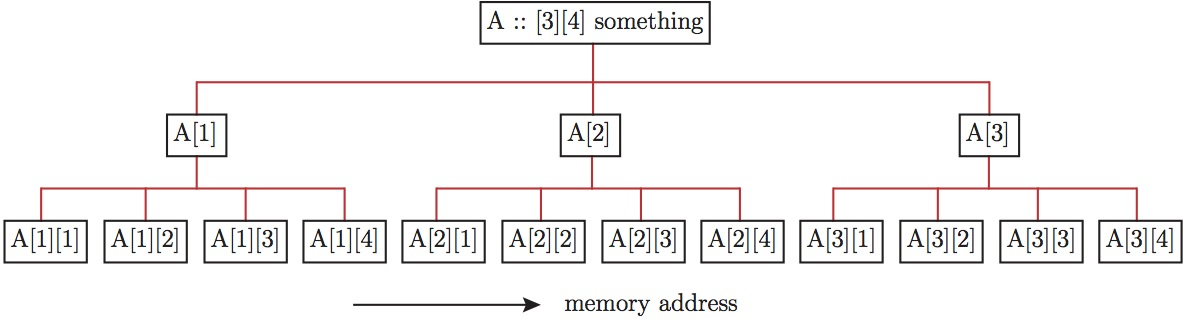
\includegraphics[width=\textwidth]{arrays}
\caption{Order of elements in a 2-dimensional array `\texttt{A}'}
\label{arrayElementOrder}
\end{figure}

When we address part of an array using two or more \verb#[*]# operators, Cicada loses track of how many elements were in each dimension and pretends that it is looking at a one-dimensional list.  For example, if we define:

\begin{code} \begin{verbatim}
grid :: [5][5] int
\end{verbatim} \end{code}

\noindent then both \verb#grid# and \verb#grid[*]# refer to a 2-dimensional array, but \verb#grid[*][*]# is effectively a single 1-dimensional list of 25 elements.  This is another technical limitation of Cicada, and it may change in the future.



\subsubsection{Resizing arrays (and composite variables)} \index{arrays!resizing|(}

All arrays in Cicada that are not `jammed' may be resized, and there are a number of ways to accomplish this.  The most straightforward method is to use the modified index operator \verb#[^...]# which sets the size of a single dimension of the array, as in

\begin{code} \begin{verbatim}
coordinates[^9]
\end{verbatim} \end{code}

\noindent The effect can be either to increase or reduce the size of the array.

Another way to resize an array is to use the all-indices operator \verb#[]# or \verb#*# for the \emph{last dimension} of an array that is being copied to.  The last dimension of the array will be resized only if necessary to prevent a mismatched-indices error.  So

\begin{code} \begin{verbatim}
numDays[*] = coordinates[*].x
\end{verbatim} \end{code}

\noindent should always work, whereas

\begin{code} \begin{verbatim}
numDays[<1, 5>] = coordinates[*].x
\end{verbatim} \end{code}

\noindent will only work if \verb#coordinates# has 5 elements.

Finally, we can insert an array index somewhere in the middle of an array using the \verb#[+...]# operator, or the \verb#[+<..., ...>]# operator for multiple indices.  We can also delete array indices using either the \verb#[-...]#/\verb#[-<..., ...>]# operators or the \verb#remove# command.  Here are some examples:

\begin{code} \begin{verbatim}
myArray[+5]                      | insert a new element before index 5
myArray[+<3, 6>]                 | insert 4 new elements before index 3
myArray[+<top+1, top+9>] = 17    | add 9 new elements at the end, and set them all to 17

myArray[-13]                     | delete array element #13
myArray[-<2, 4>]                 | delete array elements 2, 3 and 4
remove myArray[<2, 4>]           | same -- nix elements 2, 3 and 4
\end{verbatim} \end{code}

\noindent New array elements are always initialized in the same way as new arrays are:  for example if it is a numeric array the new elements are set to zero.

All of the operators for accessing, adding and deleting array elements also work on composite variables.  The difference is that, with composite variables, these operators access, add or delete members instead of array elements.  For example, if we define

\begin{code} \begin{verbatim}
threeNums :: {
    a := 2
    b := 5
    c := pi
}
\end{verbatim} \end{code}

\noindent then \verb#threeNums.b# is the same as \verb#threeNums[2]#.  If we want to delete the third member we can type either \verb#remove threeNums.c# or \verb#remove threeNums[3]#.  And we can add two members \emph{between} \verb#a# and \verb#b# by typing \verb#threeNums[+<2, 3>]#.  Those two new members will have no name, and initially will also have no data (see the forthcoming section on the void).  If we enter `\verb#threeNums#' after all these operations Cicada will print \verb#{ 2, *, *, 5 }#, showing that \verb#threeNums.b# is now \verb#threeNums[4]#.  In contrast, the old way of adding an extra member, say by typing \verb#threeNums.d :: int#, sticks the new member \verb#d# at the end of \verb#threeNums#.

We can never reference multiple elements of a composite variable except when removing them.  So \verb#threeNums[<2, 3>]# is not allowed.  Again, the technical reason is the storage of these two members' data is not contiguous, because each member is stored separately,.\index{arrays!resizing|)}\index{arrays|)textbf}



\subsubsection{This and that}

\index{this@\texttt{this}|(textbf}At any point in a script there are several objects (variables or functions) that can be referenced using a built-in keyword.  The first of these special keywords is `\verb#this#'.  In most examples from this chapter \verb#this# refers to the workspace variable -- the top-level space where the user's variables live.  But when a function is running, `\verb#this#' refers to the function.  For example, if we define the function

\begin{code} \begin{verbatim}
f :: {  int; this = args, return this  }
\end{verbatim} \end{code}

\noindent and type f(5), our function will set its internal integer variable to 5 and return itself:  \verb#{ 5 }#.  In general `\verb#this#' is whatever object contains the code that is currently running.

Be warned that there are two situations where `\verb#this#' may not point where we expect.  1) If we use the \verb#this# variable inside \emph{any} curly braces, as in

\begin{code} \begin{verbatim}
myVar :: {
    a := 2
    b := 5
    c := this[1]
}
\end{verbatim} \end{code}

\noindent then it refers to what is inside the curly braces, not the workspace (so in this case \verb#c# will be set to 2).  2) If `\verb#this#' appears inside the arguments of a function call, then it refers to any function arguments we have already passed.  The reason is a bit more complicated and will be explained later, but for example if we write

\begin{code} \begin{verbatim}
f(2, 5, this[2])
\end{verbatim} \end{code}

\noindent then we are effectively calling \verb#f(2, 5, 5)#.  In some cases this can be annoying:  for example if we want to print the number of workspace variables by typing

\begin{code} \begin{verbatim}
print(top(this))    | won't work
\end{verbatim} \end{code}

\noindent we will instead print `\verb#1#' which is the number of arguments of the \verb#top()# function.  What we really want to do is back out 2 levels, first to the arguments of \verb#print()# and then to the workspace, by typing\index{this@\texttt{this}|)textbf}

\begin{code} \begin{verbatim}
print(top(parent.parent))
\end{verbatim} \end{code}

\noindent \index{parent@\texttt{parent}|(textbf}\verb#parent# is the second predefined keyword, and refers to the object in the search path just before \verb#this#.  A shorthand for \verb#parent# is a backslash character, so the last example could also have been written\index{parent@\texttt{parent}|)textbf}

\begin{code} \begin{verbatim}
print(top(\.\))
\end{verbatim} \end{code}

\index{that@\texttt{that}|(textbf}A third keyword which appears only to the right of an assignment operator (\verb#=# or \verb#<-#) is called `\verb#that#'.  In its proper context, `\verb#that#' refers to whatever was on the left side of the assignment operator.  It can be used to abbreviate cumbersome expressions such as

\begin{code} \begin{verbatim}
facts.num.N = facts.num.N * log(facts.num.N) + facts.num.N
\end{verbatim} \end{code}

\noindent with

\begin{code} \begin{verbatim}
facts.num.N = that * log(that) + that
\end{verbatim} \end{code}\index{that@\texttt{that}|)textbf}

\index{args@\texttt{args}|(textbf}The final keyword, called \verb#args#, refers to a function's arguments, which is almost always a composite variable.  Functions are explained in more detail later, but here's a quick example:

\begin{code} \begin{verbatim}
I :: {
    code
    return { args, args[2] }
}
\end{verbatim} \end{code}

\noindent If we type the command \verb#I(1, 2, 3)#, our function \verb#I# will return \verb#{ { 1, 2, 3 }, 2 }#.\index{args@\texttt{args}|)textbf}




\subsubsection{Aliases} \index{aliases|(textbf}

C has pointers; Cicada has \emph{aliases}.  An alias is a member that shares its data with some other member:  they lead to the same variable.  In Cicada a member and its alias are \emph{exactly} on he same terms:  Cicada doesn't even know which was the original member.

Here is how aliases are defined:

\begin{code} \begin{verbatim}
a := 2       | will default to an int
b :=@ a      | alias #1
c :=@ b      | alias #2
\end{verbatim} \end{code}

\noindent `\verb#b#' is now an alias to `\verb#a#', and `\verb#c#' is now an alias to `\verb#b#' and therefore also to `\verb#a#'.  If we were to now \texttt{print(a)}, \texttt{print(b)} or \texttt{print(c)}, we would get back the number 2.  If we were to set any of the three variables to a different value:

\begin{code} \begin{verbatim}
c = 3
\end{verbatim} \end{code}

\noindent then printing any of \texttt{a}, \texttt{b} or \texttt{c} would then cause the new number 3 to be printed.

Any variable can become an alias for any other variable \emph{of the same type} (or a derived/inherited type), by means of the equate-at operator `\texttt{=@}'.

\begin{code} \begin{verbatim}
a :: b :: c :: int
{ a, b, c } = { 1, 2, 3 }
a =@ b                | 'a' now points to the variable storing '2'
b =@ c                | 'a' STILL points to the variable storing '2'
c =@ b =@ a
\end{verbatim} \end{code}

\noindent The tricky bit is the fourth line:  since member `\verb#a#' has been aliased to member `\verb#b#', does the command \verb#b =@ c# now drag member \verb#a# along with it?  The answer is no:  aliasing binds one member to another member's variable, not to the other member itself.  If we follow through all the acrobatics, we find that members \verb#a#, \verb#b#, and \verb#c# all end up referring to same the variable storing the number 2, as shown in Figure \ref{aliases}.  (The other two variables are now inaccessible and will eventually be cleared from memory.)

\begin{figure}
\centering
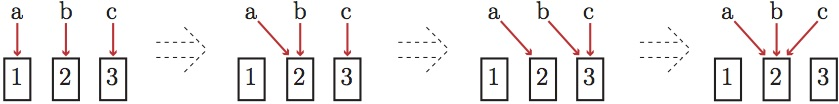
\includegraphics[width=\textwidth]{aliases}
\caption{Aliasing of members (letters) to variables (boxes)}
\label{aliases}
\end{figure}

Cicada clearly makes an important distinction between members and variables.  Until now we have been rather sloppy on this point, so we shall be more careful from now on.  A member\index{members|textbf} is a named object in Cicada:  the name of a variable, or a field in a composite variable.  The variable itself is the data that the member refers to.  In Cicada these two objects are entirely separate, and there is no reason to require a one-to-one correspondence between them.

Just as the data-copying operator `\verb#=#' or `\verb#<-#' has a data-comparison counterpart `\verb#==#', so the member-reference-copying operator `\verb#=@#'  is mirrored in a reference-comparison operator `\verb#==@#' which tests to see whether two members point to the same object.  (If the left side spans a range of array elements then the right side must also span exactly those same elements in order for the test to return true).  Finally, the is a reference-not-equal operator `\verb#/=@#' is just the logical negation of `\verb#==@#'.\\

If we so prefer, we can write whitespace just before the `@' of any of the aliasing operators.

\begin{code} \begin{verbatim}
if a == @b  then c := @b
if a /= @b  then a = @b
\end{verbatim} \end{code}

\noindent The extra space makes clearer the analogy with the data-copying operators:  both \verb#a = @b# and \verb#a = b# cause member `\verb#a#' to equal member `\verb#b#', though by different means.  By the way an \texttt{@} symbol by itself is meaningless; it is only the last character of these aliasing operators.\index{aliases|)textbf}



\paragraph{Jamming} \index{arrays!jamming|(}

Arrays can also be involved in aliasing.  There is a potential complication, but on the surface it is straightforward.  For example, we ordinary (non-array) members can alias single array elements.

\begin{code} \begin{verbatim}
array_1 :: [5] double
array_2 :: [10] double
oneEl :: double

oneEl = @array_1[4]
oneEl = @array_2[top]
\end{verbatim} \end{code}

\noindent Likewise \emph{complete} arrays can alias other arrays, or parts of larger arrays.  (Cicada doesn't let us re-alias just \emph{some} indices of an array since that would fragment its memory.).  So we can write

\begin{code} \begin{verbatim}
array_1[*] = @array_2[<4, 8>]
\end{verbatim} \end{code}

\noindent but \emph{not}

\begin{code} \begin{verbatim}
array_1[<3, 5>] = @array_2[<4, 6>]
\end{verbatim} \end{code}

The complication is that arrays having multiple members pointing to them can become `jammed', meaning that they cannot be resized.  The reason is that resizing one of its members would also force a resize of the other member which may be in an unrelated part of code, and this is not allowed.  Here is an example.

\begin{code} \begin{verbatim}
array_1 :: [3][10] int
array_2 := @array_1[2][<4, 7>]   | jams 4 indices of array_1

array_1[*][^12]        | legal
array_2[^12]           | no, this would cause problems
remove array_1[*][5]   | not legal
remove array_1[1]      | legal

remove array_1
array_2[+3]            | legal only because we removed the jamb
\end{verbatim} \end{code}

Explicit aliases always jam arrays.\index{aliases}  On the other hand, unnamed references to objects (such as elements of sets and function arguments) never jam arrays.

\begin{code} \begin{verbatim}
al := @my_array[<4, 6>]    | jams elements 4-6
my_array[<4, 6>]                 | does not jam
\end{verbatim} \end{code}

\noindent Tokens\index{tokens} are `unjammable', both in the sense that they cannot jam, and that they will become `unjammed'---i.e. permanently deactivated---if their referent is resized through another member.  An unjammed token becomes unusable until it is redefined (when happens when the line defining the token is rerun).\index{arrays!jamming|)}





\subsubsection{The void}

\index{nothing@\texttt{nothing}|(textbf}\index{void, the|see{nothing}}There is one last way to define a variable, and that is not to define it as anything at all.  There are two ways of writing this:

\begin{code} \begin{verbatim}
var1 :: nothing
var2 :: *
\end{verbatim} \end{code}

\noindent \verb#nothing# and \verb#*# are synonyms for the void operator.  If \verb#var1# is defined as void then we will get a void-member error if we try to access its data.  In fact, one of the few things we can do with a void member is to test whether it is void or not, using the reference-comparison operator \verb#==@#.

\begin{code} \begin{verbatim}
if var1 == @nothing  then &
    print("out of order..\n")
\end{verbatim} \end{code}

One way to make use of a void member is to redefine it.

\begin{code} \begin{verbatim}
var1 :: nothing
var1 :: [1000] string
\end{verbatim} \end{code}

\noindent We could have redefined \verb#var1# as anything:  a primitive or composite variable, function, etc.  But once it's been redefined once \verb#var1# cannot be redefined again except to the same type or a derived type (see inheritance).

What is the use of defining void-typed variables (aside from the fact that they don't take up space until we redefine them)?  The main reason is that 1) members defined this way have no type (unless you redefine them), and 2) members without a type can alias any other member, because in a sense all data types are derived from the void.  This works as long as we don't redefine the alias (i.e. we have to just use the \verb#=@# operator, not \verb#:=@#).

\begin{code} \begin{verbatim}
any_var :: *
x :: int
y := "some string"
z :: { double, int }

any_var = @x
any_var = @y
any_var = @nothing
any_var = @z
\end{verbatim} \end{code}

The fact that the void is the universal parent type also explains why void members can be redefined.  Cicada always permits an existing member's type to be specialized---restricted to a subtype of its original type---but never changed to an unrelated type.  And we cannot un-specialize:  an \verb#int# member cannot be turned it back into \verb#nothing#, except by removing and reallocating the member.

There are actually two uses of the word `void' in this document that are important to keep logically separate.  A void member is one that has no storage space.  But a void-\emph{typed} member is one with essentially no type restriction on what it can point to.  A definition like \verb#a :: *# does \emph{two} things:  it defines a member `\verb#a#' having no type, and it therefore neglects to give `\verb#a#' any storage space.

Cicada also distinguishes between member types and variable types.  For example, after \texttt{any\_var} was aliased to \texttt{x}, did \texttt{any\_var} have a null type or was it an \verb#int#?  Well, that depends on whether you are asking about the member's type (which was void), or the type of the variable it points to (an integer).  Both members and variables have types, and in general (as in the example above) they may be different.  A member's type specification\index{members!type|(} determines which variables it is allowed to point to.  The rule is that a member can only target variables with the same type, or having a sub-type derived from its own.  The only exception is that members of any type can be aliased to `\texttt{*}', but the void hardly qualifies as a normal variable.\\




\subsection{Other define and equate operators}

The difference between a member's type and the type of its target variable motivates two further define operators.

The variable-define operator `\texttt{@::}' is identical to ordinary define (\texttt{::}), except that it only sets the target variable's type, while leaving the member's type unchanged.  That means that if it is used to define a brand new member, that member's type will be void.  For example, here we use this operator to define and then redefine a member with different types of storage, and then alias it to another variable of a different type.

\begin{code} \begin{verbatim}
theVar @:: int
...
theVar = @nothing    | need to unlink before creating a new variable
theVar @:: string
...
theBool :: bool
theVar = @theBool
\end{verbatim} \end{code}

\noindent Notice that the second \verb#@::# operator was forced to make a new variable because \verb#theVar# had been unlinked (aliased to the void) on the previous line.  Had we left out the unlinking command, Cicada would have tried to redefine the existing \verb#int# \emph{variable} as a \verb#string#, causing a type-mismatch error.

The member-define operator `\texttt{*::}' is the counterpart to variable-define:  it only acts upon the member, without affecting any variable that member may target.  Its symbol reflects the fact that, if one uses member-define to define a new member, it will indeed create a member of the desired type but it will not bother to create a variable for it, so the member will point (be aliased) into the void.  So the following code will cause an error:

\begin{code} \begin{verbatim}
myNum *:: int
myNum = 5      | will cause an error
\end{verbatim} \end{code}

\noindent which could have been avoided had we written \verb#myNum :: int# or \verb#myNum @:: int# between the two lines, in order to construct the variable behind the member.  But it has to be an integer variable, in order to be compatible with member \verb#myNum#'s type.\index{nothing@\texttt{nothing}|)textbf}\index{members!type|)}

There are actually 256 operators in the define family, most of which cannot be scripted directly unless we modify the language.  See Chapter 4.\\

Finally, there is another assignment operator called `forced-equate', and given the symbol `\texttt{=!}' or `\verb#<-!#'.  While equate copies data between variables whose data structures match or are compatible (e.g. \verb#{ int, string }# to \verb#{ double, string }#), forced equate copies between variables having the same memory storage size.  (Having a string in the destination variable makes the storage requirement somewhat elastic.)  A forced equate simply takes the data contained in its right-hand argument and stuffs those $N$ bytes in the same order into the left-hand variable, with no restrictions on how the storage space is parceled out within the destination variable.

When forcing an equate from an inlined numeric constant, remember that Cicada interprets constants as either as signed long integers or floating-point doubles, according to the convention described in the earlier section on expressions.  So on the author's old machine where long integers are 4 bytes and doubles are 8 bytes, \verb@a =! -4@ and \verb@a =! 2e5@ will copy 4 bytes while \verb@a =! 4.@ and \verb@a =! 2e10@ will each copy 8 bytes.

Here are some examples showing the difference between these two operators:

\begin{code} \begin{verbatim}
var1 :: { int, bool }
var2 :: { double, bool }
var3 :: { int, string }

var1 = var2    | OK
var1 = var3    | type-mismatch error

var1 =! var2   | unequal data size error
var1 =! var3   | unequal data size error unless string has 1 character
var3 =! var1   | OK, surprisingly!
\end{verbatim} \end{code}

\noindent The last line works because forced-equate resizes \verb#var3#'s string as needed to soak up any extra bytes from \verb#var1#.




% --------------- Flow control --------------


\subsection{Loops and \texttt{if} blocks} \index{flow control|(}

Cicada has four commands for controlling the program flow:  \texttt{if} statements, \texttt{for} loops, and \texttt{while} and the related \texttt{do} loops.


\subsubsection{\texttt{if}} \index{if@\texttt{if}|(}

There are several differences in syntax between an \texttt{if} statement in Cicada and one in C.  Firstly, the logical test is between the \verb#if# and a \verb#then# keyword, rather than being inside parentheses.

\begin{code} \begin{verbatim}
if a == b  then print("They're equal.\n")
\end{verbatim} \end{code}

\noindent Secondly, some of the logical operators are different.  `\verb#and#'\index{and@\texttt{and}}, `\verb#or#'\index{or@\texttt{or}}, `\verb#xor#'\index{xor@\texttt{xor}} and `\verb#not#'\index{not@\texttt{not}} are all written out in words, and the is-not-equal operator is \verb#/=#, not \verb#!=#.  Cicada also has the reference-comparison operators `\verb#== @#' and `\verb#/= @#' (see \emph{aliases}).

\begin{code} \begin{verbatim}
if a == @nothing and b /= @nothing  then print("a, but not b, is void.")
\end{verbatim} \end{code}

\noindent Third, since the entire \verb#if# statement is one single command and (unlike in C) a line break \emph{ends} commands, if we want to break it over several lines we need to either use a `\verb#&#' which continues lines, or else parentheses \emph{beginning on the line} of the \verb#if# statement.

\begin{code} \begin{verbatim}
if a == b  then &
    print("They're equal.\n")

else if a /= b  then (
    print("They're different.\n")
)
\end{verbatim} \end{code}

\noindent Finally, the latter method shows how to write multi-line \verb#if# statements:  using parentheses instead of curly braces.  (Technical note:  while curly braces actually work for most \verb#if# statements, they also produce a new variable space, so defining new members or using the keyword \verb#this# won't do what you expect.  Just use parentheses.)

\begin{code} \begin{verbatim}
if a /= @nothing and b /= @nothing  then (       | avoid a crash
    if a == @b  then print("They're the same variable!\n")
    else if a == b  then print("They're equal.\n")
    else  print("They're different.\n")      )

else  print("At least one of these members is VOID!")
\end{verbatim} \end{code}

\index{if@\texttt{if}|)}



\subsubsection{\texttt{while do} and \texttt{loop until}} \index{while@\texttt{while}|(} \index{loop@\texttt{loop}|(} \index{until@\texttt{until}|(}

Cicada's \verb#while...do# loop is pretty similar to C's \verb#while# loop, except that the logical condition goes between the \verb#while# keyword and a \verb#do# keyword instead of inside parentheses.  Also, the logical operators are somewhat different and we use parentheses to group multi-line commands, in the same way as with the \texttt{if} statement.

\begin{code} \begin{verbatim}
while input() /= "pleeez"  do print("what's the magic word?  ")
while input() == "thank you"  do (
    print("you are welcome!\n")
    print("anything else?  ")
)
\end{verbatim} \end{code}

There are two differences between Cicada's \texttt{loop} loop and its \verb#while# loop.  First, the break condition of a \texttt{loop} loop is evaluated at the end of the loop, so it always runs at least once.  Second, it is a \verb#loop...until# loop, not a \verb#loop...while# loop, so it keeps looping as long as the logical condition is \emph{not} satisfied.

\begin{code} \begin{verbatim}
attempt := 0
loop  (
    print("Thank you!\n")
    attempt = attempt+1
)  until input() == "you're welcome"

loop print("> ") until input() == "exit"
\end{verbatim} \end{code}

\index{while@\texttt{while}|)}\index{loop@\texttt{loop}|)}\index{until@\texttt{until}|)}



\subsubsection{\texttt{for}} \index{for@\texttt{for}|(}

Cicada's \texttt{for} loop is simpler and offers less control than C's.  Here is an example showing the syntax.

\begin{code} \begin{verbatim}
counter :: int
for counter in <1, 10-counter>  print(counter, " ")
\end{verbatim} \end{code}

\noindent Notice that we had to define the loop variable before the loop, as either an \verb#int# or a \verb#double#.  The loop itself will print the numbers 1 through 5; when \verb#counter# reaches 6 it will be greater than \verb#10-counter# and the loop will stop.

As always, we can break a loop over two lines using a `\verb#&#', and we can group several lines of code using parentheses beginning on the line of the \verb#for# command.  So we could have rewritten our code above in several different ways.

\begin{code} \begin{verbatim}
counter :: int

for counter in <1, 10-counter>  &
    print(counter, " ")

for counter in <1, 10-counter>  (
    print(counter)
    print(" ")
)
\end{verbatim} \end{code}

Unlike Cicada's predecessor (Yazoo scripting language) there is no \verb#step# argument to control the increment of the counter variable.  This is due to limitations of the new compiler.  Of course there are a number of ways around this, one of which is to change the loop to a \verb#while# loop and do the step manually.  The loop in our example is equivalent to:

\begin{code} \begin{verbatim}
counter := 1
while counter <= 10-counter  do (
    print(counter, " ")
    counter = that + 1
)
\end{verbatim} \end{code}

\index{for@\texttt{for}|)}



\subsubsection{\texttt{break}} \index{break equivalent|(}

There is no \verb#break# statement in Cicada.  But there is a way to jerry-rig something that does pretty much the same.  The trick is to put braces -- with no \verb#code# marker or semicolon -- around the code we eventually want to escape from.  Within those braces, a \verb#return# statement will simply escape from the bracketed code and continue with what follows.  For example:

\begin{code} \begin{verbatim}
{
    for counter in <1, 10>  (
        print(counter)
        if input() == "q"  then return    )
}
print("finished with counter = ", counter)
\end{verbatim} \end{code}

\noindent This works because the braces actually define a new composite variable, and the code inside the braces is actually running inside of this variable.  This causes problems in some cases.  If we define a member, that member will be inside of this variable, which was probably not intended.  The \verb#this# keyword refers to this newly-defined variable, while \verb#parent# now refers to the place we were before hitting the braces.  Also, if we had been running a function, we cannot escape this function using a \verb#return# statement within the bracketed code.  On the upside, we have a lot of latitude in choosing where to put the braces:  it doesn't have to escape from a loop, and if we do use them inside loops it does not have to be to the next-outermost \verb#for# or \verb#while#.\index{break equivalent|)}

\index{flow control|)}





% -----------------  Sets  ----------------


\subsection{Sets} \index{sets|(}

One object in Cicada that is not supported by C is the \emph{set}.  A set is like a bag of assorted objects---variables, functions, classes, even other sets---that are exist somewhere else except that they can also be found, magically, by reaching into the bag.  To define a set we write curly braces around a list of objects separated by commas (or end-of-lines).  Here is an example where each object is in several places.

\begin{code} \begin{verbatim}
Alice :: Bob :: Christine :: Daniel :: Elan :: friend_of_mine

men :: { Daniel, Elan, Bob }
neighbors :: { Christine, Bob }
cleaning_schedule :: { Bob, Alice, Bob, Alice, Elan, Elan, Daniel }
\end{verbatim} \end{code}

\noindent We typically access members of a set using square brackets (as if they were arrays).  So after running the code, \texttt{Bob}, \texttt{men[3]}, \texttt{neighbors[2]}, \texttt{cleaning\_schedule[1]} and \texttt{cleaning\_schedule[3]} are all the same thing.  If we set \verb#men[3].needsSleep = true# then \verb#Bob.needsSleep# and \verb#neighbors[2].needsSleep# will also be \verb#true#.  Notice how the same object can even appear in several places in a set.  Sets come handy when the objects have convoluted path names.

\begin{code} \begin{verbatim}
to_buy :: {
    food.produce.fruits.apples
    clothes.shoes.black
    clothes.socks.black
}
\end{verbatim} \end{code}

\noindent \verb#to_buy[1]# is much quicker than \texttt{food.produce.fruits.apples}.

Cicada sets are pretty flexible in what they can store.  Along with variables, we can throw constants, other sets (including ones that we define on the fly), and even the void into the bag.

\begin{code} \begin{verbatim}
collections :: { men, neighbors, { Patty, Don }, "Herbert", 3.3, this[3], this, nothing }
\end{verbatim} \end{code}

\noindent Here \verb#collections[3]# is an inlined subset containing two objects.  The fourth and fifth items are inlined constants.  The \verb#collections[6]# \emph{is} also the third item, the subset containing \verb#Patty# and \verb#Don#, and notice that it had to be listed after the third item because otherwise \texttt{this[3]} would not have existed yet.  \verb#collections[7]# is \verb#collections# itself -- so \verb#collections[7][7][7][2]# is just \verb#neighbors#.  Trying to print \verb#collections# from the command line won't work because of the self reference.

The reason we access set elements by their index (as opposed to name) is that those set elements \emph{have no name}, at least the way we defined them in our examples.  In other words, \verb#collections[1]# is effectively an alias for \verb#men# but that doesn't mean that that set element has the name \verb#men# -- \texttt{collection.men} will cause Cicada to draw a blank.  But there is actually a way to name certain elements of a set, and that is to manually define aliases for their respective objects.  To illustrate, here we give a different way of defining \texttt{collections} which assigns names to members 2, 3, 4, 7 and 8.

\begin{code} \begin{verbatim}
collections :: {
    men
    neighbors := @parent.neighbors      | use same name for convenience
    peeps :: { Patty, Don }
    Herby := "Herbert"
    3.3,  this[3]          | set elements 5 and 6
    myself := @this
    zilch := @nothing
}
\end{verbatim} \end{code}

\noindent With the verbose definition we can write \texttt{collections.Herby} in place of \texttt{collections[4]}, although \texttt{collections[4]} is still perfectly legal.

Just as with composite variables, items can be added to and removed from sets after they have been defined.  So if we want to shuffle ``\texttt{Herbert}'' to the end of the set we might write:

\begin{code} \begin{verbatim}
collections[top+1] := @collections.Herby
remove collections.Herby
\end{verbatim} \end{code}

\noindent (and those 2 lines could go in any order).

As with variables, we can use one set to define another.  The following is legal:

\begin{code} \begin{verbatim}
newCollections :: collections
\end{verbatim} \end{code}

\noindent Importantly, \verb#newCollections# is defined using the old set \verb#collections#'s \emph{original} definition.  So even if we had rearranged the elements of \verb#collections#, in the new set \verb#Herbert# will be both at \verb#newCollections[4]# and \verb#newCollections.Herby#.  We might as well have defined both sets on the same line:

\begin{code} \begin{verbatim}
newCollections :: collections :: { ... }
\end{verbatim} \end{code}


\index{sets|)}






% -----------------  Functions  ----------------


\subsection{Functions} \index{functions|(}

A basic Cicada function call looks exactly the same as a C function call.

\begin{code} \begin{verbatim}
y = f(x)
\end{verbatim} \end{code}

\noindent But behind the familiar syntax roams what is probably the strangest beast in all the Cicada language.  For one thing, Cicada functions are \emph{objects} that live in ordinary heap memory, unlike their stack-dwelling counterparts in C.  Cicada functions have no input type and no output type, and they can have several coding sections.  Function arguments are hopelessly different between the two languages.  These changes together allow Cicada functions to be used in some unusual ways.



% -----------------  Function definitions  ----------------

\subsubsection{Defining functions (properly)}

Cicada functions are \emph{objects}, like composite variables and sets (the analogy here is closer than you would think).  So we define functions using the same operators we use for defining other objects.  The function code goes inside curly braces beginning on the line of the definition.  Here is an example.

\begin{code} \begin{verbatim}
SwapDigits :: {
    
    tensDigit :: onesDigit :: int
    
    code
    
    tensDigit = floor(args[1] / 10)
    onesDigit = args[1] mod 10
    
    return new(10*onesDigit + tensDigit)
}
\end{verbatim} \end{code}

\noindent The function shows us several new keywords.  1) A `\texttt{code}'\index{code@\texttt{code} marker|textbf} marker (or semicolon) separates the function's variable definitions from its executable code.  Before the \verb#code# marker, the function's internal variables are defined in exactly the same way as global variables in the workspace are defined.  2) Function arguments are contained inside of an \texttt{args}\index{args@\texttt{args}} variable, and we access them using the index operators \verb#[]#.  The function exits with the classic \texttt{return}\index{return@\texttt{return}} statement, just as in C except 3) we enclosed the return value inside of a \verb#new()# function call.

Once we have written the function, we can run it in the normal way.

\begin{code} \begin{verbatim}
> print(SwapDigits(27))

72
\end{verbatim} \end{code}

\noindent From the command line we can also just type the function name and read off the output:

\begin{code} \begin{verbatim}
> SwapDigits(27)

72
\end{verbatim} \end{code}

\noindent Sometimes the automatic output can be annoying:  the function may be performing an important task but we don't care about the return value.  To throw away the return value, append a `$\sim$' operator to the function call:  \texttt{SwapDigits(27)}$\sim$.

In Cicada we can treat functions as if they were variables, peek at all their internal members, and even fiddle around inside them.  This is useful for debugging.

\begin{code} \begin{verbatim}
> SwapDigits.tensDigit            | did it do what we wanted?

2

> remove SwapDigits.onesDigit     |  let's see if it still works..
\end{verbatim} \end{code}

Finally, functions can define other functions:

\begin{code} \begin{verbatim}
> SD2 :: SwapDigits
\end{verbatim} \end{code}

\noindent We broke \verb#SwapDigits()# when we deleted its \verb#oneDigit# member, but \verb#SD2# is defined using the \emph{original definition} of \verb#SwapDigits# so it will work just fine.

One situation that requires several copies of a function is recursion\index{recursion|(}.  This is because each nested recursive instance of the function requires its own storage.  This is true whether a function \verb#f()# calls itself directly or indirectly (\verb#f()# calls \verb#g()# calls \verb#f()#).  Here is an example that handles recursion properly.

\begin{code} \begin{verbatim}
factorial :: {
    
    numToReturn :: int
    
    code
    
    if args[1] == 1  then numToReturn = 1
    else  numToReturn = args[1] * (new_fact :: this)(args[1]-1)
    
    return numToReturn
}
\end{verbatim} \end{code}

\noindent Importantly, the definition \verb#new_fact :: this# had to be in the \emph{coding section} of \verb#factorial()#.  If we had put the definition \verb#new_fact()# \emph{before} the \verb#code# marker, \verb#factorial.new_fact# would have defined another member \verb#factorial.new_fact.new_fact#, etc. until Cicada threw in the towel with a recursion-depth error.\index{recursion|)}

Our last example might have handled recursion correctly, but it did something else quite wrong, as we find out by typing

\begin{code} \begin{verbatim}
> { factorial(3), factorial(4) }

{ 24, 24 }
\end{verbatim} \end{code}

\noindent The second call to \verb#factorial()# overwrote the first!  The reason is that our set consists of two aliases to \verb#numToReturn#, whose value changes with each function call.  The solution is to have \verb#factorial()# redefine \verb#numToReturn# each time it is run.\index{new@\texttt{new()}|(}

\begin{code} \begin{verbatim}
    return new(numToReturn)
\end{verbatim} \end{code}

\noindent The \verb#new()# function is defined in \verb#user.cicada# which pre-loads when Cicada is run interactively.\index{new@\texttt{new()}|)}  If \verb#user.cicada# wasn't loaded we have to redefine our return variable manually.

\begin{code} \begin{verbatim}
factorial :: {
    
    numToReturn :: int
    
    code
    
    (numToReturn =@ *) :: int        | redefining an unlinked member creates a new variable
    
    if args[1] == 1  then numToReturn = 1
    else  numToReturn = args[1] * (new_fact :: this)(args[1]-1)
    
    return numToReturn
}
\end{verbatim} \end{code}

Here is one unusual feature\index{code number operator|(} of Cicada functions:

\begin{code} \begin{verbatim}
f :: {
    num := 2
    
    code
    num = that + 1
    
    code
    return num   }
\end{verbatim} \end{code}

\noindent Two coding blocks---so there should be a way to access them both.

\begin{code} \begin{verbatim}
> f()


> f#2()

3
\end{verbatim} \end{code}

\noindent The code-number operator `\verb$#$' lets us run the code beginning at the $N$th \verb#code# marker.  By running \verb$f()$, which defaults to \verb$f#1()$, we incremented \verb#f.num#.  But execution stopped at the next \verb#code# marker.  There was no \verb#return# statement, which is fine:  the function returns \verb#nothing#, just as it would had we written \verb#return# or \verb#return *#.  In order to get a value back we had to run the \emph{second} coding block which returned \verb#f.num#.  Incidentally, had we run \verb$f#0()$ we would rerun \verb#f#'s `constructor' and find \verb#f.num# reset to 2.\index{code number operator|)}

Short functions like \verb#f()# are sometimes easier to code on one line.  To do this we use the fact that commas are equivalent to ends-of-lines, and semicolons are equivalent to \verb#code# markers.

\begin{code} \begin{verbatim}
> f :: {  num := 2; num = that + 1; return num  }
\end{verbatim} \end{code}







% -----------------  Function arguments  ----------------

\subsubsection{Function arguments} \index{functions!arguments to|(}

Notice that the definition of a Cicada function doesn't specify any argument list.  That means functions in Cicada are automatically able to handle different argument types, variable numbers of arguments, etc.  Here is a simple function that can take any arguments whatsoever, as long as there are at least 2 of them.

\begin{code} \begin{verbatim}
> arg2 :: {  code, return args[2]  }


> arg2(5, 3+9, 'C')                             | return a number

12

> arg2(pi, { a := 3, b := 4; return a*b })      | return a function! 

{ 3, 4 }
\end{verbatim} \end{code}

\noindent Cicada functions also don't specify return types, and as our last example shows a single function can return different kinds of values even from the same \verb#return# statement.  And of course different \verb#return# statements within the same function can return different types of objects.\\

\index{args@\texttt{args}|(textbf}What happens if we stick a \texttt{code}\index{code@\texttt{code} marker} marker (or semicolon) \emph{inside the function's argument list}?  When we try this experiment, we'll find out is that anything after the function arguments' \verb#code# marker isn't created, or doesn't run, until the function \emph{runs its arguments}.

\begin{code} \begin{verbatim}
PrintArgs :: {
    code
    
    print("Before running args:  ", args, "\n")
    args()
    print("Afterwards:  ", args, "\n")
}
\end{verbatim} \end{code}

\noindent If we call

\begin{code} \begin{verbatim}
PrintArgs( 0.3, " 4", code, " word ", 10 )
\end{verbatim} \end{code}

\noindent then the function prints

\begin{code} \begin{verbatim}
Before running args:  0.3 4
Afterwards:  0.3 4 word 10
\end{verbatim} \end{code}

\noindent We can even put coding statements in the function arguments.

\begin{code} \begin{verbatim}
PrintArgs( " *** announcement *** ", code, print("I am an argument list.\n") )
\end{verbatim} \end{code}

\noindent which causes the output

\begin{code} \begin{verbatim}
Before running args:  *** announcement *** 
I am an argument list.
Afterwards: *** announcement *** 
\end{verbatim} \end{code}

\noindent In fact an argument list can run any code whatsoever.  A few tricky points:  if we define variables, etc. inside of an argument list then they will only exist inside that function's \verb#args# variable; \verb#this# inside the argument list refers to \verb#args#, not the variable space where the function was called (that will be \verb#parent#); and \verb#return# inside of \verb#args# only stops execution of \verb#args#'s code.

If we can \emph{run} the \texttt{args} list, surely we can also pass it parameters?  Write a new function to test this:

\begin{code} \begin{verbatim}
> doArgs :: {  code, args(9, "lives"), return args  }


> doArgs( args, code, print(top(args), " arguments were passed\n") )

2 arguments were passed
{ {  } }
\end{verbatim} \end{code}

\noindent This example is complicated, particularly the function call (2nd command entered at the prompt).  On this line, within the parentheses, `\texttt{args}' refers to two different things depending on which side of the \verb#code# marker it falls on.  Before the \verb#code# marker, \verb#args# holds the same value it had when the function was called, except wrapped in a second layer of curly braces.  But \emph{after} the \verb#code# marker, `\texttt{args}' was the parameter list that ran \texttt{doArgs} passed to its arguments, containing the number 9 and the string \verb#"lives"#.  Each function call temporarily replaces the existing \verb#args# variable with its own argument list; the old \verb#args# comes back when each function exits.

Here's another example showing more explicitly how \texttt{args} changes across the \texttt{code} marker.

\begin{code} \begin{verbatim}
f :: {
    code
    
    g( print(args, " --> "), code, print(args) )
}

g :: {  code, args("B")  }
\end{verbatim} \end{code}

\noindent That is, \texttt{f()} runs \texttt{g()}, which in turn runs its own arguments.  Now run \verb#f()#.

\begin{code} \begin{verbatim}
> f("A")

A --> B
\end{verbatim} \end{code}

\noindent Focus on the line in which function \verb#f()# calls function \verb#g()#.  The part of \verb#args# \emph{before} the \verb#code# marker is built before \verb#g()# is run, so here \texttt{args} still has its old value `\texttt{A}'.  The part of \verb#args# \emph{after} the \verb#code# marker is called by \texttt{g()}, so here \texttt{args} is `\texttt{B}'.

Finally, function arguments can contain \verb#return# statements just like normal functions.

\begin{code} \begin{verbatim}
> doTwice :: {  num :: double, code, num = args[1], return args(args(num))  }


> doTwice(3, code, return new(args[1]^2))        | calculate (3^2)^2

81
\end{verbatim} \end{code}

To summarize, Cicada's function arguments are themselves functions.  If the syntax for function calls were not so standardized the author would have chosen curly braces, so imagine:

\begin{code} \begin{verbatim}
***  doTwice{ 3, code, return new(args[1]^2) }  ***
\end{verbatim} \end{code}

\noindent This way of writing a function makes it clear how the arguments are just some function object that's ordinarily invisible, but appears as \verb#args# when we run \verb#doTwice()#.  This syntax is not legal by the way --- but if you want to allow it, just duplicate the line defining function calls in \verb#cicada.c# and change the parentheses to curly braces.

\index{args@\texttt{args}|)} \index{functions!arguments to|)}




% -----------------  Code substitution  ----------------

\subsubsection{Code substitution}

Why would a function ever want to run its arguments?  One good reason is that an \verb#args()# call is the easiest way for a function to accept optional parameters.  To do this, we must write the function so that all of its optional parameters (or aliases to them) are grouped into one composite variable.  When the function is called, it will first set those parameters to their default values, then run \verb#args()# \emph{inside of the parameters variable} with the help of the code substitution operator `\verb#<<#'.  Here is an example.

\begin{code} \begin{verbatim}
RollDice :: {
    
    numDice :: total :: loopDie :: int
    
    params :: {
        numSides :: int
        isLoaded :: bool    }
    
    code
    
    { numDice } = args
    
    params = { 6, false }
    (params << args)()
    ...
}
\end{verbatim} \end{code}

\noindent If we are happy with the default values of \verb#numSides# and \verb#isLoaded#, so we can leave them out.

\begin{code} \begin{verbatim}
RollDice(5)
\end{verbatim} \end{code}

\noindent The function call only needs a coding section when we want to cheat or roll exotic dice.

\begin{code} \begin{verbatim}
RollDice(5; isLoaded = true)
\end{verbatim} \end{code}

All members of \verb#params# must be explicitly named.  This would be an \emph{incorrect} definition:

\begin{code} \begin{verbatim}
    numSides :: int
    isLoaded :: bool
    
    params :: { numSides, isLoaded }
\end{verbatim} \end{code}

\noindent The problem is that neither member of \verb#params# has a name, so a function call can't easily change it.  A member aliasing the \verb#isLoaded# variable is not the same as a member named \verb#isLoaded#.\\


In general, a code substitution \verb#D << F#, involving composite variables or functions \verb#D# and \verb#F#, returns the data space of \verb#D# along with the code of \verb#F#.  On the other hand, plain \verb#F# returns both the data space and the code of \verb#F#.  The two basic properties of composite variables and functions are data and code, and the code substitution operator is the tool for separating and recombining these properties.

There are many uses for code substitution beyond optional function arguments.  For example, \verb#start.cicada# uses it to run the user's commands inside of the workspace variable.  Code substitution can save a lot of typing when working with awkward pathnames.  For example, instead of

\begin{code} \begin{verbatim}
games.backgammon.RollDice.params.numSides = 20
games.backgammon.RollDice.params.isLoaded = true
games.backgammon.RollDice.params.dieColor := "green"
...
\end{verbatim} \end{code}

\noindent we can just write

\begin{code} \begin{verbatim}
(games.backgammon.RollDice.params << {
    
    code
    
    numSides = 20
    isLoaded = true
    dieColor := "green"
    ...
})()
\end{verbatim} \end{code}

\noindent Notice that we had to write all of our commands after a \texttt{code} marker, and run the substituted code as a function.  That way the assignment commands will run inside of the \verb#params# variable.

A code substitution is quite temporary:  it only lasts as long as the immediate expression is being evaluated.  The next time we run \verb#RollDice()# it will be its normal self, except that its \verb#params# variable will have a new member \verb#dieColor#.

The code-number\index{code number operator|(} operator can be used to control which code is passed to the code-substitution operator.  Here is a function that uses either one or two sets of optional parameters, depending on how it is called.

\begin{code} \begin{verbatim}
f :: {
    ...
    
    code
    
    params_1 :: { doMoreStuff := false, ... }
    params_2 :: { otherNum :: int, ... }
    
    (params_1 << args)()
    if params_1.doMoreStuff  then (params_2 << args#2)()
    
    ...
}
\end{verbatim} \end{code}

\noindent When we call this function, our arguments will contain 1, 2 or 3 coding blocks.

\begin{code} \begin{verbatim}
f(2, 5)                                             | don't doMoreStuff
f(2, 5; doMoreStuff = true)                         | doMoreStuff w/ defaults
f(2, 5; doMoreStuff = true; otherNum = 12, ...)     | change defaults
\end{verbatim} \end{code}\index{code number operator|)}





% -----------------  search paths  ----------------

\subsubsection{Search Paths} \index{search paths|(}

A Cicada function has access not only to its own members, but also to members defined at the global level (the workspace).  More generally, the function can access any members along its \emph{search path}, which goes through any object that encloses the function.  To give a concrete example, we'll define a few functions scattered inside and outside of other objects.

\begin{code} \begin{verbatim}
allFunctions :: {
    ...
    stringFunctions :: { ... }
    numericFunctions :: {
        ...
        theNumber :: double
        raiseToPower :: { code, theNumber := args[1], return new(theNumber^power) }
}   }
raiseToPowerAlias := @allFunctions.numericFunctions.raiseToPower

allFunctions.numericFunctions.calcLog :: { ; theNumber = args[1], return new(log(theNumber)) }

powerOfThree :: { power := 3 }
\end{verbatim} \end{code}

\noindent The simplest case is the search path for the \verb#raiseToPower()# function, which begins at \verb#raiseToPower#, then passes through \verb#numericFunctions# and \verb#allFunctions# and ends at the workspace variable (blue path, Figure \ref{searchPaths}).  This means that when its code references a member, it looks first in its own space for that member, then if it wasn't found it will back out to \verb#numericFunctions# and look there; etc. all the way to the workspace if necessary.  If it doesn't find the member by the end of its search path it will crash with a member-not-found error.  This search path is used regardless of whether we called \verb#raiseToPower()# or \verb#raiseToPowerAlias()#.

On the other hand, the search path of the \verb#calcLog()# function only touches \verb#calcLog# itself and the workspace variable (the green path in Figure \ref{searchPaths}).  The reason is that \verb#calcLog# was defined straight from the workspace, \emph{not} from the code that defined \verb#allFunctions# or \verb#numericFunctions#.  So \verb#calcLog()# cannot find \verb#theNumber#:  it is a broken function.  It's not that the data is inaccessible, it's that we just need to walk the function to where the data lives.  We should have written:

\begin{code} \begin{verbatim}
allFunctions.numericFunctions.calcLog :: {
    code
    theNumber = args[1]
    return new(log(allFunctions.numericFunctions.theNumber))   }
\end{verbatim} \end{code}

\noindent Everyone's door is unlocked, but you have to make a deliberate effort to burgle someone's house other than your own parents'.

\begin{figure}
\centering
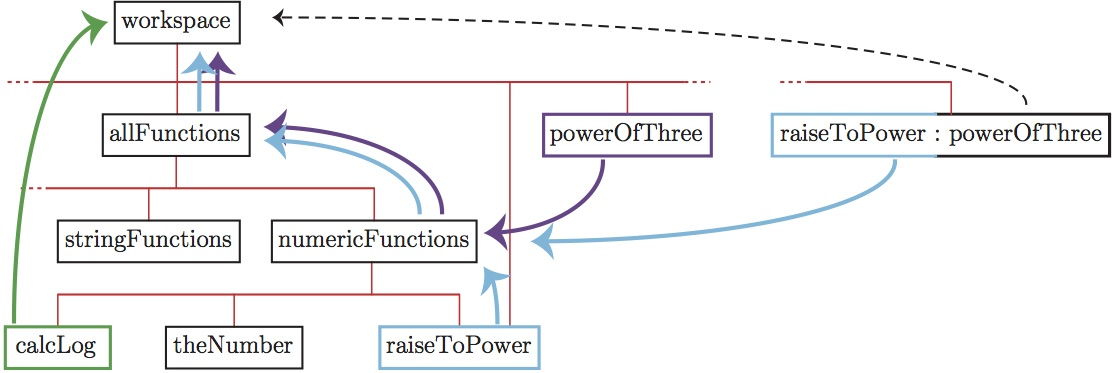
\includegraphics[width=\textwidth]{searchPaths}
\caption{Search paths of various functions from an example in the text.  For simplicity we've named each variable/function box by the member that defined it.  Search paths are shown with heavy arrows:  green arrows for \texttt{calcLog()}; light blue arrows for \texttt{raiseToPower()}; and purple arrows for \texttt{raiseToPower()} function \emph{substituted into} \texttt{powerOfThree()}.  A hypothetical function derived from \texttt{raiseToPower()} and specialized by \texttt{powerOfThree()} (using the inheritance operator) would have each half its code follow its respective original search path (blue and dotted black arrows from the box at right).}
\label{searchPaths}
\end{figure}

The define operator is special in that it always defines the member right in the first variable of the search path.  So \verb#theNumber# will be defined inside \verb#raiseToPower# even if there is another member called \verb#theNumber# further up the search path.

The notion of a search path gives us a more accurate explanation of code substitution:  that operation just changes the \emph{first step} on the search path of the substituted code.  Suppose we write

\begin{code} \begin{verbatim}
(powerOfThree << allFunctions.numericFunctions.raiseToPower)(2)
\end{verbatim} \end{code}

\noindent Then the search path for the substituted function begins at \verb#powerOfThree# but then passes on to \verb#numericFunctions#, \verb#allFunctions#, and the workspace variable just as before.  This is the purple path in Figure \ref{searchPaths}.  Of course the substitution is temporary, but when the substituted function is run it has a permanent effect on \verb#powerOfThree#:  it creates a member inside of it called \verb#theNumber#.  That member will inherit the spliced search path of the substituted code.

\index{search paths|)}\index{functions|)}







% -----------------  Classes & Inheritance  ----------------


\subsection{Classes and Inheritance}\index{classes|(}

A pair of Cicada's curly braces is a versatile object:  it can define not only data types, composite variables, sets and functions but also objects that look somewhat like C++ classes.





% -----------------  Classes  ----------------


\subsubsection{Classes}

A Cicada class, or class instance, is nothing more than a composite variable having both members to variables and members to methods (functions).

\begin{code} \begin{verbatim}
myClassObject :: {
    data :: int
    moreData :: string
    
    init :: {
        code
        { data, moreData } = { 1, "blank" }
    }
    
    otherMethod :: { ... }
}
\end{verbatim} \end{code}

\noindent In a sense, all we have done is point out that functions such as \verb#init()# can be defined inside of composite variables.

To make our class object more C-like we can give it a proper constructor.  All we need to do is take the constructor code from the \verb#init()# method and put it somewhere after the class member definitions.

\begin{code} \begin{verbatim}
myClassObject :: {
    data :: int
    moreData :: string
    
    { data, moreData } = { 1, "blank" }
    
    otherMethod :: { ... }
}
\end{verbatim} \end{code}

\noindent Now both \verb#myClassObject# and each class instance such as \verb#obj1 :: myClassObject# begins initialized to \verb${ 1, "blank" }$.  We can even bundle the constructor code together with the member definitions:

\begin{code} \begin{verbatim}
myClassObject :: {
    data := 1
    moreData := "blank"
    
    otherMethod :: { ... }
}
\end{verbatim} \end{code}

We call these bits of code constructors because they run when the object is created.  C++ constructors also run when an object is created, but they can also be rerun by calling a special function.  How can a Cicada constructor be rerun?  One way is simply to redefine the object:

\begin{code} \begin{verbatim}
myClassObject :: myClassObject
\end{verbatim} \end{code}

\noindent but there is a better way.  Just as in C++, we can also run the constructor as a function.

\begin{code} \begin{verbatim}
myClassObject#0()    | code #0 is the constructor
\end{verbatim} \end{code}

\noindent It turns out that this same trick can also reinitialize members of functions, by rerunning everything up to the \verb#code# marker.  Remember that code number 1, the default function code, begins \emph{after} the first \verb#code# marker or semicolon; therefore the constructor code, which is code number 0, comprises everything \emph{leading up to} that first \verb#code# marker.  In the case of a class object, there is no \verb#code# marker, so the constructor is everything inside of the curly braces.

There is no destructor in Cicada.  In fact there isn't even a direct way to delete an object -- we can only \verb#remove# members leading to an object.  Only when Cicada discovers an object to be completely cut off from the user will dispose of the object and free its memory.  (It's not particularly good at finding these objects though -- to help it out use the \texttt{springCleaning()} function.)\index{classes|)}






% -----------------  Inheritance  ----------------


\subsubsection{Inheritance}\index{inheritance|(}

Cicada also supports a sort of inheritance.  The syntax is different from that in C++:  we use a colon `\verb#:#' to separate the parent object from the code that specializes it.  For example, to derive an object from \verb#myClassObject# we could write:

\begin{code} \begin{verbatim}
myDerivedClassObject :: myClassObject : {
    newString := "hello, I am a new string"
}
\end{verbatim} \end{code}

\noindent \verb#myDerivedClassObject# has all of the members of the original \verb#myClassObject# such as \verb#data# and \verb#otherMethod()# (see previous section), as well as the new string member \verb#newString#.

In this last example, we specialized a predefined parent object with inlined code within braces, using a single inheritance operator.  But one doesn't have to follow this pattern; we can combine class objects and inlined codes in any number and any combination.

\begin{code} \begin{verbatim}
A :: { var1 :: int }
B :: { } : { var2 :: string }
C :: A : B
D :: B : A
E :: { var3 :: int, var4 :: string } : A : { var5 :: char }
F :: C : { remove var1 }
\end{verbatim} \end{code}

\noindent So for example the type of \verb#C# is effectively \verb#{ var1 :: int } : { } : { var2 :: string }#, whereas \verb#D# is \verb#{ } : { var2 :: string } : { var1 :: int }#.  The definition of \verb#F# shows us that it is possible for a derived object to have \emph{fewer} members than its parent object.

Importantly, the order of inheritance affects an object's type.  \verb#C# has a different type than \verb#D#, so \verb#C :: D# or \verb#C = @D# will cause a type-mismatch error.

Cicada allows \emph{existing} objects to be redefined as a different type only if the new type is derived from its original type.  We can always specialize a member's type by adding more inheritance operators \emph{at the end} of the type specification.  All of the following commands will work in order except the last one.

\begin{code} \begin{verbatim}
C :: A : B               | sure -- was already defined this way
C :: A : B               | we already did this, but fine
C :: C                   | fine -- C equals A : B
C :: C : B               | OK -- now C will be A : B : B
C :: A : B : B : {}      | OK
C :: A : B : B : {}      | error!
\end{verbatim} \end{code}

\noindent The last line failed only because any two inlined types are presumed different -- Cicada is not in the business of comparing what's inside those braces to see if they match up.

Although types can be specialized, they can never generalized.  So typing \verb#F :: C# will cause a type-mismatch error.

The same type-matching rules apply to aliases.

\begin{code} \begin{verbatim}
D ::  B : A              | was already defined this way
G :: B : A : { }
D = @G                   | legal
(D =@ *) :: B : A        | legal
G = @D                   | NOT legal!
\end{verbatim} \end{code}

\noindent Aliasing doesn't change a member's type, which explains why we could reassign \verb#D# to a new variable of its original type.

It turns out that the inheritance operator can derive new types for any composite Cicada object:  variables, sets, even functions.  Inheritance of sets is best thought of as a concatenation of these sets.

\begin{code} \begin{verbatim}
a :: {  Alice, Bob  }
b :: {  Charlie, David  }
c :: a : b
\end{verbatim} \end{code}

\noindent So \texttt{c} contains \texttt{Alice}, \texttt{Bob}, \texttt{Charlie}, \texttt{David}, in that order.

Inheritance of \emph{functions} basically tacks new code at the end of the old (parent) function.  Each sub-code keeps its own original search path (the example of Figure \ref{searchPaths} on page \pageref{searchPaths} shows a situation where these may be different).  Function-inheritance makes the most sense when the function does not return a value (i.e. it's a subroutine), because any \verb#return# statement will prevent the new code from running.  The resulting function contains members from both parent functions.

\begin{code} \begin{verbatim}
absval :: {
    sign :: int
    code
    
    sign = 1
    if args[1] < 0  then sign = -1
    args[1] = that*sign
}

sqrt :: {
    code
    return args^0.5
}

modulus_sqrt :: absval : sqrt
\end{verbatim} \end{code}

Here is a better version of this example, where we use the inheritance operator to specialize a function using a composite object that has no coding section (no \verb#code# marker).

\begin{code} \begin{verbatim}
sqrt :: {
    f :: { ; return args[1] }
    code

    return f(args[1])^0.5
}

modulus_sqrt :: sqrt : {
    remove f
    f :: { ; return abs(args[1])  }
}
\end{verbatim} \end{code}

\noindent So the inheritance operator can conjoin different types of objects:  functions, sets, classes, basically any composite object.  To see how this works, think of any non-function as the constructor part of a function (for example, imagine putting a \verb#code# marker at the very end).  Inheritance in Cicada is really a concatenation of code, whether that be constructor code (the commands before the first \verb#code# marker), the first coding block, or any subsequent code blocks.  In Cicada type is code.  Incidentally, this explains why objects can be specialized but not generalized:  we can always do new things to an existing object, but there's no general way to reverse what's already been done to it.
\index{inheritance|)}



\newpage







% --------------- Customizing the Cicada language --------------

\section{Customizing the Cicada language}

The biggest improvement in Cicada over its predecessor (Yazoo script) is the completely rewritten bytecode compiler.  Along with being simpler, and much faster, Cicada's new compiler makes the language \emph{customizable}.  The entire language description is now contained in two arrays in \verb#cicada.c# instead of being baked into the compiler.  By changing those arrays, we change the syntax of Cicada script.



\subsection{\texttt{cicada.c}}\index{cicada.c@\verb#cicada.c#|(textbf}

Inside the file \verb#cicada.c# (or \verb#cicada.cpp#) lives an array called \verb#cicadaLanguage[]# which defines basically every symbol we find inside of a script.  Each array element is a \verb#commandTokenType# structure variable that defines one operator in the Cicada language:

\begin{code} \begin{verbatim}
typedef struct {
    const char *cmdString;
    ccInt precedence;
    const char *rtrnTypeString;
    const char *translation;
} commandTokenType;
\end{verbatim} \end{code}

\noindent The first string, \verb#cmdString#, is the operator symbol or name as written in Cicada.  Then we give the precedence level of the operator (see Table \ref{OoO_table} on page \pageref{OoO_table}).  Next comes a string that explains to the Cicada compiler what type(s) of object this operator `returns' to the surrounding expression.  The final string, \verb#translation#, either encodes the operator directly as bytecode (Cicada's native language), or else `expands' the operator in terms of other Cicada commands.  The first batch of operators have direct bytecode translation, indicated by the fact that their \verb#translation# begins with a \verb#inbytecode# marker (which concatenates to the following string as an unprintable character).  But for the second group of operators, towards the end and lacking a \verb#inbytecode# marker, the \verb#translation# is just a fragment of a script built from the previous operators.

To add a \emph{new operator} into the language, simply add a new entry to the end of the \verb#cicadaLanguage[]# array, in the indicated space, and fill in the four fields.



\paragraph{\texttt{cmdString:}}  The command string defines what sort of object in the script will be recognized as the operator.  For most operators, operators are recognized by some string of letters, symbols, etc. that marks the operator in the script.  (There is really no restriction on this string other than it consist of printable characters.)  For example, looking through the array we find simple operators like \verb#\# (written with two backslashes in the C string) and \verb#exit#.

Many of the operators take left-hand and/or right-hand arguments, as indicated by keywords like \verb#type3arg# to the left and/or right of the operator string.  These keywords are part of the command string -- they are just unprintable characters that get concatenated to the operator strings (because they are only separated by a space).  For example, the full command string of the define operator is

\begin{code} \begin{verbatim}
type2arg "::" type6arg
\end{verbatim} \end{code}

\noindent The define operator requires both a left-hand expression or argument (the member to define) and a right-hand argument, which can be a member name but also a type like \verb#bool#.  The two arguments therefore have a different `type'.  Looking at the comment before the \verb#cicadaLanguage[]# array, we see that a type 2 argument represents a variable or function, and a type 6 argument represents a code-containing expression, as expected.  Having different types allows the compiler to throw type-mismatch errors when expressions don't make sense.

In some cases two different operators will have the same operator string.  For example, compare `\verb#*#' as a multiplication operator versus the void, or `\verb#-#' as either subtraction or negation.  This is \emph{only allowed} if one of the operators expects a left-hand argument and the other doesn't, so that the compiler will immediately know which of the two operators it is looking at when it sees the operator string in a script.  For example, when it stumbles upon a `\verb#-#', that symbol will be interpreted as a subtraction if there is a dangling expression just to the left, and a negation otherwise.

More complex definitions like \verb#while ... do# can involve several operator strings.

\begin{code} \begin{verbatim}
"while" type5arg "do" type1arg
\end{verbatim} \end{code}

\noindent The pattern is always:  operator strings like `\verb#do#' alternating with arguments.  Sometimes, these complex definitions involve a \verb#optionalargs# keyword:  everything before the keyword is required, but everything afterwards is optional.  For example, the \verb#if# command

\begin{code} \begin{verbatim}
"if" type5arg "then" type1arg optionalargs "else" type1arg
\end{verbatim} \end{code}

\noindent \emph{requires} an \verb#if# and a \verb#then#, but the \verb#else# is optional.

There are 10 allowed argument types:  \verb#type0arg# through \verb#type9arg#.  (Cicada only uses 9 of these types).  There are also a few special types.  A \verb#typeXarg# accepts any type of argument, and is used by the \verb#(...)# operator with \emph{no} left-hand argument (i.e. the grouping operator, not a function call) to allow the user to group any sort of expression, even entire commands.  The \verb#commentarg# keyword denotes an block of text to be entirely ignored until the next operator string is encountered (i.e. everything from a comment bar `\verb#|#' to an end-of-line is skipped).  \verb#chararg# and \verb#stringarg# treat the argument as text containing one or several characters respectively.

Finally, there are several special operators that don't have any operator string at all.  If the operator string is simply \verb#int_constant#, then the operator is read when the compiler encounters a number that it deems to be an integer; and the operator whose operator string is \verb#double_constant# corresponds to a floating-point number.  The \verb#variable_name# operator is assumed to apply whenever the compiler encounters a novel word beginning with a letter (which may be followed by underscores and numbers).  In these three cases the number or word should be thought of as an argument, insofar as the bytecode is concerned.

The final class of special operator strings is the adapters, an important element of Cicada scripting that is explained in the next section.  Suffice to say that there is an adapter for each of the 10 argument types, \verb#type0arg_adapter# through \verb#type9arg_adapter#, along with a \verb#noarg_adapter#.



\paragraph{\texttt{precedence:}}  The precedence level determines how operators are bound into expressions.  The high-precedence operators are grouped most tightly to their neighbors, and evaluated before the low-precedence operators.  Thus \verb#A = 2 * B - 2# is grouped:  \verb#A = ( (2*B) - 2)# because of the three gluing operators `\verb#= * -#', multiplication `\verb#*#' has the highest precedence and assignment `\verb#=#' has the lowest precedence.  The precedence level is just an integer, although notice that \verb#cicada.c# predefines a keyword for each precedence level and uses that names instead in the operator definitions.

The \verb#cicadaLanguageAssociativity[]# array in \verb#cicada.c# explains how to group operators of the same precedence level, when there are no parentheses to break the tie.  This can be important.  For example, multiplication and division operators have precedence level 11, and the eleventh entry of the associativity array (i.e. \verb#cicadaLanguageAssociativity[10]#) is \verb#l_to_r# signifying left-to-right grouping.  Therefore the expression \verb#8/2/4# groups as \verb#(8/2)/4# which equals 1, as opposed to \verb#8/(2/4)# which equals 16.  On the other hand, assignment works at precedence level 5, which has \verb#r_to_l# or right-to-left grouping.  Therefore \verb#A = B = C = 2# groups as \verb#A = (B = (C = 2))#, so that 2 copies to \verb#C#, then to \verb#B#, then to \verb#A#.  If the grouping were the other way, then each assignment would rewrite \verb#A#.

The size of the \verb#cicadaLanguageAssociativity[]# array determines the allowed precedence levels.  So by adding an entry the maximum allowable operator precedence level will be 16.  Anything outside the interval [1, \emph{max\_precedence}] will cause an out-of-range compiler error.



\paragraph{\texttt{rtrnTypeString:}}  Many operators `return' a value to the enclosing expression, and which type(s) of value they are allowed to return is encoded in the return-types string.  For example, the addition operator has the return-types string \verb#"456"#, so its return value can be construed as being of type 4, 5 or 6.  The return types correspond to the argument types from the \verb#cmdString# field, so the expression \verb#A = 2+5# is legal (because the assignment operator expects a type-5 right-hand argument) but \verb#2 + 5 = A# is \emph{illegal} (because the left-hand argument of the assignment operator should be type 2).  Notice how each `type' is really an operator \emph{argument type}:  arguments have one type and entire operators have many, which is maybe backwards to the way we usually think.

There is a special \verb#argXtype# return type which is paired with a \verb#typeXarg# argument type.  This is used by the grouping operator \verb#(...)#, causing the type inside the parentheses (its `argument') to be the type returned back to the enclosing expression.  The parentheses only force a grouping, without affecting the type of the enclosed expression.

An entire script must be of type 0 -- Cicada enforces this using adapters (see below).



\paragraph{\texttt{translation:}}  The last field of an operator definition explains how it will be translated into bytecode.  If the bytecode string begins with a \verb#inbytecode# keyword, then the string contains a list of integers which are the bytecode representation of the operator.  For ease of reading, the bytecode translations in \verb#cicada.c# are built from string macros defined in \verb#cicada.h#.  If there is no \verb#inbytecode# keyword, then the string is interpreted as a fragment of Cicada code that will be translated into bytecode using \emph{previously-defined} operators -- so it is best to define these operators last.

The translation strings of bytecode-coded operators have strings of numbers separated by spaces in their translation strings, but also some funny letters:  `\verb#a#', `\verb#j#' and `\verb#p#'.  The `\verb#a#' letter stands for an argument that is to be substituted into the bytecode at the given location, and is followed immediately (no space) by a number from 1 to 9 indicating \emph{which} argument.  (Cicada only supports up to 9 arguments in an operator.)  For example, the assignment operator has a bytecode string

\begin{code} \begin{verbatim}
inbytecode "8 1 a1 a2"
\end{verbatim} \end{code}

\noindent meaning that the operation consists of two integers (8 followed by 1), then the first (left-hand) argument, and last the second (right-hand) argument.  Each of these arguments can themselves be expressions (think \verb#f().a = 5+cos(b)#), in which case the entire expression translated into bytecode is substituted for the argument.  In \verb#cicada.c# the macro \verb#bcArg(x)# produces the ``\verb#ax#" string, so the assignment operator reads

\begin{code} \begin{verbatim}
inbytecode bc_define(equFlags) bcArg(1) bcArg(2)
\end{verbatim} \end{code}

\noindent where \verb#bc_define(equFlags)# produces a define operator with equate flags:  \verb#"8 1"#.

The `\verb#j#' and `\verb#p#' bytecode symbols are used to specify jump offsets (`\verb#j#' -- effectively gotos) and jump positions (`\verb#p#') in the bytecode.  Offsets are the number of code words to jump ahead \emph{from the offset word} (negative offsets jump backwards), and the cicada compiler calculates these as the difference between a jump (\verb#j#) marker and a target position (\verb#p#) marker.  Each of position/jump marker is followed immediately by a number 1-9 indicating which position to define/jump to.  For example, the bytecode string of the \verb#if#-\verb#then#-\verb#else# command which potentially takes 3 arguments is:

\begin{code} \begin{verbatim}
inbytecode "3 j1 a1 a2 1 j2 p1 a3 p2"
\end{verbatim} \end{code}

\noindent In \verb#cicada.c# the position markers are produced using \verb#bcPosition()# macros, and the jump operators have dedicated macros taking the jump offsets as arguments, so this same operator definition reads

\begin{code} \begin{verbatim}
inbytecode bc_jump_if_false(1) bcArg(1) bcArg(2)
                    bc_jump_always(2) bcPosition(1) bcArg(3) bcPosition(2)
\end{verbatim} \end{code}

\noindent In this case the first bytecode command -- bytecode operator 3 which is the jump-if-false command -- jumps to the position of the first position marker, so the compiler calculates this offset by taking the difference in the code position between the \verb#j1# command and \verb#p1# (which is effectively the beginning of argument 3 because \verb#p1# is not a code word) and puts that value in place of the \verb#j1# word.  Likewise, there is an unconditional jump later on to the end (\verb#j2#).  The third argument \verb#a3# may or may not exist because the third argument is in the optional \verb#else# block:  if there is no \verb#else# then \verb#a3# is basically ignored, but the second position marker is still defined.

Many of the adapter operators (explained in the next section) have \verb#anonymousmember# keywords in their bytecode.  These are replaced by unique (and negative) member IDs that are found nowhere else in the script:  the first use of a \verb#anonymousmember# in the bytecode becomes the number -1, the second use represents a -2 in the bytecode, etc.  These are used to construct hidden members that won't bother anyone by conflicting with user-defined members.

Scripted operators -- those without \verb#inbytecode# keywords -- work basically the same as bytecoded operators except that unfortunately the arguments have to be encoded with special keywords (\verb#arg1# through \verb#arg9#) rather than directly in the string.  For example, a \verb#cicadaLibraryFunction()# function is defined at the beginning of \verb#cicada.c# in bytecode, and the \verb#call()# function uses its definition in its script translation:

\begin{code} \begin{verbatim}
"cicadaLibraryFunction#0(" arg1 ")"
\end{verbatim} \end{code}

\noindent So the command \verb#call("myF", 12)# is first translated into \verb$cicadaLibraryFunction#0("myF", 12)$ before being converted into bytecode.

Some operators (usually comments) have no effect on the bytecode whatsoever, and for those we give neither bytecode nor a script translation but instead write \verb#removedexpression# for their translation string.  The \verb#|* ... *|# comment block uses this keyword, as does the line-continuation operator \verb#&# which ignores everything to the end of the line.  Oddly enough the single-line comment \verb#| ...# doesn't use this keyword, and the reason is that it always breaks two separate commands -- so in terms of bytecode it works a lot like a comma or end-of-line. \index{cicada.c@\verb#cicada.c#|)}





% --------------- Cicada bytecode --------------

\subsection{Cicada bytecode}

Occasionally, we might want to extend the Cicada language in a way that can't be scripted, in which case we have to define our new command directly in Cicada's native `bytecode', using \verb#cicada.h# as a dictionary to the command words.  Scripts run much faster from bytecode than they ever could by reading their original text, but it should be emphasized that Cicada's bytecode is \emph{different from} (and much slower than) raw machine code.  One significant difference is that Cicada's bytecode has a recursive structure, composed of expressions and sub-expressions, just like Cicada script itself.  In fact, there is pretty much a one-to-one correspondence between the symbols (operators) we write in Cicada and bytecode commands, except that the bytecode commands are in a different order.

For example, when we type the following command into the command prompt:

\begin{code} \begin{verbatim}
> area = 3.14 * R^2
\end{verbatim} \end{code}

\noindent Cicada's compiler produces bytecode output that looks roughly like:

\begin{code} \begin{verbatim}
equate [ <area> , product_of ( 3.14, raise_to_power ( <R> , 2 ) ) ]
\end{verbatim} \end{code}

\noindent where we've bracketed the arguments of each bytecode operator.  These are just the arguments of each operator in the script, but the compiler has made two changes.  1) Each operator's arguments \emph{follow} the actual operator command:  for example the equate operator is followed by two immediate arguments which correspond to the expressions to the left and right of the equate symbol in the script.  2) The operators are reordered, in ascending precedence when parentheses don't force otherwise.  The equate is done \emph{last}, so it becomes the \emph{outermost} function in the bytecode.  The trick is to think of every operator as a function in bytecode, and write the function command first followed by its arguments.

There's actually a way we can see bytecode from the command prompt:  by using the slightly anachronistic \verb#disassemble()#\index{disassemble@\texttt{disassemble()}} function (dating from before error messages).

\begin{code} \begin{verbatim}
> bytecodeStr := compile("area = 3.14 * R^2")


> disassemble(bytecodeStr)

equ ( sm $area , mul ( 3.14 , pow ( sm $R , 2 ) ) )
\end{verbatim} \end{code}

\noindent Using this tool we find out that there's a `search-for-member' (\verb#sm#) operator before each member identifier.  The member identifier is simply an integer ID number:  positive ID numbers for user-defined members (counting upwards from 1), and negative ID numbers (counting downwards from -1) for so-called hidden members which the compiler adds to the bytecode.  The `disassembly' doesn't show it but there's also a `constant-floating-point' operator just before the 3.14 constant.  The raw bytecode will look something like:

\begin{code} \begin{verbatim}
> bytecd :: [] int

> bytecd[*] =! compile("area = 3.14 * R^2")

> bytecd

{ 8, 1, 10, 309, 29, 55, 1374389535, 1074339512, 31, 10, 310, 54, 2, 0 }
\end{verbatim} \end{code}

\noindent where each bytecode command is now just a number which we can look up in \verb#cicada.h#.  The two complicated numbers are the bytes of 3.14 broken into integers.  The actual output varies based on machine and also on what has been run beforehand (which determines which member ID numbers are assigned).   Every script ends with a null word, telling the interpreter to either fall back to the enclosing function or else exit the program.



\paragraph{Pathnames} \index{pathnames!in bytecode|(}

Cicada pathnames consist of a sequence of steps starting from some variable.  For example the path 

\begin{code} \begin{verbatim}
myVar.array[5].x
\end{verbatim} \end{code}

\noindent takes 3 steps:  to \verb#array#, to the fifth element, and finally to \verb#x#.  In bytecode the final step is the \emph{outermost} operator, so the entire path looks like

\begin{code} \begin{verbatim}
step_to_member( step_to_index( step_to_member( "array", search_member "myVar" ), 5 ), "x" )
\end{verbatim} \end{code}

\noindent (For speed reasons the `step-to-member' operator takes the member-to-step-to as its first argument, which is backwards from the other step operators.)  Notice that step-to-member continues a path, whereas search-member \emph{begins} a path and so takes one fewer arguments.\index{pathnames!in bytecode|)}




\paragraph{Inlined constants}\index{constants!in bytecode|(}

Each of the five types of inlined constants---Booleans, characters, integers, floating-point numbers and strings---has a unique bytecode operator.  The raw data of the constant follows in subsequent bytecode words (integers).  The data for large constants -- floating-point numbers and many strings -- takes up several bytecode words.

String constants in bytecode use the `Pascal' string convention rather than the C format:  the constant-string operator is the first bytecode word, followed by the \emph{character-length} of the string (also 1 bytecode word), followed by the raw string data ($N$/\verb#size(int)# words rounded up).  There is no terminating character.\index{constants!in bytecode|)}



\paragraph{Flow control commands}\index{flow control!in bytecode|(}

The four flow-control commands in Cicada---\verb#if#, \verb#for#, \verb#while# and \verb#do#---are all higher-order commands that the compiler expands into expressions involving `goto's\index{goto, in bytecode|(}.  Cicada sports three `goto's:  an unconditional jump, and jump-if-true and and jump-if-false operators.  Each goto sequence begins with its bytecode command word followed by a jump offset (1 word).  The jump offset is the number of bytecode words to jump ahead \emph{from the jump offset}, which is negative if we want to jump backwards.  The jump must be take us to the \emph{start of a command} -- otherwise \verb#transform()# throws an error.  In the case of the two conditional gotos, there is a final bytecode expression following the jump offset which is the condition on which to jump.

The most complicated flow-control command is the \verb#for# statement, which basically consists of a \verb#while# along with an assignment (to initialize the counter) and a counter-increment command at the end of the loop.  Notice that if we define a variable inside the \verb#for# loop, as in \verb#for (j::int) in <1, 5>#), then Cicada will plunk the whole expression \verb#j::int# into both the initialization and the increment command, which can slow down short loops considerably.\index{flow control!in bytecode|)}\index{goto, in bytecode|)}



% --------------- define flags  --------------


\subsubsection{\texttt{define} flags} \index{define, flags|(textbf}

Member definition (\verb#::#), assignment (\verb#=#), and aliasing (\verb#=@#) are all done by different flavors of the \emph{define operator}.  What makes them different is their `flags':  a set of binary properties such as:  does this operator define new members? does it copy data? etc.  In bytecode, all 8 flags are stored in a single word immediately following the define-operator bytecode word, just before the left- and right-hand arguments to the operator.  This section is devoted to that single flags bytecode word.

To calculate a flags word for a set of flags, we treat each flag as a binary digit and read out the number in decimal.  For example, the define operator has flags 1, 2, 3 and 5 set, so its flags bytecode word is

\begin{align*}
flag &= (1 << 1 = 2) + (1 << 2 = 4) + (1 << 3 = 8) + (1 << 5 = 32)\\
&= 46
\end{align*}

\noindent (\verb#<<# is the bit-shift operator).  Table \ref{defineFlagsTable} on page \pageref{defineFlagsTable} summarizes the flags words for each Cicada operator.  Clearly most of the 256 possible operators are not predefined in \verb#cicada.c#.\\


\paragraph{Flag 0 -- equate:}  copies data from the source variable into the destination variable.  This is used by both the assignment \verb#=# and define-equate \verb#:=# operators, but \emph{not} the aliasing operators.\\


\paragraph{Flag 1 -- update-members:}  causes the destination member to be updated to the type of the source \emph{variable} (not the source member!).  For example, suppose we write:

\begin{code} \begin{verbatim}
a :: *, b := 5
a = @b

c :: a
\end{verbatim} \end{code}

\noindent Member \verb#a# has no type, but the variable it points to is an integer.  Thus the member named `\verb#c#' will be defined as an integer, because the define operator sets the update-member flag.\\


\paragraph{Flag 2 -- add-members:}  creates the looked-for member if it doesn't already exist inside the current-running function.  Set by all define operators, even \verb#:: @# which doesn't assign a type to a new member but will create it.\\


\paragraph{Flag 3 -- new-target:}  does two things.  1) Creates a new destination \emph{variable} if none existed already (i.e. if the destination member was void), but it will not overwrite an existing variable.  2) This flag also updates (specializes) the type of the destination variable, regardless of whether or not it had just created that variable.  The new type is the type of the source \emph{variable} (not member), so it requires that the source member not be void.

The member-define operator (\verb#*::#) sets the update-members flag, but not the new-target flag, so it operates only on members.  On the other hand, the variable-define operator (\verb#@::#) has its new-target flag set but the update-members flag clear, so it will specialize variable but not member types.  It can however create new members since it sets the add-members flag.  Plain old define (\verb#::#) sets all three flags.\\


\paragraph{Flag 4 -- relink-target:}  instructs Cicada to make the destination member an alias of the source variable.  This flag is set by the equate-at and define-equate-at operators.  The destination (left-hand) must be an entire variable, not certain indices of an array (i.e. \verb#a[*].b = @c# is legal but \verb#a[<2, 3>] = @c# is not).

In a sense, relink-target is the third of three pillars of the def-equate flags.  Whereas post-equate copies data, and update-members and new-target copy code, the relink-target flag copies the target reference (which is something like a pointer) of the source member.\\


\paragraph{Flag 5 -- run-constructor:}  \index{constructor!flag in bytecode|(}causes the constructor of the destination variable to be run after it has been created/having its type updated, but before any data has been copied from the source variable.  The constructor is the part of a script before the first \verb#code# marker or semicolon.  If the variable has several concatenated codes, the constructors of each code are run in order from first code to last.  Primitive variables have no code, so they are unaffected by this flag.

The constructor-run is the 2nd-to-last operation performed by the def-equate operator, with the actual equate being the last.  This is why we are able to copy composite variables in one step:

\begin{code} \begin{verbatim}
comp1 :: { ... }
comp2 := comp1
\end{verbatim} \end{code}

\noindent The new variable \verb#comp2# is defined to have the same code as \verb#comp1#, so when its constructor runs it will grow the same set of members that \verb#comp1# has.  Then the final equate should not have any problems, as long as we didn't modify \verb#comp1# after defining it.\index{constructor!flag in bytecode|)}\\


\paragraph{Flag 6 -- hidden-member:} \index{members!hidden|(} sets the `hidden' flag of any newly-defined member.  Hidden members, which are created by bytecode adapters, can only be accessed by name (which is usually unwriteable).  Array-index operators, assignment operations (\verb#=#), comparisons (\verb#==#), and built-in functions like \verb#print()# all skip over hidden members.\index{members!hidden|)}\\


\paragraph{Flag 7 -- unjammable:} makes a member unjammable, i.e. unable to prevent another member from being resized.  Ordinarily, if two members alias overlapping indices of an array, neither one can resize the array since doing so would also affect the other member.  However, if one member is defined as unjammable, then it cannot jam the other member:  the second member \emph{can} be resized and the first member, which now has the wrong number of indices, becomes `unjammed' -- i.e., inoperable.  An unjammed member has to be re-aliased before it can be used again without causing a void-member error.\index{define, flags|)}\\



% --------------- Functions, revisited --------------

\subsubsection{Adapters}\index{adapters|(}

%As a general rule:  two things in Yazoo that look the same, smell the same and should be different, are probably really the same.

There's something missing in our scripts, and the easiest place to see this is in an ordinary function call:

\begin{code} \begin{verbatim}
f(2, pi)
\end{verbatim} \end{code}

\noindent Realizing that commas are just ends-of-lines, we could write this

\begin{code} \begin{verbatim}
f(
    2
    pi
)
\end{verbatim} \end{code}

\noindent which shows that \verb#2# and \verb#pi# are somehow valid commands.  How can this be?

Let's draw an analogy.  Back in the cave man days, there were probably a lot of sentences like

\begin{code} \begin{verbatim}
rock
\end{verbatim} \end{code}

\noindent which in modern English would be written

\begin{code} \begin{verbatim}
[That which I want to draw your attention to] [is] the rock.
\end{verbatim} \end{code}

\noindent In other words, if a sentence only contains an object, the cave man's brain fills it out by adding some stock subject and verb.  Cicada works exactly the same way:  the stock `subjects and verbs' to use in different situations are the so-called adapters defined in \verb#cicada.c#.  Each adapter allows the compiler to convert some bare expression (analogous to the object of a sentence) to another type (perhaps a `sentence' type), at the price of adding a few bytecode words.  This prevents a type-mismatch error from being thrown by incomplete expressions.

For example, when the user enters the command `\verb#2#', the compiler rolls its eyes and reaches for the type-mismatch error button, because it expected a complete command (a type 1 expression) whereas an \verb#int_constant# can only be construed as types 4, 5 or 6 based on its return-types string in the \verb#cicadaLanguage[]# array.  But then Cicada notices an adapter that works on type-5 objects (called \verb#type5arg_adapter# in \verb#cicada.c#), and moreover that adapter's return-types string includes a ``1" which is what we want.  So the adapter adds its code and the error never happens.  Here is the adapter's bytecode:

\begin{code} \begin{verbatim}
inbytecode "8 173 10" anonymousmember "a1"
\end{verbatim} \end{code}

\noindent The expression to adapt is considered the `argument' and goes in place of \verb#a1#.  Looking at \verb#cicada.h# or the reference section, we could figure out that this adapter turns our expression into something looking like

\begin{code} \begin{verbatim}
var1 := 2
\end{verbatim} \end{code}

\noindent except that the define-equate operator has slightly different define flags (173 instead of 47).  Likewise the expression `\verb#pi#' requires a different adapter that looks like

\begin{code} \begin{verbatim}
var2 := @pi
\end{verbatim} \end{code}

\noindent though again with slightly different flags on the aliasing operator.  A third adapter with a define-like operator creates composite objects, and allows statements like \verb#myVar = { 1, false }#.

The \verb#anonymousmember# keyword is a unique member `name', which is inexpressible by any user.  (The reason is that members the user types are translated into positive member ID numbers in bytecode, whereas anonymous members are assigned sequential negative ID numbers.)  Thus the members we represented as \verb#var1# and \verb#var2# in the last paragraph really don't have those names or any other, so they can only be accessed by index using the bracket operators \verb#[...]#.  (Or by `name'/ID number if we are willing to write our own bytecode.)

Incidentally, anonymous members are also used in ordinary function calls, and in this case those members are also `hidden' because their define operators have the hidden-member flag set.  The hidden flag causes these members to be invisible to the array-index operators:  they can only be accessed by `name' (a.k.a. ID number).  The variables behind these members become the \verb#args# variables when functions are run.  If it helps, think of a function call \verb#f(2, pi)# as if the syntax were \verb#f{2, pi}#, having braces denoting the argument variable.

The exotic define operator flags used by function calls are listed in Table \ref{defineFlagsTable} on page \pageref{defineFlagsTable}.  The rarest bird in this collection, abbreviated \verb#def-c**# (`hidden-define-minus-constructor'), lives exclusively in the function call of a \verb#trap()#\index{trap@\texttt{trap()}} function, defining the \verb#args# variable \emph{without running its constructor} so that \verb#trap()# can do this in a controlled way.

The adapters consistently set the unjammable flag of their define/equate-at operators, preventing them from jamming arrays.  For example, if we call \verb#f(myArray[<2, 4>])# we will still be able to resize \verb#myArray# in the future, and the broken link will be refreshed next time that call to \verb#f()# is made because that reruns the argument constructor.  (In sets this can cause a problem, because the set's constructor is not usually rerun after an array resize.  We can get around this by manually aliasing a member to certain array indices.)  Also, the update-members flag is cleared by all of the adapters, so that the anonymous member can be re-assigned to a variable of a different type (for example if between two iterations of the command \verb#f(a)# member `\verb#a#' gets removed and redefined).

One last type of adapter called \verb#noarg_adapter# replaces missing expressions altogether.  These adapters are necessary to allow blank scripts, or expressions like `\verb#,,#' where no command appeared between the commas, since each comma expects a sentence-type argument.  A final no-argument-adapter allows a script to contain a \verb#return# command without a variable.

Notice that the final set of adapters in \verb#cicada.c/cpp# is used to convert a sentences-type expression (type 1) to a script expression (type 0), by adding a null bytecode word at the end.\index{adapters|)}\\


 



\subsection{Custom-compiling within a script}% \index{functions!in bytecode|(}

For a variety of reasons, we might occasionally want to run a script manually without using the \verb#run()# function.  This involves two steps.  The first step is to produce bytecode, easily done using the \verb#compile()# function.  Second, the \verb#transform()# function gives bytecode a perch on a function's internal code registry.  Here is a simple example:

\begin{code} \begin{verbatim}
myBytecode := compile("myMessage := \"Hello, world!\"; print(myMessage)")

newFunction :: transform(myBytecode)

newFunction()
\end{verbatim} \end{code}

\noindent Manual compilation and transformation is necessary when \verb#user.cicada# has not been loaded, for example when running Cicada from the command prompt with a script-file argument.

Another situation where we will want to compile scripts manually is when we want to run a script that uses a \emph{different syntax} from the default Cicada language.  For example, our script might want to process commands typed by the user, that are in a completely different format from the Cicada language.  We don't want to change \verb#cicada.c# because then none of the other scripts like \verb#start.cicada# will work.  Instead we will need to use the \verb#newCompiler()#\index{setCompiler@\texttt{setCompiler()}|(} function to process the user's input differently from our own scripts.  Here is an example, relying on language-constant definitions in \verb#user.cicada#.

\begin{code} \begin{verbatim}
newLanguage :: [] compiledCommandType
newLanguage[*] = {
    { cat("add  ", type1arg, "to", type1arg), 1, "0",
            cat(inbytecode, "8 173 10", anonymousmember, "27 a1 a2 0") },
    { cat("negative", type1arg), 2, "1", cat(inbytecode, "29 54 -1 a1") },
    { int_constant, 0, "1", cat(inbytecode, "54 a1") },
    { double_constant, 0, "1", cat(inbytecode, "55 a1") }
}
newLanguageAssociativity :: [] int
newLanguageAssociativity[*] = { l_to_r, r_to_l }
newCompilerID := setCompiler(newLanguage, newLanguageAssociativity)

myBytecode := compile(input())
doMath :: transform(myBytecode)

doMath()
printl("The answer is:  ", doMath[1])
\end{verbatim} \end{code}

\noindent Notice how the two array arguments to \verb#newCompilerID()# are exactly the same as the two arrays that specify the language in \verb#cicada.c/cpp#.  For consistency, all of the constants used in the C file (such as \verb#int_constant# and \verb#inbytecode#) are also defined in \verb#user.cicada#.  The main difference is that we have to use the \verb#cat()# function to concatenate strings.  Also, make sure to define both arguments as arrays -- \verb#setCompiler()# will not understand anything inside of curly braces.  As always, any script must have an overall type of 0, which in this case means that any valid script is an `\verb#add#' command.

Cicada always opens with a single compiler -- compiler ID 1 -- so to switch back we can just type the command \verb#newCompiler(1)#.  Calling \verb#newCompiler()# with no arguments returns the ID of the current compiler, without changing which compiler is active.

Functions produced by different compilers live in different namespaces, because each compiler which keeps its own running tally of all member names it has encountered (and how many anonymous members have been made).  But the use of separate compilers does \emph{not} prevent collisions of member names between these functions:  if anything switching compilers makes collisions more likely.  (Any new compiler member will assign member IDs starting from 1 and counting upwards, and that ID is the only thing Cicada sees when the function runs.)  To avoid problems, use \verb#transform()#'s ability to customize the search path so that the calling script is hidden from any transformed bytecode that it produces.\index{setCompiler@\texttt{setCompiler()}|)}


\newpage


% --------------- REFERENCE --------------

\section{Reference}



% --------------- Operators --------------

\subsection{Operators and reserved words}  \index{reserved\_words|(} \index{operators!list of|(}

\small

\noindent
\begin{description}
\item{\verb#,# or line break} :  demarcate commands
\item{\verb#( ... )#} :  group terms in an expression
\item{\verb#X#$\sim$} :  ignore output of expression \verb#X#
\item{\verb#|#} :  single-line comment
\item{\verb#|* ... *|#} :  multiple-line comment
\item{\verb#&#} :  continue command on next line\\
\end{description}

\noindent
Numeric operators:
\begin{description}
\item{\verb#x + y#} :  addition
\item{\verb#x - y#} :  subtraction
\item{\verb#x * y#} :  multiplication
\item{\verb#x / y#} :  division
\item{\verb#x ^ y#} :  raise to a power
\item{\verb#i mod j#} :  modulo (integer only)\index{mod@\texttt{mod}}\\
\end{description}

\noindent
Boolean operators:
\begin{description}
\item{\verb#A == B#} :  if equal
\item{\verb#A ==@ B#} :  if same reference
\item{\verb#A /= B#} :  if not equal
\item{\verb#A /=@ B#} :  if different reference
\item{\verb#A >= B#} :  if greater than or equal to
\item{\verb#A > B#} :  if greater than
\item{\verb#A <= B#} :  if less than or equal to
\item{\verb#A < B#} :  if less than
\item{\verb#A and B#} :  if A and B\index{and@\texttt{and}|textbf} (both arguments are always evaluated)
\item{\verb#A or B#} :  if A or B or both\index{or@\texttt{or}|textbf} (both arguments are always evaluated)
\item{\verb#A xor B#} :  if A or B, but not both\index{xor@\texttt{xor}|textbf}
\item{\verb#not A#} :  true only if A is false\index{not@\texttt{not}|textbf}\\
\end{description}

\noindent
Member/array operators:\index{members|(}\index{arrays|(}
\begin{description}
\item{\verb#A.B#} :  step from A into member B
\item{\verb#[ A ]#} :  step into array index A
\item{\verb#[< A, B >]#} :  step into array indices A through B
\item{\verb#[^ N ]#} :  resize array to given size N, step into all indices 1-N
\item{\verb#[+ A ]#} :  insert index
\item{\verb#[+< A, B >]#} :  insert indices
\item{\verb#[*]#  or  \verb#[]#} :  step to all indices; can resize before \verb#=# or \verb#=!#\index{arrays|)}
\item{\verb#remove A#  or  \verb#[- A ]#  or  \verb#[-< A, B >]#} :  remove member, array index A or indices A through B\\\index{remove@\texttt{remove}}
\end{description}\index{members|)}

\noindent
Define/equate operators:
\begin{description}
\item{\verb#A :: B#} :  define A (member with a variable) with the type of the variable that B points to
\item{\verb#A = B#  or  \verb#A <- B#} :  copy data from B to A
\item{\verb#A := B#} :  define A to type B, copy data from B to A
\item{\verb#A =@ B#  or  \verb#A <- @ B#} :  make A an alias of B\index{aliases}
\item{\verb#A :=@ B#} :  define A and make it an alias of B\index{aliases}
\item{\verb#A @:: B#} :  define A to be of type B (variable type only)
\item{\verb#A *:: B#} :  define A to be of type B (member type only)
\item{\verb#A =! B#  or  \verb#A <- ! B#} :  copy data from B to A; even between dissimilar data types\\
\end{description}

\noindent
Predefined variables:
\begin{description}
\item{\verb#this#} :  the function currently executing\index{this@\texttt{this}}
\item{\verb#parent#  or  \verb#\#} :  the next function up the search path\index{this@\texttt{this}}
\item{\verb#that#} :  variable on the left side of an equate\index{that@\texttt{that}}
\item{\verb#args#} :  the argument variable to the function currently executing\index{args@\texttt{args}}
\item{\verb#top#} :  within array brackets, the number of indices\index{args@\texttt{args}}
\item{\verb#nothing#  or  \verb#*#} :  the void\index{nothing@\texttt{nothing}}\\
\end{description}

\noindent
Program flow:
\begin{description}
\item{\verb#if A then ..., else if B then ..., else ...#} :  do if A, B, etc. are true
\item{\verb#while A do ...,#} :  do as long as A is true
\item{\verb#loop ... until A#} :  do until A is true
\item{\verb#for I in < A, B >  ...#} :  do for a defined number of times
\item{\verb#A( ... )#} :  call A as a function with given arguments
\item{\verb#code#} or \verb#;# :  begin a new code block\index{code@\texttt{code} marker}
\item{\verb#return A#  or  \verb#return#} :  exit function with return variable A (if specified)\index{return@\texttt{return}}
\item{\verb#exit#} :  exit Cicada\index{exit@\texttt{exit}}\\
\end{description}

\noindent
Data types:
\begin{description}
\item{\verb#bool#} :  Boolean
\item{\verb#char#} :  character
\item{\verb#int#} :  integer
\item{\verb#double#} :  floating point
\item{\verb#string#} :  string of characters
\item{\verb#'...'#} :  inlined character constant (one character only)
\item{\verb#"..."#} :  inlined string containing given characters
\item{\verb#{ ... }#} :  inlined function, set, class or data type
\item{\verb#A : B#} :  an inherited type specialized by B from parent type A
\item{\verb#A << B#} :  the code/type of B substituted into the variable space of A
\item{\verb$A # B$} :  the Bth code block of variable A\\
\end{description}

\index{reserved\_words|)} \index{operators!list of|)}

\normalsize






% --------------- Bytecode operators --------------

\subsection{Bytecode operators}  \index{bytecode|(}

Each entry in the following list consists of:  a bytecode command word (which is a number), a name in brackets, and then the arguments for that operator separated by commas.  Arguments in plain text take up a defined number of bytecode words.  Unless otherwise indicated, a fixed-width argument is one word long and should be read as a signed integer.  Arguments in italics are themselves bytecode expressions, which can span arbitrary word-lengths.\\



\begin{description}
\item{0  [ null ]} :  marks the end of a code block

\item{1  [ jump ], offset}\index{goto, in bytecode|(} : jumps the program counter to the position of the offset word plus \emph{offset} bytecode words
\item{2  [ jump-if-true ], offset, \emph{condition}} : jumps the program counter to the position of the offset word plus \emph{offset} bytecode words, if the conditional expression evaluates to true
\item{3  [ jump-if-false ], offset, \emph{condition}} : moves the program counter to the position of the offset word plus offset byetcode words, if \emph{condition} is false\index{goto, in bytecode|)}

\item{4  [ code ]} : delineates the boundary between two code blocks
\item{5  [ return ], \emph{return\_variable}} :  exits the function and returns the specified variable
\item{6  [ user function ], \emph{function\_variable}, \emph{args\_variable}} : runs the given user function with the specified arguments, and returns the return variable (if any).
\item{7  [ built-in function ], \emph{function\_ID}, \emph{args\_variable}} : runs the built-in Cicada function with the given ID and arguments, and sends back any return value

\item{8  [ define ], flags, \emph{LH\_var}, \emph{RH\_var}} : applies the define/equate/equate-at command specified by the flags from the source \emph{RH\_var} to the target \emph{LH\_var}
\item{9  [ forced\_equate ], \emph{LH\_var}, \emph{RH\_var}} : copies the raw data from the source \emph{RH\_var} into the target \emph{LH\_var} if their byte-sizes match

\item{10  [ search member ], ID} : searches backwards from the current function for the member having the given ID
\item{11  [ step to member ], ID, \emph{starting\_variable}} : steps to the member with the given ID from the given starting variable
\item{12  [ step to index ], \emph{starting\_variable}, \emph{index}} : steps into the given index of the starting variable
\item{13  [ step to indices ], \emph{starting\_variable}, \emph{low\_index}, \emph{high\_index}} : steps simultaneously into the given range of indices from the starting variable
\item{14  [ step to all indices ], \emph{starting\_variable}} : steps into all indices of the starting variable
\item{15  [ resize ], \emph{variable}, \emph{top\_index}} : resizes the variable's member to have the given number of indices, and steps into these indices
\item{16  [ insert index ], \emph{variable}, \emph{new\_index}} : adds a new index to \emph{variable} at position \emph{new\_index}
\item{17  [ insert indices ], \emph{variable}, \emph{new\_low\_index}, \emph{new\_high\_index}} : adds the new range of indices to \emph{variable} beginning at \emph{low\_index}
\item{18  [ remove ], \emph{member}} : deletes the member or part of the member that was stepped into

\item{19  [ if equal ], \emph{expr1}, \emph{expr2}} : returns true if the two expressions' data are equal; false otherwise
\item{20  [ if not equal ], \emph{expr1}, \emph{expr2}} : returns false if the two expressions' data are equal and true otherwise
\item{21  [ if greater-than ], \emph{num1}, \emph{num2}} : returns true if and only if \emph{num1} is greater than \emph{num2}
\item{22  [ if greater-than-or-equal ], \emph{num1}, \emph{num2}} : returns true if and only if \emph{num1} is greater than or equal to \emph{num2}
\item{23  [ if less-than ], \emph{num1}, \emph{num2}} : returns true if and only if \emph{num1} is less than \emph{num2}
\item{24  [ if less-than-or-equal ], \emph{num1}, \emph{num2}} : returns true if and only if \emph{num1} is less than or equal to \emph{num2}
\item{25  [ if same reference ], \emph{expr1}, \emph{expr2}} : returns true if the two members point to the same data; false otherwise
\item{26  [ if different reference ], \emph{expr1}, \emph{expr2}} : returns false if the two members point to the same data and true otherwise

\item{27  [ add ], \emph{num1}, \emph{num2}} : returns the sum of its numeric arguments
\item{28  [ subtract ], \emph{num1}, \emph{num2}} : returns \emph{num1} minus \emph{num2}
\item{29  [ multiply ], \emph{num1}, \emph{num2}} : returns the product of its numeric arguments
\item{30  [ divide ], \emph{num1}, \emph{num2}} : returns \emph{num1} divided by \emph{num2}
\item{31  [ power ], \emph{num1}, \emph{num2}} : returns \emph{num1} raised to the power \emph{num2}
\item{32  [ modulo ], \emph{num1}, \emph{num2}} : returns the remainder of \emph{num1} divided by \emph{num2} after they have been truncated to integers

\item{33  [ not ], \emph{condition}} : returns true if the condition is false and false if the condition is true
\item{34  [ and ], \emph{condition1}, \emph{condition2}} : returns true if and only if both conditions are true (both are always evaluated)
\item{35  [ or ], \emph{condition1}, \emph{condition2}} : returns true if and only if one or both of the conditions are true (both are always evaluated)
\item{36  [ xor ], \emph{condition1}, \emph{condition2}} : returns true if and only if one, but not both, conditions are true

\item{37  [  code number ], \emph{code number},  \emph{var}} : causes an enclosing function call to execute the given \emph{code number} of \emph{var}
\item{38  [ substitute code ], \emph{code},  \emph{var}} : returns \emph{var} but paired with the given \emph{code} instead of its native code
\item{39  [ append code ],  \emph{f1}, \emph{f2}} : returns \emph{f1} but with the concatenated code \emph{f1} + \emph{f2} instead of its native code

\item{40  [ args ]} : returns the \verb#args# variable for the current function
\item{41  [ this ]} : returns the function variable that is currently running
\item{42  [ that ]} : returns the variable on the left-hand side of the equate statement
\item{43  [ parent ]} : returns the parent of the currently-running function
\item{44  [ top ]} : returns the highest index of the enclosing array brackets
\item{45  [ nothing ]} : returns no variable

\item{46  [ array ],  \emph{num\_indices}, \emph{type}} : an array of \emph{num\_indices} elements of \emph{type}
\item{47  [ bool ]} : Boolean data type\index{bool@\texttt{bool}}
\item{48  [ char ]} : character data type\index{char@\texttt{char}}
\item{49  [ int ]} : integer data type\index{int@\texttt{int}}
\item{50  [ double ]} : floating-point data type\index{double@\texttt{double}}
\item{51  [ string ]} : string data type\index{string@\texttt{string}|textbf}

\item{52  [ constant bool ], num} : returns the Boolean stored in \emph{num} (one bytecode word)
\item{53  [ constant char ], num} : returns the character stored in \emph{num} (one bytecode word)
\item{54  [ constant int ], num} : returns the integer stored in \emph{num} (one bytecode word)
\item{55  [ constant double ], num} : returns the floating-point number stored in \emph{num} (\emph{num} is \verb#sizeof(double)/sizeof(int)# bytecode words long)
\item{56  [ constant string ], characters\_num, string\_data} : returns an inlined string having the given number of characters.  The string\_data field occupies one bytecode word for every four characters.
\item{57  [ code block ]} : returns the inlined code beginning with the next bytecode sentence and ending with a 0 bytecode word


\end{description}
\index{bytecode|)}




% --------------- Def-general operators and flags --------------

\subsubsection{Define operator flags}\index{def-general, flags|(} \index{operators!def-general|(}


Table \ref{defineFlagsTable} lists the common define/equate/equate-at operators and their associated bytecode flag words (the bytecode word following the define operator).  Each flag word encodes the various binary properties of a define operator:  it is the decimal representation of the columns in the table treated as binary digits (where a checkmark equals 1).  The flags are:  equate (0), update-members (1), add-members (2), new-target (3), relink-target (4), run-constructor (5), hidden (6), and unjammable (7).  The last six operators that have asterisks in their names cannot be written into a script, but are generated automatically by the compiler in various situations.\\

\begin{table}
\begin{center}
\begin{tabular}{|c|c|c|c|c|c|c|c|c|c|c|c|}
\hline
{\bf name} & {\bf abbr} & {\bf symbol} & {\bf flags} & {\bf 7} & {\bf 6} & {\bf 5} & {\bf 4} & {\bf 3} & {\bf 2} & {\bf 1} & {\bf 0}\\
\hline \hline
define & def & \verb#::# & 46 & & & \checkmark & & \checkmark & \checkmark & \checkmark &\\
member-define & mdf & \verb#*::# & 6 & & & & & & \checkmark & \checkmark &\\
variable-define & vdf & \verb#@::# & 44 & & & \checkmark & & \checkmark & \checkmark & &\\
\hline
equate & equ & \verb#=# & 1 & & & & & & & & \checkmark \\
define-equate & deq & \verb#:=# & 47 & & & \checkmark & & \checkmark & \checkmark & \checkmark & \checkmark \\
\hline
equate-at & eqa & \verb#=@# & 16 & & & & \checkmark & & & &\\
define-equate-at & dqa & \verb#:=@# & 22 & & & & \checkmark & & \checkmark & \checkmark &\\
\hline
\hline
$\sim$define & def* & N/A & 172& \checkmark & & \checkmark & & \checkmark & \checkmark & &\\
$\sim$define-equate & deq* & N/A & 173 & \checkmark & & \checkmark & & \checkmark & \checkmark & & \checkmark \\
$\sim$define-equate-at & dqa* & N/A & 148 & \checkmark & & & \checkmark & & \checkmark & &\\
\hline
$\sim$define & def** & N/A & 236 & \checkmark & \checkmark & \checkmark & & \checkmark & \checkmark & &\\
$\sim$define-equate & deq** & N/A & 237 & \checkmark & \checkmark & \checkmark & & \checkmark & \checkmark & & \checkmark \\
$\sim$define & def-c** & N/A & 204 & \checkmark & \checkmark & & & \checkmark & \checkmark & &\\
\hline
\end{tabular}
\end{center}
\caption{The flags of all various define, assignment and aliasing operators}
\label{defineFlagsTable}
\end{table}\index{def-general, flags|)} \index{operators!def-general|)}






% --------------- Cicada functions --------------

\subsection{Cicada built-in functions} \index{functions!built-in|(}

Cicada provides a number of built-in functions that work just like user-defined functions.  These are listed in the Table \ref{built_in_IDs}.  A function's ID number is just its `name' in bytecode -- we don't usually have to deal with this.  Functions that leave behind a value when used as a command (i.e. print a value from the command prompt) have checkmarks in the `@' column.  This section explains each built-in function in alphabetical order.

\begin{table}
\begin{center}
\begin{tabular}{|c|c|c||c|c|c||c|c|c|}
\hline
{\bf ID} & {\bf name} & {\bf @} & {\bf ID} & {\bf name} & {\bf @} & {\bf ID} & {\bf name} & {\bf @}\\
\hline \hline
0 & call & & 10 & trap & & 20 & tan & \checkmark\\
\cline{1-3}
1 & setCompiler & \checkmark & 11 & throw & & 21 & acos & \checkmark\\
\cline{4-6}
2 & compile & \checkmark & 12 & top & \checkmark & 22 & asin & \checkmark\\
3 & transform & & 13 & size & \checkmark & 23 & atan & \checkmark\\
\cline{1-3} \cline{4-6}
4 & load & \checkmark & 14 & abs & \checkmark & 24 & random & \checkmark\\
\cline{7-9}
5 & save & & 15 & floor & \checkmark & 25 & find & \checkmark\\
\cline{7-9}
6 & input & \checkmark & 16 & ceil & \checkmark & 26 & type & \checkmark\\
7 & print & & 17 & log & \checkmark & 27 & member\_ID & \checkmark\\
\cline{1-3}
8 & read\_string & & 18 & cos & \checkmark & 28 & bytecode & \checkmark\\
\cline{7-9}
9 & print\_string & & 19 & sin & \checkmark & 29 & springCleaning & \\
\hline
\end{tabular}
\caption{Built-in functions, by bytecode ID number.  Functions which return values even as commands have a checkmark in the `@' columns}\index{types!primitive}
\label{built_in_IDs}
\end{center}
\end{table}




% abs()

\paragraph{\texttt{abs()}\\\\
\normalfont \emph{syntax: } (numeric) \emph{y} = \texttt{abs}((numeric) \emph{x})\\\\}
\index{abs@\texttt{abs()}|(}

Returns the absolute value of its argument (which must be a number).\\

\index{abs@\texttt{abs()}|)}



% acos()

\paragraph{\texttt{acos()}\\\\
\normalfont \emph{syntax: } (numeric) \emph{y} = \texttt{acos}((numeric) \emph{x})\\\\}
\index{acos@\texttt{acos()}|(}

Returns the inverse cosine of its argument.  The argument must be a number on the interval [-1, 1] (a number outside this range will generate the `not a number' value on many machines).  The result is on the interval [0, $\pi$].\\

\index{acos@\texttt{acos()}|)}



% asin()

\paragraph{\texttt{asin()}\\\\
\normalfont \emph{syntax: } (numeric) \emph{y} = \texttt{asin}((numeric) \emph{x})\\\\}
\index{asin@\texttt{asin()}|(}

Returns the inverse sine of its argument.  The argument must be a number on the interval [-1, 1] (a number outside this range will generate the `not a number' value on many platforms).  The result is on the interval [$-\pi/2$, $\pi/2$].\\

\index{asin@\texttt{asin()}|)}




% atan()

\paragraph{\texttt{atan()}\\\\
\normalfont \emph{syntax: } (numeric) \emph{y} = \texttt{atan}((numeric) \emph{x})\\\\}
\index{atan@\texttt{atan()}|(}

Returns the inverse tangent of the argument, which must be numeric.  The result is an angle in radians on the interval [$-\pi/2$, $\pi/2$].\\

\index{atan@\texttt{atan()}|)}





% bytecode()

\paragraph{\texttt{bytecode()}\\\\
\normalfont \emph{syntax: } (string) \emph{codeString} = \texttt{bytecode}((variable) \emph{myFunction} [, (numeric) \emph{memberIndex}])\\\\}
\index{bytecode@\texttt{bytecode()}|(}

Returns the bytecode of a given variable or member.  If there is one argument it returns the bytecode of that variable; if there are two members then it returns the bytecode of member \verb#myFunction[memberIndex]#.  Member code is never run directly, but it determines the sort of variable a member can point to (because \emph{code} and \emph{type} are equivalent in Cicada).

To read the bytecode we need to move the bytecode data from the string into an array of integers using the \verb#=!# operator.  The last integer is always 0, signifying the end of bytecode.  If there are multiple codes (due to the inheritance operator) then the codes are concatenated in parent-to-child order in the same string, and each separate code ends in a null integer.  \texttt{bytecode()} is the inverse operation to \texttt{transform()}.

The \verb#bytecode()# function return the code for functions, but also many other objects that we don't normally think of as having code.  In fact the only restriction is that \verb#myFunction# must be some composite object (defined using curly braces).  So if we define

\begin{code} \begin{verbatim}
pow :: {
    params :: { x :: y :: double  }
    
    code
    
    params = args
    return new(params.x^params.y)
}
\end{verbatim} \end{code}

\noindent then \verb#bytecode(pow)# returns the bytecode for everything inside \verb#pow()#'s definition (including the definition of \verb#params# and the \verb#code# marker), whereas \verb#bytecode(pow.params)# is also legal and returns the bytecode corresponding to \verb#x :: y :: double#.\\

\index{bytecode@\texttt{bytecode()}|)}




% call()

\paragraph{\texttt{call()}\\\\
\normalfont \emph{syntax: } (numeric) \emph{return\_code} = \texttt{call}((string/numeric) \emph{C\_routine}, [\emph{arguments}])\\\\}
\index{call@\texttt{call()}|(textbf}

Runs a user-defined C or C++ routine referenced in \verb#UserFunctions[]# (in \verb#userfn.c# or \verb#userfn.cpp#).  The first argument specifies which function to run, either as a string containing the Cicada function name (the string in \verb#UserFunctions[]#), or else as the array index (beginning at 1) of the function in \verb#UserFunctions[]#.  The subsequent arguments form the \texttt{argv} array that the C routine receives.  Returns the return value of C/C++ function (an integer).

For example, if we write some C function

\begin{code} \begin{verbatim}
ccInt myFunction(ccInt argc, char **argv)  {  ...  }
\end{verbatim} \end{code}

\noindent just as if it were a complete program.  In order to use it from inside Cicada we would add an entry to the \verb#UserFunctions[]# array in \verb#userfn.c#.

\begin{code} \begin{verbatim}
userFunction UserFunctions[] = { { "pass2nums", &pass2nums }, { "cicada", &runCicada },
                { "runFunctionInC", &myFunction } };
\end{verbatim} \end{code}

\noindent \verb#callFunctionInC# is Cicada's name of the function, even though \verb#myFunction# is its C name.  Then, after recompiling Cicada, we could run the function with the command

\begin{code} \begin{verbatim}
result := call("runFunctionInC", arg1, 14, "another argument")
\end{verbatim} \end{code}

\noindent or

\begin{code} \begin{verbatim}
result := call(3, arg1, 14, "another argument")
\end{verbatim} \end{code}

\noindent (because \verb#runFunctionInC# is the 3rd C function in \verb#UserFunctions[]#).  If we are using a string to specify the C function, then we can also use a shorthand syntax where that string follows a dollar-sign:

\begin{code} \begin{verbatim}
result := $runFunctionInC(arg1, 14, "another argument")
\end{verbatim} \end{code}

The number of arguments is passed through \texttt{argc}, and the address of the array of pointers to the actual arguments is located at \texttt{argv}.  So \texttt{argv[0]} is the pointer to the first argument, and \texttt{argv[0][0]} is the first byte of the first argument; \texttt{argv[1][0]} is the pointer to the second argument; etc.

Only primitive variables can compose an argument to the C routine; a composite argument to \texttt{call()} generally contains, and is passed as, multiple primitive arguments, one for each primitive component.  In the example above the number of arguments is at least 3, depending on the type of \verb#arg1#.  Suppose \verb#arg1# was an array of \verb#{ bool, double }# -- then the number of arguments is 4.  (The first argument is an array of \verb#bool#s, the second is an array of \verb#double#s, the third contains the integer 14, and the fourth is a string).  Strings are passed as linked lists (see the reference section).  Void arguments or members are skipped.

\texttt{call()} also adds one final argument at the end, in position \verb#argv[argc]#, that can be used for type-checking.  This argument-info array is a list of elements of type \verb#arg_info#, defined in \verb#userfn.h#:

\begin{code} \begin{verbatim}
typedef struct {
    ccInt argType;
    ccInt argIndices;
} arg_info;
\end{verbatim} \end{code}

\noindent There is one entry in this array for each argument passed by the user.  The \verb#argType# codes are defined in Table \ref{types_table} on page \pageref{types_table}.  \verb#argIndices# gives the number of indices that were passed (1 if it was just a variable, $N$ if an array).

All arguments are passed by reference:  they are pointers to Cicada's own data storage, so data can be exported as well as imported.  It is easy to crash Cicada by overwriting the wrong regions of memory:  a \texttt{call()} preceding a crash is frequently at fault, even if the crash happens far downstream.\\

\index{call@\texttt{call()}|)textbf}




% ceil()

\paragraph{\texttt{ceil()}\\\\
\normalfont \emph{syntax: } (numeric) \emph{y} = \texttt{ceil}((numeric) \emph{x})\\\\}
\index{ceil@\verb$ceil()$|(}

Returns the nearest integer that is as high as or higher than the argument, which must be numeric.  For example, \verb$ceil(5.6)$ returns 6, \verb$ceil(-5.6)$ returns -5, and \verb$ceil(2)$ returns 2.\\

\index{ceil@\verb$ceil()$|)}


 

% compile()

\paragraph{\texttt{compile()}\\\\
\normalfont \emph{syntax: } (string) \emph{script\_bytecode} = \texttt{compile}((string) \emph{script} [, (string) \emph{file\_name} [, (string) \emph{char\_positions} [, member\_names]]])\\\\}
\index{compile@\texttt{compile()}|(textbf}

Before Cicada can execute a script, that script must be compiled into a binary form called bytecode that is much easier to execute than the raw text.  The built-in \texttt{compile()} function does this job.  Given a string containing a Cicada script (\verb#script#), \verb#compile()# then returns a second string (\verb#script_bytecode#) containing Cicada bytecode.  Importantly, the bytecode is \emph{not} machine code -- it is only used by Cicada.

A basic \verb#compile()# call looks like:

\begin{code} \begin{verbatim}
myBytecode := compile("x = 3")
\end{verbatim} \end{code}

\noindent This command produces bytecode using the currently-active compiler.  Each compiler keeps a record of all variable names, so if \verb#x# had been defined with bytecode produced by the current compiler then this command will run just fine.  To change compilers use the \verb#setCompiler()# command.

A compilation error will actually crash the script running the \verb#compile()# command.  To prevent this we can enclose the \verb#compile()# call inside of the \verb#trap()# function.  If we want to print out the error message, we can write a semicolon or \verb#code# marker at the beginning of \verb#trap()#'s arguments.

\begin{code} \begin{verbatim}
> trap(; compile("x = "))

Error:  right-hand argument expected

x =
  ^
\end{verbatim} \end{code}

\noindent The optional second \verb#file_name# argument causes any error message to reference that file name.

\begin{code} \begin{verbatim}
> trap(; compile("x = ", "myFile.txt"))

Error:  right-hand argument expected in file myFile.txt
\end{verbatim} \end{code}

Often a script will compile but cause an error when it runs.  In order to properly flag runtime error messages we must collect another piece of information:  the character position in the original script of each bytecode word.  This lets the error message flag the offending line in the original script.  The character positions are stored inside of any string that is passed as an optional third argument to \texttt{compile()}.  Both that string and the original Cicada script will be passed to \verb#transform()#, the function that actually allows compiled bytecode to be run.

In some cases we may want to avoid using \verb#compile()#, but instead hand-code the bytecode and load it in using \verb#transform()#.  After all, \texttt{compile()} is `only' a string operation:  it converts an ASCII script into a string containing binary bytecode.\\

 \index{compile@\texttt{compile()}|)textbf}
 




% cos()

\paragraph{\texttt{cos()}\\\\
\normalfont \emph{syntax: } (numeric) \emph{y} = \texttt{cos}((numeric) \emph{x})\\\\}
\index{cos@\texttt{cos()}|(}

Returns the cosine of its argument.  The argument must be numeric.\\

\index{cos@\texttt{cos()}|)}
 




% find()

\paragraph{\texttt{find()}\\\\
\normalfont \emph{syntax: } (numeric) \emph{result} = \texttt{find}((strings) \emph{search\_in}, \emph{search\_for} [, (numeric) \emph{mode} [, (numeric) \emph{starting\_position}]])\\\\}
\index{find@\texttt{find()}|(}

Finds an instance of, or counts the number of instances of, a substring (argument 2) within another string (argument 1).  If \texttt{find()} is used in search mode, it returns the character position (where 1 denotes the first character) where the substring was first found, and 0 if it was not found anywhere.  If \texttt{find()} is run in count mode, it returns the number of instances of the substring found within the larger string.

The optional third argument controls the mode that \texttt{find()} is run in:  it needs to be -1, 0 or 1.  If a mode is not specified then it defaults to mode 1, which denotes a forward search; i.e. it will return the first instance of the substring that it finds.  Mode -1 corresponds to a reverse search, which will find the last instance of the substring.  Mode 0 is the count mode.

By default, a forward search begins from the first character, and a reverse search begins with the last character.  A count proceeds forward from the first character.  The starting character can be changed by specifying a starting position in the fourth argument.  A mode has to be given in order for a starting position to be specified.\\

\index{find@\texttt{find()}|)}




% floor()

\paragraph{\texttt{floor()}\\\\
\normalfont \emph{syntax: } (numeric) \emph{y} = \texttt{floor}((numeric) \emph{x})\\\\}
\index{floor@\verb$floor()$|(}

Returns the nearest integer that is as low as or lower than the (numeric) argument.  For example, \verb$floor(2.3)$ returns 2, \verb$floor(-2.3)$ returns -3, and \verb$floor(-4)$ returns -4.\\

\index{floor@\verb$floor()$|)}




% input()

\paragraph{\texttt{input()}\\\\
\normalfont \emph{syntax: } (string) \emph{str} = \texttt{input}()\\\\}
\index{input@\texttt{input()}|(}

Reads in a single line from the C standard input (which is usually the keyboard).  \texttt{input()} causes Cicada's execution to halt until an end-of-line character is read (i.e. the user hits return or enter), at which point execution resumes.  The return string contains all characters before, but not including, the end-of-line.  Reading in a null character causes the error ``I/O error" to be thrown.\\

\index{input@\texttt{input()}|)}




% load()

\paragraph{\texttt{load()}\\\\
\normalfont \emph{syntax: } (string) \emph{file\_string} = \texttt{load}((string) \emph{file\_name})\\\\}
\index{load@\texttt{load()}|(} \index{file I/O!loading|(}

Reads a file into a string.  Both ASCII-encoded and binary files can be read this way.  The file name must include a path if the file is not in the default directory, as in ``\texttt{/Users/bob/Desktop/MyFile.txt}".  If there is an error in opening or reading the file (i.e. if the file was not found or there was a permissions problem), then \texttt{load()} returns ``I/O error", signifying that the error comes from the operating system, not Cicada.  The counterpart to \texttt{load()} is \texttt{save()}.

\texttt{load()} searches only in the default directory.  The user.cicada routine \texttt{Load()} extends the built-in \texttt{load()} by searching all paths specified in the \texttt{filePaths[]} array.  (The \texttt{run()} function in user.cicada also searches all \texttt{filePaths[]}.)\\

\index{load@\texttt{load()}|)} \index{file I/O!loading|)}




% log()

\paragraph{\texttt{log()}\\\\
\normalfont \emph{syntax: } (numeric) \emph{y} = \texttt{log}((numeric) \emph{x})\\\\}
\index{log@\texttt{log()}|(}

Returns the natural logarithm (base $e$) of its argument.  The argument must be numeric.  The logarithm is only defined for arguments greater than zero.\\

\index{log@\texttt{log()}|)}




% member_ID()

\paragraph{\texttt{member\_ID()}\\\\
\normalfont \emph{syntax: } (numeric) \emph{mbr\_ID} = \texttt{member\_ID}((composite variable) \emph{var}, (numeric) \emph{member\_number})\\\\}
\index{member_ID@\texttt{member\_ID()}|(}

Returns the ID number of a given member of a composite variable.  The ID is essentially the bytecode representation of the member's name.  Under normal conditions user-defined names are assigned positive ID numbers, whereas hidden members are given unique negative ID numbers.  The variable enclosing the member is the first argument, and the member number is the second argument.\\

\index{member_ID@\texttt{member\_ID()}|)}




% print()

\paragraph{\texttt{print()}\\\\
\normalfont \emph{syntax: } \texttt{print}((vars) v1, v2, ...)\\\\}
\index{print@\texttt{print()}|(} \index{printing!to screen|(}

Writes data to the standard output (which is normally the command prompt window).  The arguments are printed sequentially and without spaces in between.  Numeric arguments are converted to ASCII and printed as legible integers or floating-point numbers.  String arguments are written verbatim (byte-for-byte) to the screen, except that unprintable characters are replaced by their hexadecimal equivalents ``\verb$\AA$" (which is also the format in which these characters may be written into a string).  Also, carriage returns in strings are written as end-of-line characters, so a PC-style line ending marked by ``\verb$\0D\n$" outputs as a double line-break.

When Cicada is run from the command prompt, \verb#user.cicada# loads three further printing functions:  \verb#printl()# (print with line break), \verb#sprint()# (for printing composite structures), and \verb#mprint()# (printing arrays).  \verb#sprint()# is the default function for printing expressions typed by the user.\\

\index{print@\texttt{print()}|)} \index{printing!to screen|)}





% print_string()

\paragraph{\texttt{print\_string()}\\\\
\normalfont \emph{syntax: } \texttt{print\_string}([(numeric) precision,] (string) to\_write, (vars) v1, v2, ...)\\\\}
\index{print_string@\verb$print_string()$|(} \index{strings!type conversion|(} \index{printing!to a string|(}

Writes data to a text string.  \texttt{print\_string()} is the counterpart to \texttt{read\_string()}.  Roughly speaking, \texttt{print\_string()} is to \texttt{print()} as C's more elaborate \texttt{sprintf()} is to \texttt{printf()}.  The string to write is followed by any number of variables whose data Cicada writes to the string (with no spaces in between).  Strings from the source variables get copied into the destination string verbatim.  Numeric variables are written as text, and here \texttt{print\_string} differs from a forced equate.  For example: 

\begin{code} \begin{verbatim}
print_string(str, 5, 2.7)
\end{verbatim} \end{code}

\noindent sets \texttt{str} to ``52.7", whereas

\begin{code} \begin{verbatim}
str =! { 5, 2.7 }
\end{verbatim} \end{code}

\noindent gives something illegible (the raw bytes encoding the two numbers in binary format).

If the first argument is numeric, then it is taken as the output precision for floating-point \texttt{single} and \texttt{double} variables; then the output string must follow as the second argument.  Otherwise the output precision is determined by the C constant \texttt{DBL\_DIG} for \texttt{double}-typed variables.  Thus, when no precision is specified, \texttt{print\_string} prints considerably more digits than does \texttt{print()}.\\

\index{print_string@\verb$print_string()$|)} \index{strings!type conversion|)} \index{printing!to a string|)}




% random()

\paragraph{\texttt{random()}\\\\
\normalfont \emph{syntax: } (numeric) \emph{y} = \texttt{random}()\\\\}
\index{random@\verb$random()$|(}

Returns a pseudo-random number uniformly drawn on the interval [0, 1].  To obtain the random number to double-precision, Cicada calls C's \verb$rand()$ function twice:

\begin{align*}
\texttt{random()} = \texttt{rand()}/\texttt{RAND\_MAX} + \texttt{rand()}/(\texttt{RAND\_MAX})^2\\
\end{align*}

\noindent The random number generator is initialized by Cicada to the current clock time each time the program is run, so the generated sequence should not be repeatable.\\

\index{random@\verb$random()$|)}




% read_string()

\paragraph{\texttt{read\_string()}\\\\
\normalfont \emph{syntax: } \texttt{read\_string}((string) to\_write, (vars) v1, v2, ...)\\\\}
\index{read_string@\verb$read_string()$|(} \index{strings!type conversion|(}

Reads data from an ASCII string into variables.  The first argument is the string to read from; following arguments give the variables that will store the data.  \texttt{read\_string()} is the humble cousin to C's \texttt{sscanf()} routine (it does not take a format string).  The various fields within the string must be separated by white space or end-of-line characters.

\texttt{read\_string()} converts ASCII data in the source string into the binary format of Cicada's memory.  Thus numeric fields in the source string need to be written out as text, as in ``3.14".  Each string field must be one written word long, so ``the quick brown" will be read into three string variables, not one.  Composite variables are decomposed into their primitive components, which are read sequentially from the source string.  Void members are skipped.

Here is an example of the use of \texttt{read\_string()}

\begin{code} \begin{verbatim}
date :: { month :: string, day :: year :: int }
activity :: string
read_string("Jan 5 2007   meeting", date, activity)
\end{verbatim} \end{code}

If the string cannot be read into the given variables (i.e. there are too many or too few variables to read), then \verb#read_string()# throws a type-mismatch warning.  Warnings can also be thrown if \verb#read_string()# cannot read a field that should be numeric, or if there is an overflow in a numeric field.

\texttt{read\_string()} is a counterpart to \texttt{print\_string()}.  However, \texttt{print\_string()} does not write spaces in between the fields, so unless spaces are put in explicitly its output cannot be read directly by \texttt{read\_string()}.\\

\index{read_string@\verb$read_string()$|)} \index{strings!type conversion|)}





% save()

\paragraph{\texttt{save()}\\\\
\normalfont \emph{syntax: } \texttt{save}((strings) \emph{file\_name}, \emph{data\_to\_write})\\\\}
\index{save@\texttt{save()}|(} \index{file I/O!saving|(}

Saves the data from the second argument into the file specified in the first argument.  There is no return value, although the error ``I/O error" will be thrown if the save is unsuccessful.  (An error would likely indicate a bad pathname, disk full, or that we don't have write permissions for that file or directory).  If the directory is not explicitly written before the file name, as in ``\texttt{/Library/my\_file}", then the file is saved in the default directory, which is probably the Cicada directory.

There is no need for the data to be encoded in ASCII format, even though it gets passed to \verb#save()# as a string.  Online conversion to the proper string type can be done in the following way:

\begin{code} \begin{verbatim}
save("my_data", (temp_str :: string) =! the_data)
\end{verbatim} \end{code}

\noindent where \texttt{the\_data} may be a variable or array or any other object.  \texttt{save()} writes the data verbatim; if the data is ASCII text, then a text file will be produced; otherwise the output should be considered a binary file.  The saved data can be read back into a string using the \texttt{load()} function.\\

\index{save@\texttt{save()}|)} \index{file I/O!saving|)}




% setCompiler()

\paragraph{\texttt{setCompiler()}\\\\
\normalfont \emph{syntax: } (numeric) \emph{compilerID} = \texttt{setCompiler}([(numeric) \emph{compilerIDtoUse}])\\\\
\normalfont \emph{or: } (numeric) \emph{compilerID} = \texttt{setCompiler}(array of \{ (string) commandString, (int) precedence, (string) rtrnTypes, (string) translation \}, (int array) opLevelDirections[])\\\\}
\index{setCompiler@\texttt{setCompiler()}|(}

Optionally sets the active compiler, and returns the ID number of the active compiler.  To use a particular compiler, pass its ID number as the first argument.  To simply find the ID number of the current compiler, we can just call \verb#setCompiler()# with no arguments.  To create a new compiler we pass \verb#setCompiler()# having two arguments:  1) an array of \verb#{ string, int, string, string }#, one element for each command, containing the definitions of each command, and 2) an array of the direction to evaluate each order-of-operations level.  These mirror the \verb#cicadaLanguage[]# and \verb#cicadaLanguageAssociativity[]# arrays, respectively, which are defined in \verb#cicada.c#.\\

\index{setCompiler@\texttt{setCompiler()}|)}




% sin()

\paragraph{\texttt{sin()}\\\\
\normalfont \emph{syntax: } (numeric) \emph{y} = \texttt{sin}((numeric) \emph{x})\\\\}
\index{sin@\texttt{sin()}|(}

Returns the sine of its argument, which must be numeric.\\

\index{sin@\texttt{sin()}|)}





% size()

\paragraph{\texttt{size()}\\\\
\normalfont \emph{syntax: } (numeric) \emph{var\_size} = \texttt{size}((var) \emph{my\_var} [, (bool) \emph{physicalSize}])\\\\}
\index{size@\texttt{size()}|(}

Returns the size, in bytes, of the first argument.  For composite variables, this is the sum of the sizes of all its members.  If two members of a composite variable point to the same data (i.e. one is an alias of the other), then that data will indeed be double-counted \emph{unless} the optional second argument is set to \verb#true# (its default value is \verb#false#).  If the second argument if \verb#false# then \verb#size()# returns the number of bytes that will participate in, for example, a forced-equate or \verb#save()#, which may be more than the number of bytes of actual storage which is returned by setting the second argument to \verb#true#.

If a member points back to the composite variable, as in

\begin{code} \begin{verbatim}
a :: {
    self := @this
    data :: int    }

size(a)   | will cause an error
\end{verbatim} \end{code}

\noindent then the size of \texttt{a}, including its members and its members' members, etc., is effectively infinite, and Cicada throws a self-reference error unless the second argument was set to \verb#true#.\\

\index{size@\texttt{size()}|)}





% springCleaning()

\paragraph{\texttt{springCleaning()}\\\\
\normalfont \emph{syntax: } \texttt{springCleaning}()\\\\}
\index{springCleaning@\texttt{springCleaning()}|(}

This function removes all unused objects from Cicada's memory, in order to free up memory.  An object is termed `unused' if it cannot be accessed by the user in any way.  For example, if we \verb#remove# the only member to a function then that function's internal data can never be accessed unless it is currently running.

Cicada tries to free memory automatically, but unfortunately it is not always able to do so.  (The reason is self-referencing loops between objects in memory.)  The only way to eliminate these zombies is to comb the whole memory tree, which is what \texttt{springCleaning()} does.  When Cicada is run from the command prompt, it disinfects itself with a \texttt{springCleaning()} after every command from the user.  But we might want to scrub the memory more often if we are running a lengthy, memory-intensive script that allocates and removes memory frequently.  \verb#springCleaning()# can help unjam arrays, if there is no member leading to the jamb.\\

\index{springCleaning@\texttt{springCleaning()}|)}





% tan()

\paragraph{\texttt{tan()}\\\\
\normalfont \emph{syntax: } (numeric) \emph{y} = \texttt{tan}((numeric) \emph{x})\\\\}
\index{tan@\texttt{tan()}|(}

Returns the tangent of its (numeric) argument.\\

\index{tan@\texttt{tan()}|)}




% throw()

\paragraph{\texttt{throw()}\\\\
\normalfont \emph{syntax: } \texttt{throw}((numeric) error\_code [, (composite) error\_script [, (numeric) concat\_number [, error\_index [, (Boolean) if\_warning]]]])\\\\}
\index{throw@\texttt{throw()}|(}

Causes an error to occur.  This of course stops execution and throws Cicada back to the last enclosing \texttt{trap()} function; if there is none then Cicada either prints an error (if run from the command line) or bails out completely.  The first argument is the error code to throw -- these are listed in Table \ref{errCodeTable} on page \pageref{errCodeTable}.  The optional second, third and fourth arguments allow one to specify the function, the part of the function (should be 1 unless the inheritance operator was used) and the bytecode word in that function the error appears to come from.  If one sets the optional fifth argument to true, then the error will be thrown as a warning instead.  All arguments may be skipped with a `\verb#*#'.

Although all real errors have error codes in the range 1-50, \texttt{throw()} works perfectly well for larger (or smaller) error codes that Cicada has never heard of.  It can be hard to tell when \texttt{throw()} is working.  For starters, if the error code is zero then it will appear that \texttt{throw()} is not doing its job, just because 0 is code for `no error'.  \texttt{throw()} does require that the error code be zero or positive, so it gives a number-out-of-range error if the argument is negative.  However, the following also gives a range error:

\begin{code} \begin{verbatim}
throw(2)
\end{verbatim} \end{code}

\noindent In this case \texttt{throw()} actually worked:  we got an out-of-range error because that is error \#2.  (That once caused the author some confusion..)\\

\index{throw@\texttt{throw()}|)}





% top()

\paragraph{\texttt{top()}\\\\
\normalfont \emph{syntax: } (numeric) \emph{vartop} = \texttt{top}((composite variable) \emph{my\_var})\\\\}
\index{top@\texttt{top()}|(}

Returns the number of indices of the argument variable.  The argument must be a composite variable or equivalent (e.g. set, function, class, etc.).  \texttt{top()} does \emph{not} count hidden members.  Therefore the value it returns corresponds to the highest index of the variable that can be accessed, so

\begin{code} \begin{verbatim}
my_var[top(my_var)]
\end{verbatim} \end{code}

\noindent is legal (unless the top member is void) whereas

\begin{code} \begin{verbatim}
my_var[top(my_var) + 1]
\end{verbatim} \end{code}

\noindent is always illegal (unless we are in the process of defining it).  Notice that in both of these cases we can replace the \verb#top()# function by the \verb#top# \emph{keyword}, which is always defined inside of array brackets:  e.g. \verb#my_var[top+1]#.\\

\index{top@\texttt{top()}|)}




% transform()

\paragraph{\texttt{transform()}\\\\
\normalfont \emph{syntax: } (composite) \emph{target\_function} = \texttt{transform}((string) \emph{bytecode} [, (composite) \emph{target\_function} [, (composite) \emph{code\_path} [, (string) \emph{file\_name} [, (string) \emph{script} [, (string) \emph{char\_positions}]]]]])\\\\}
\index{transform@\texttt{transform()}|(textbf} \index{registers!composite|(} \index{R_composite@\verb#R_composite#|(}

Copies compiled bytecode stored as a string (1st argument) into the internal code of a target function variable (return value and/or 2nd argument), \emph{without} running the code's constructor.  The bytecode is typically generated using the \verb#compile()# function:

\begin{code} \begin{verbatim}
newFunction :: transform(compile("toAdd := 2; return args[1]+toAdd"))
\end{verbatim} \end{code}

\noindent but it is also possible to write the bytecode by hand.  This probably won't work -- the member IDs depend on your workspace history -- but the code looks something like:

\begin{code} \begin{verbatim}
newFunction :: {}
(newBytecode :: string) =! { 8, 47, 10, 314, 54, 2, 4, &
                      5, 8, 237, 10, -999, 27, 12, 40, 54, 1, 10, 314, 0 }
transform(newBytecode, newFunction)
\end{verbatim} \end{code}

\noindent At this point it is as if we had written

\begin{code} \begin{verbatim}
newFunction :: { toAdd := 2; return args[1]+toAdd }
\end{verbatim} \end{code}

\noindent We can now execute the new code by running the target function.

\begin{code} \begin{verbatim}
newFunction(3)        | will return 5
\end{verbatim} \end{code}

When we define a function as the return value of \verb#transform()#, as in the previous example, the constructor runs automatically.  If we don't want this to happen, we should pass in a target function as the second argument of \verb#transform()#.  If a function appears here, that is not void, then that function's existing codes are erased and replaced by the transformed code (assuming no error) without running the constructor.

The default search path for the transformed code is the same search path used the function that called \verb#transform()#, but we can replace this default with a manually-constructed path by passing a set of variables as the optional 3rd argument.  For example

\begin{code} \begin{verbatim}
A :: B :: C :: { D :: {} }
transform(newBytecode, newFunction, { A, C.D, B })
\end{verbatim} \end{code}

\noindent causes \verb#newFunction()#'s search path to go from \verb#newFunction# to \verb#A# to \verb#C.D# and finally end at \verb#B#.

The optional fourth, fifth and sixth arguments help Cicada to give helpful error messages if the new code crashes when we try to run it.  The fourth argument is just the name of the file containing the script, if applicable (otherwise set it to the void).  The fifth argument is the original ASCII text of the script, and the sixth is the mapping between bytecode words and script characters that is an optional output of \verb#compile()#.  Here is how we pass all of this information between \verb#compile()# and \verb#transform()#:

\begin{code} \begin{verbatim}
fileName := "scriptFile.cicada"
myScript := load(fileName)
opPositions :: string

scriptBytecode := compile(myScript, fileName, opPositions)

newFunction :: {}
transform(scriptBytecode, newFunction, { }, fileName, myScript, opPositions)
\end{verbatim} \end{code}

It is certainly possible to pass bogus bytecode to \verb#transform()# (particularly if we're trying to write out the binary ourselves).  \verb#transform()# checks the bytecode's syntax, and if there is a problem then it crashes out with an error message.\\

\index{transform@\texttt{transform()}|)textbf} \index{registers!composite|)} \index{R_composite@\verb#R_composite#|)}




% trap()

\paragraph{\texttt{trap()}\\\\
\normalfont \emph{syntax: } (numeric) \emph{error\_code} = \texttt{trap}([code to run])\\\\}
\index{trap@\texttt{trap()}|(textbf} \index{registers!error and warning|(}

Runs the code inside the parentheses (i.e. its argument), and returns any error value.  Error codes are listed in Table \ref{errCodeTable} on page \pageref{errCodeTable}.  No \texttt{code} marker is needed within a \texttt{trap()} call.  Upon error, the argument stops running and the error code is returned; if the argument finishes with no error then the return value is 0.  \verb#trap()# thus prevents a piece of dubious code from crashing a larger script.  Note that the most egregious errors are compile-time errors and \verb#trap()# will not be able to prevent those -- this includes some type-mismatch errors like \verb#trap(string = 4)#.

A \verb#trap()# call can optionally print out an error message if needed.  To do this we add a semicolon (or \verb#code# marker) immediately at the beginning of its arguments.  A second opening semicolon causes it to print any error message \emph{without} clearing the error -- so code execution will then fall back to the next enclosing \verb#trap()# and possibly print another message.  This can help to trace errors through multiple nested functions.

\begin{code} \begin{verbatim}
trap((a::*) = 2)                   | prevents a crash
errCode := trap((a::*) = 2)        | returns the type-mismatch error code
trap( ; (a::*) = 2)                | prints a type-mismatch error but doesn't cause crash
trap( ; ; (a::*) = 2)              | prints a type-mismatch error, then crashes out
\end{verbatim} \end{code}

\noindent Notice that \verb#trap()# will also print warning messages (minor errors that don't stop the program).  Warning codes are the same as error codes except that they are negated:  for example an out-of-range error will return error code 2, but an out of range warning will return -2.  If several warnings have been produced, \verb#trap()# will only print and return the error code for the last one.

The \verb#trap()# function has the unique ability to run its arguments in whatever function called \verb#trap()#, rather than in a private argument variable used by all other built-in and user-defined functions.  So variables which are defined within the \verb#trap()# argument list will be accessible to the rest of the function.  Also \verb#this# and \verb#parent# have the same meaning inside a \verb#trap()# command as outside of it.

\index{trap@\texttt{trap()}|)textbf} \index{registers!error and warning|)}





% type()

\paragraph{\texttt{type()}\\\\
\normalfont \emph{syntax: } (numeric) \emph{theType} = \texttt{type}((composite variable) \emph{var} [, (numeric) \emph{memberNumber}])\\\\}
\index{type@\texttt{type()}|(}

Returns a number representing the type of the given variable (one argument) or one of its members (if there is a second argument).  The variable is the first argument, and the member number is the second argument.  The types IDs are listed in Table \ref{types_table} on page \pageref{types_table}.  A composite-typed variable or member only returns a `5' even though its full type is properly determined by its code list -- use the \verb#bytecode()# function to obtain the code list.\\

\index{type@\texttt{type()}|)} \index{functions!built-in|)}





% --------------- start.cicada & user.cicada --------------


\subsection{Functions define in Cicada scripts} \index{functions!pre-scripted|(} \index{start.cicada@\texttt{start.cicada}|(}

When Cicada is run from the command line with argument, as in

\begin{code} \begin{verbatim}
user-prompt%./cicada myfile
\end{verbatim} \end{code}

\noindent it runs the user's script \verb#myfile.cicada#.  On the other hand, when Cicada is run without a script file:

\begin{code} \begin{verbatim}
user-prompt% ./cicada
\end{verbatim} \end{code}

\noindent then Cicada runs its own script \verb#start.cicada# which brings up the interactive command prompt.  The first thing \verb#start.cicada# does is to run a second script file \verb#user.cicada# which predefines a number of variables and functions for the user.  Here we list a few relevant contents of the prepackaged start.cicada file, along with the definitions in \verb#user.cicada#.




\subsubsection{\texttt{start.cicada}}

The \verb#start.cicada# script provides an interactive command prompt, while keeping most of its internal functions hidden from the user.  However, a few of its variables and functions have aliases inside the user's workspace, and those are the focus of this section.\\


\paragraph{\texttt{calculator}:}\index{calculator@\texttt{calculator}|(} is a function that prints the results of incomplete expressions at the command line.  An incomplete expression is one that is not assigned to a variable, or used in any other way.  For example, if the user types

\begin{code} \begin{verbatim}
a = 5 + 2
\end{verbatim} \end{code}

\noindent then nothing will be printed, regardless of whether \texttt{calculator} is on or off.  However, if the user were to enter just

\begin{code} \begin{verbatim}
5 + 2
\end{verbatim} \end{code}

\noindent then the answer `7' will be printed, thanks to the calculator.

To be completely technical, the calculator prints the data of all hidden members created by the user.  Since these members will never be used again \verb#start.cicada# removes them after each command from the user, but only after asking the calculator to print them first.  The calculator is only a printing function, not a calculator per-se.

By default, the calculator is aliased to \verb#user.cicada#'s \verb#sprint()# function.  We can change the output style by aliasing it to another printing function:

\begin{code} \begin{verbatim}
> calculator = @mprint
\end{verbatim} \end{code}

\noindent Or, if calculator is getting annoying (e.g. printing the output of functions we don't care about, or that return enormous blocks of data), we can turn it off altogether:

\begin{code} \begin{verbatim}
> calculator = @nothing
\end{verbatim} \end{code}

\index{calculator@\texttt{calculator}|)}



\paragraph{\texttt{ans}:}\index{ans@\texttt{ans()}|(}:  short for ``answer".  This is aliased to whatever the calculator last printed (void if the calculator hasn't printed anything yet).  Use \verb#ans# like any other variable:

\begin{code} \begin{verbatim}
> 2+5

7

> ans*2

14
\end{verbatim} \end{code}

\index{ans@\texttt{ans()}|)}



\paragraph{\texttt{allNames}:}\index{allNames@\texttt{allNames}|(}  the list of member names that have been defined so far, including those defined in \verb#start.cicada#.  \verb#allNames# is updated with every new command-line prompt, or every time the user calls \verb#compile()# with \verb#allNames# as the fourth argument.  This list is used by \verb#user.cidada#'s \verb#go()# and \verb#what()# functions.\index{allNames@\texttt{allNames}|)}


\paragraph{\texttt{go\_path[]}:}\index{go\_path@\texttt{go\_path}}  a set of aliases to each composite object in the search path, beginning with \verb#root# and ending with the current working variable.  \verb#start.cicada# uses \verb#go_path# to form the search path for each command entered by the user.  Both \verb#go()# and \verb#jump()# work by modifying \verb#go_path#, and \verb#start.cicada# will reset \verb#go_path# if it detects a problem.  The user can add a small coding section to \verb#go_path# which \verb#start.cicada# will run if it needs to reset the path; in this coding section do not define any variables or run any functions or problems will start happening.\\\\

\index{start.cicada@\texttt{start.cicada}|)}





\subsubsection{\texttt{user.cicada}} \index{user.cicada@\texttt{user.cicada}|(}

When Cicada is run interactively, \verb#start.cicada# runs the script file \verb#user.cicada# file which simply predefines a number of useful constants and functions in the workspace.  As its name suggests, the user is absolutely encouraged to customize \verb#user.cicada# in whatever way makes it most useful.




\paragraph{Constants and variables}


\paragraph{\texttt{passed}:}\index{passed@\texttt{passed}}  0, denoting the error code of a function that did not cause any error.

\paragraph{\texttt{e}:}\index{e@\texttt{e}}  the exponential constant.  Rather than provide an \texttt{exp()} function, Cicada defines \texttt{e} so that the user can evaluate exponentials by writing \verb#e^x#,  \verb#e^-2#, etc.

\paragraph{\texttt{pi}:}\index{pi@\texttt{pi}}  the famous constant pi.

\paragraph{\texttt{inf}:}\index{inf@\texttt{inf}}  infinity.

\paragraph{\texttt{nan}:}\index{nan@\texttt{nan}}  not-a-number (used by floating-point arithmetic).

\paragraph{\texttt{root}:}\index{root@\texttt{root}}  an alias to the user's workspace.

\paragraph{\texttt{where}:}\index{where@\texttt{where}}  the current search path of the user, stored as a string.

\paragraph{\texttt{filePaths[]}:}\index{filePaths@\texttt{filePaths}|(}  a string array of pathnames to folders.  The \verb#user.cicada# routines (but \emph{not} the built-in Cicada functions!) will search each of these paths when looking for a file.  \verb#user.cicada# preloads the empty path, which is usually the Cicada directory.  We can change the search paths just by manipulating this set:  e.g. \verb#filePaths[+2] = "/Desktop/"#.\index{filePaths@\texttt{filePaths}|)}\\\\\\\\


We will skip the custom compiler definition here since they are explained in Chapter 4.  Next is a function that fixes one of the more awkward aspects of Cicada's use of functions.\\




\paragraph{Function calling}


\paragraph{\texttt{new()}\\\\
\normalfont \emph{syntax: } (same type) \emph{var2} = @\texttt{new}((any type) \emph{var1} [, (variable) \emph{data\_to\_copy}] [ ; modifying code])\\\\}\index{new@\texttt{new()}|(}

The \texttt{new()} function returns a new instance of a variable, of the same type as the old and storing the same data.  This is particularly useful within functions, where, as emphasized earlier, it is usually wise to create a new return variable with each function call.  Instead of writing

\begin{code} \begin{verbatim}
f1 :: {
    ...
    ((rtrn =@ *) @:: double) = x + y
    return rtrn     }
\end{verbatim} \end{code}

\noindent we accomplish this with

\begin{code} \begin{verbatim}
f1 :: {
    ...
    return new(x + y)     }
\end{verbatim} \end{code}

\texttt{new()} will not work if the variable's type does not match its current contents, which can happen if the variable had been modified after being created:

\begin{code} \begin{verbatim}
comp1 :: {  a :: int  }
comp1.b :: char

new(comp1)     | cannot copy the data
\end{verbatim} \end{code}

\noindent In this case \texttt{new()} will create a new variable using \texttt{comp1}'s constructor, but it will not be able to copy the data over and will output a warning.  There are two ways to fix this.  1) The optional second argument to \verb#new()# decouples the variable that provides the type specification (first argument) from the variable that provides the data (second argument).  If this second argument is void (as in \verb#new(v, *)#) then no data is copied.  2) Any coding section in the arguments are run \emph{inside} the new variable immediately after it is created, allowing us to modify the variable before the data is copied.

Note that \verb#new({a, b})# doesn't make new instances of  \verb#a# and \verb#b#, but rather just returns a new set of aliases to those variables.\index{new@\texttt{new()}|)}\\\\





\paragraph{File input and output}


\paragraph{\texttt{Load()}\\\\
\normalfont \emph{syntax: } (string) \emph{filedata} = \texttt{Load}((string) \emph{filename})\\\\}\index{Load@\texttt{Load()}|(}\index{file I/O!loading|(}

\texttt{Load()} (capital `L') extends the built-in \texttt{load()} function by searching all paths in the \texttt{DirectoryNames[]} array.\index{Load@\texttt{Load()}|)}\index{file I/O!loading|)}\\\\


\paragraph{\texttt{Save()}\\\\
\normalfont \emph{syntax: } \texttt{Save}((string) \emph{filename}, (string) \emph{filedata})\\\\}\index{Save@\texttt{Save()}|(}\index{file I/O!saving|(}

\texttt{Save()} (capital `S') extends the built-in \texttt{save()} function by searching all paths in the \texttt{DirectoryNames[]} array.  This is important when a filename such as \verb#archive/mail.txt# is provided, since the \verb#archive/# folder may not be in the default (\verb#./#) directory.\index{Save@\texttt{Save()}|)}\index{file I/O!saving|)}\\\\


\paragraph{\texttt{cd()}\\\\
\normalfont \emph{syntax: } \texttt{cd}((string) \emph{filepath})\\\\}\index{cd@\texttt{cd()}|(}

The easiest way to change Cicada's file-search directory.  \verb#cd()# resizes the \verb#filePaths[]# array to size 1 and sets that to the string given as its argument.\index{cd@\texttt{cd()}|)}\\\\


\paragraph{\texttt{pwd()}\\\\
\normalfont \emph{syntax: } \texttt{pwd}()\\\\}\index{pwd@\texttt{pwd()}|(}

Prints all file directories (all entries in the \verb#filePaths[]# array) to the screen.\index{pwd@\texttt{pwd()}|)}\\\\




\paragraph{String operations}


\paragraph{\texttt{lowercase()}\\\\
\normalfont \emph{syntax: } (string) \emph{lowercase\_string} = \texttt{lowercase}((string) \emph{my\_string})\\\\}\index{lowercase@\texttt{lowercase()}|(}

Converts a mixed-case string to lowercase.\index{lowercase@\texttt{lowercase()}|)}\\\\


\paragraph{\texttt{uppercase()}\\\\
\normalfont \emph{syntax: } (string) \emph{uppercase\_string} = \texttt{uppercase}((string) \emph{my\_string})\\\\}\index{uppercase@\texttt{uppercase()}|(}

Converts a mixed-case string to uppercase.\index{uppercase@\texttt{uppercase()}|)}\\\\


\paragraph{\texttt{C\_string()}\\\\
\normalfont \emph{syntax: } (string) \emph{string bytes} = \texttt{C\_string}((string) \emph{my\_string})\\\\}\index{C\_string@\texttt{C\_string()}|(}

Cicada strings are normally stored internally as linked lists.  \verb#C_string()# converts a length-$N$ resizable Cicada string to a $N+1$-byte C-style string containing a terminating 0 character.\index{C\_string@\texttt{C\_string()}|)}\\\\


\paragraph{\texttt{cat()}\\\\
\normalfont \emph{syntax: } (string) \emph{concatenated string} = \texttt{cat}((variables) \emph{var1}, \emph{var2}, ...)\\\\}\index{cat@\texttt{cat()}|(}

Returns a string which is the concatenation of the arguments.  This is just a convenient implementation of the \verb#print_string()# function:  \verb#s = cat(v1, v2)# is equivalent to \verb#print_string(s, v1, v2)#.\index{cat@\texttt{cat()}|)}\\\\\\\\



\noindent{\bf Printing routines}\index{printing!to screen|(}\\

\paragraph{\texttt{printl()}\\\\
\normalfont \emph{syntax: } \texttt{printl}([data to print])\\\\}\index{printl@\texttt{printl()}|(}

This function is the same as \texttt{print()} except that it adds an end-of-line character at the end.\index{printl@\texttt{printl()}|)}\\\\


\paragraph{\texttt{sprint()}\\\\
\normalfont \emph{syntax: } \texttt{sprint}([data to print])\\\\}\index{sprint@\texttt{sprint()}|(}

\texttt{sprint()} is used for printing composite objects such as variables and functions;  the `s' probably originally stood for `spaced', `set', or `structure'.  This is one of the most useful functions.  It prints each member of an object separated by commas, and each composite object is enclosed in braces.  Void members are represented by asterisks.  The output is in exactly the format that Cicada uses for constructing sets.

\begin{code} \begin{verbatim}
> sprint({  a := 5, b :: { 4, 10, "Hi" }, nothing }, 'q')

{ 5, { 4, 10, Hi }, * }, q
\end{verbatim} \end{code}

\verb#sprint()# is the default calculator (i.e. \verb#calculator# aliases \verb#sprint()#).\index{sprint@\texttt{sprint()}|)}\\\\


\paragraph{\texttt{mprint()}\\\\
\normalfont \emph{syntax: } \texttt{mprint}([data to print] [ ; (ints) \texttt{fieldWidth}, \texttt{maxDigits}, (string) \texttt{voidString} = values ])\\\\}\index{mprint@\texttt{mprint()}|(}\index{tables!printing|(}

This `matrix' print function prints tables of numbers.  Each index of the argument is printed on a separate line; each index of a row prints separately with a number of spaces in between.  For example:

\begin{code} \begin{verbatim}
> mprint({ 2, { 3, nothing, 5 }, { 5/2, "Hello" } })

2
3         *         5         
2.5       Hello     
\end{verbatim} \end{code}

\noindent \texttt{mprint()} has three user-adjustable optional parameters that can be changed in the argument coding section.  \verb#mprint.fieldWidth# controls the number of spaces in each row; it defaults to 12.  \verb#mprint.maxDigits# controls the precision of numbers that are printed out; it defaults to 6.  A \verb#maxDigits# of zero means `no limit'.  \verb#mprint.voidString# is the string used to represent void members.\index{mprint@\texttt{mprint()}|)}\index{printing!to screen|)}\index{tables!printing|)}\\\\\\\\



\paragraph{Reading/writing tables and data structures}


\paragraph{\texttt{writeTable()}\\\\
\normalfont \emph{syntax: } (string) \emph{table\_string} = \texttt{writeTable}((table) \emph{data} [ ; (ints) \texttt{fieldWidth}, \texttt{maxDigits}, (string) \texttt{voidString} = values ])\\\\}\index{writeTable@\texttt{writeTable()}|(}\index{tables!writing|(}

\texttt{writeTable()} exports table data as a string.  This function takes the same three optional arguments as \verb#mprint()#.\index{writeTable@\texttt{writeTable()}|)}\index{tables!writing|)}\\\\



\paragraph{\texttt{saveTable()}\\\\
\normalfont \emph{syntax: } \texttt{saveTable}((string) \emph{filename}, (table) \emph{data} [ ; (ints) \texttt{fieldWidth}, \texttt{maxDigits}, (string) \texttt{voidString} = values ])\\\\}\index{saveTable@\texttt{saveTable()}|(}\index{tables!saving|(}

The \texttt{saveTable()} routine exports data stored a set or array to a file.  This routine attempts all file paths when saving, just like \verb#user.cicada#'s general-purpose \verb#Save()# function.  The optional arguments are the same as those used by the function \texttt{mprint()}.\index{saveTable@\texttt{saveTable()}|)}\index{tables!saving|)}\\\\



\paragraph{\texttt{readTable()}\\\\
\normalfont \emph{syntax: } \texttt{readTable}((table) \emph{table\_array}, (string) \emph{table\_text} [ ; (bools) \texttt{ifHeader}, \texttt{resizeColumns}, \texttt{resizeRows} = values])\\\\}\index{readTable@\texttt{readTable()}|(}\index{tables!reading|(}

The counterpart to \texttt{saveTable()} is \texttt{readTable()}, which loads data into an array.  It reads the data from a string, not a file, and tries to parse the data into the provided table (and if it fails it will print an error message to the screen).  If the \texttt{IfHeader} variable is set to true, then the first line of text is skipped.  Setting the \texttt{Resize...Index} arguments gives \verb#readTable()# permission to adjust the size of the table to fit the data; in order for this to work the table must be a square array (i.e. not a list of 1-dimensional arrays that can be resized independently).  The default values of the optional arguments are \texttt{false} for \texttt{IfHeader}, and \texttt{true} for \texttt{ResizeFirstIndex} and \texttt{ResizeSecondIndex}.  An error results in a non-zero value for \verb#readTable.errCode#.\index{readTable@\texttt{readTable()}|)}\index{tables!reading|)}\\\\\\\\



\paragraph{\texttt{readInput()}\\\\
\normalfont \emph{syntax: } \texttt{readInput}((table) \emph{table\_array} [ ; (bools) \texttt{ifHeader}, \texttt{resizeColumns}, \texttt{resizeRows} = values])\\\\}\index{readTable@\texttt{readTable()}|(}\index{tables!reading|(}

Identical to \texttt{readTable()}, except reads the table string from the command line input.\index{readTable@\texttt{readTable()}|)}\index{tables!reading|)}\\\\\\\\



\paragraph{\texttt{readFile()}\\\\
\normalfont \emph{syntax: } \texttt{readFile}((table) \emph{table\_array}, (string) \emph{file\_name} [ ; (bools) \texttt{ifHeader}, \texttt{resizeColumns}, \texttt{resizeRows} = values])\\\\}\index{readTable@\texttt{readTable()}|(}\index{tables!reading|(}

Identical to \texttt{readTable()}, except reads the table string from a file.  Searches all directories in the \verb#filePaths[]# array.\index{readTable@\texttt{readTable()}|)}\index{tables!reading|)}\\\\\\\\




\paragraph{Running code}


\paragraph{\texttt{run()}\\\\
\normalfont \emph{syntax: } (numeric) \emph{script\_return\_value} = \texttt{run}((string) \emph{filename} [, (composite) \emph{target}])\\\\}\index{run@\texttt{run()}|(}

The essential \texttt{run()} function runs a script stored in a file.  \texttt{run()} compiles, transforms and finally runs the code in the current \verb#go{}# location and search path.  Any errors in the process are flagged along with the offending text.  \texttt{run()} searches all directories in the \texttt{filePaths[]} array.  If there is a direct \verb#return# from the lowest level of a script (i.e. not within a function or type definition) then the return variable will be handed back to the calling script.

Normally the specified script is run in the user's workspace.  Optionally, we can pass some other variable or function as a second argument to \texttt{run()}, in which case the script runs inside that object instead.

A given script is often run multiple times.  By default, when executing a script \verb#run()# first checks to see whether it has seen that script before, and if so removes any root-level objects that the script defined when it was last run.  This is to avoid type-mismatch errors when the script tries redefining those objects.  If this is a problem then set \verb#run.CleanUp = false#.  (This parameter is not set within the arguments.)  To make sure it knows when a script was rerun, make sure that the Boolean \verb#run.caseSensitive# is set properly for your file system (it defaults to \verb#false# meaning that Cicada assumes the file system doesn't discriminate filename cases).\index{run@\texttt{run()}|)}\\\\


\paragraph{\texttt{do\_in()}\\\\
\normalfont \emph{syntax: } \texttt{do\_in}((composite) \emph{target} [, \emph{search path} [, \emph{code\_args} [, \emph{bytecode\_mod\_args}]]] , code, base script [, \texttt{code}, code modifying \texttt{bytecodeWords[]}])\\\\}\index{do\_in@\texttt{do\_in()}|(}

The \verb#do_in()# tool allows one to run code in a specified location and with a specified search path, and gives the option of manually modifying the bytecode before it is run.  The idea is that it is easier to write bytecode by perturbing a compiled script than to write everything from scratch.

The first argument to \verb#do_in()# is the variable to run the code inside.  The optional second argument gives a customizable search path, and it exactly mirrors the optional third argument to \verb#transform()# (see the reference on \verb#transform()# for how to specify a path).  The third and fourth arguments, if given, are passed as \verb#args[1]# for the script to be run and the bytecode-modifying script respectively.

Following the first code marker we give the text of the script that we want to run, or the closest that the Cicada compiler can achieve.  Often this is all we need.  On occasion we may wish to modify the compiled bytecode of the baseline script before it executes, perhaps to achieve something that is unscriptable.  \verb#do_in()# accommodates this need by running, in unusual fashion, the code following an optional \emph{second} \verb#code# marker/semicolon in its argument list (if that exists) after compilation but before execution.   At that time the compiled baseline script will be stored in an array entitled \verb#bytecodeWords# of integers, and we may alter in any way whatsoever provided the bytecode comes out legitimate.  In the extreme case we can give no baseline script and simply alias \verb#bytecodeWords[]# to an existing integer array that is already filled with bytecode.

Here we show how to use \verb#do_in()# to create an unjammable alias to some variable \verb#var1#, which cannot be done using ordinary Cicada scripting.

\begin{code} \begin{verbatim}
do_in(
    root
    
    code
    
    al := @var1
    
    code
    
    bytecodeWords[2] = that + 128    | add an unjammable flag
)

\end{verbatim} \end{code}\index{do\_in@\texttt{do\_in()}|)}



\paragraph{\texttt{compile\_and\_do\_in()}\\\\
\normalfont \emph{syntax: } \texttt{compile\_and\_do\_in}((composite) \emph{target} [, \emph{search path} [, \emph{code\_args} [, \emph{bytecode\_mod\_args}]]] , code, (string) \emph{base script string} [, \texttt{code}, code modifying \texttt{bytecode[]}])\\\\}\index{compile\_and\_do\_in@\texttt{compile\_and\_do\_in()}|(}

Compiles a script, optionally modifies it, and then executes the script in the provided directory.  This is equivalent to \verb#do_in()# except that the script is stored as an uncompiled string rather than compiled code.  We write the arguments just as we did for \verb#do_in()#, except with an extra pair of double-quotes around the code to compile (even though it's in the coding section of the arguments).  The analog of the \verb#do_in()# example would be:


\begin{code} \begin{verbatim}
compile_and_do_in(root; "al := @var1"; bytecodeWords[2] = that + 128)
\end{verbatim} \end{code}\index{compile\_and\_do\_in@\texttt{compile\_and\_do\_in()}|)}





\paragraph{Working variable}



\paragraph{\texttt{go()}\\\\
\normalfont \emph{syntax: } \texttt{go}([ code, ] \emph{path})\\\\}\index{go@\texttt{go()}|(}

Cicada's \verb#go()# function changes the working variable for commands entered from the prompt.  A search path is dragged along behind that leads eventually back to \verb#root# (the original workspace).  To see how this works, type:

\begin{code} \begin{verbatim}
> a :: { b := 2 }

> go(a)

> b    | we are now in 'a', so this is legal

2

> a    | search path extends back to root, so we can see 'a' as a member

{ 2 }
\end{verbatim} \end{code}

The search path exactly backtracks the given path.  If one types \verb#go(a[b].c().d#, then the working variable is `\verb#d#', and the search path goes backwards through (in order):  the return variable of `\verb#c#', then `\verb#c#' itself, then the \verb#b#'th element of `\verb#a#', then `\verb#a#' itself and finally \verb#root#.  Typing just \verb#go()# sends one back to the root; typing \verb#go(root)# is actually not quite as good because it puts \verb#root# on the path list twice.  To see the path, look at the global \verb#pwd# variable.

\verb#go()# works by updating the \verb#go_paths[]# array defined by start.cicada.  Each command entered from the prompt is transformed and run according to the current state of \verb#go_paths#, so invoking \verb#go()# does not take effect until the next entry from the prompt.  Thus it was necessary in our example to separate the second and third lines:  \verb#go(a), sprint(b)# would have thrown a member-not-found error.  For the same reason, while running a script (via \verb#run()#), \verb#go()# will do nothing until the script finishes -- use \verb#do_in()# instead.

When the user calls \verb#go(...)#, Cicada constructs the argument list before \verb#go()# itself has a chance to run.  Owing to this fact, certain sorts of go-paths will cause an error that \verb#go()# can do nothing about.  For example, \verb#go(this[3])# will never work because `\verb#this#' is construed as the argument variable, not the working variable.  To get around this problem, \verb#go()# gives us the option of writing the path after a \verb#code# marker or semicolon, as in \verb#go(code, this[3])#, as those paths are not automatically evaluated.  A \verb#code# marker is also useful if we need to step to a function's return variable but don't want the function to run more than once.  \verb#go(code, a.f().x)# will evaluate \verb#f()# just a single time in the course of go-processing, whereas for technical reasons \verb#f()# would have run twice had we not included the \verb#code# marker.

\verb#go()# at present has many limitations.  Each path must begin with a member name or \verb#this#, and all subsequent steps must consist of step-to-member (\verb#a.b#) and step-to-index (\verb#a[b]# and related) operations and function calls (\verb#a()#).  No \verb#[+..]# or \verb#+[..]# operators are allowed.  The step-to-index operations are particularly dicey because of two nearly contradictory requirements:  the path can only step through single indices, and for practical use the path must nearly always span complete members (i.e. \emph{all} of the indices of an arrays).  Although the latter is not a hard requirement, it is really hard to do anything meaningful within a single element of an array, because so many common operations involve creating tokens and hidden variables which can only be done for \emph{all} elements of the array simultaneously.  Even trying to reset the path by typing \verb#go()# will not work at that point, so in this sticky situation \verb#start.cicada# will eventually take pity and bail the user out.  The upshot of all this is that \verb#go()# does not work very well inside of arrays.

\verb#jump()# is a similar operation to \verb#go()#, except that \verb#go()# can shorten a path whereas successive \verb#jump#s keep appending to the current search path.\index{go@\texttt{go()}|)}\\\\





\paragraph{\texttt{jump()}\\\\
\normalfont \emph{syntax: } \texttt{jump}([ code, ] \emph{path})\\\\}\index{jump@\texttt{jump()}|(}

\verb#jump()# is basically identical to \verb#go()# except in the way that it handles the first step in a search path.   For most details, see the explanation of \verb#go()# above.  The difference between the two functions can be seen by example.

\begin{code} \begin{verbatim}
> a :: { b :: { ... } }

> go(a.b), where

root.a.b

> go(a), where   | starting from a.b

root.a

> go(b), where

root.a.b

> jump(a), where   | again, starting from a.b

root.a.b-->a
\end{verbatim} \end{code}

\noindent \verb#jump()# takes advantage of the fact that search paths in Cicada can twine arbitrarily through memory space; we don't have to restrict ourselves to paths where each variable is `contained in' the last.  A more useful path would be something like \verb#root.a.b-->c.d#:  that would allow us to work inside of `\verb#d#' while retaining access to `\verb#a#' and `\verb#b#', even if those latter lie along a different branch.\index{jump@\texttt{jump()}|)}\\\\




\paragraph{\texttt{what()}\\\\
\normalfont \emph{syntax: } (string) \emph{var\_names} = \texttt{what}([ (composite) \emph{var\_to\_look\_in} ])\\\\}\index{what@\texttt{what()}|(}

Returns the names of the variables in the current directory, which is usually \verb#root# (see \verb#go()# and \verb#jump()#).  If an argument is provided then \verb#what()# returns the names of the variables inside that argument variable.  Remember that \verb#what()# \emph{requires} the parentheses!\index{what@\texttt{what()}|)}\\\\\\\\




\paragraph{Numeric}



\paragraph{\texttt{min()}\\\\
\normalfont \emph{syntax: } (numeric) \emph{result} = \texttt{min}((numeric list) \emph{the\_list} [, \texttt{code}, \texttt{rtrn} = \{ \texttt{index} / \texttt{value} / \texttt{both}])\\\\}\index{min@\texttt{min()}|(}

Returns the minimum element of a list:  its index, value (the default), or the combination \{ index, value\}.\index{min@\texttt{min()}|)}\\\\



\paragraph{\texttt{max()}\\\\
\normalfont \emph{syntax: } (numeric) \emph{result} = \texttt{max}((numeric list) \emph{the\_list} [, \texttt{code}, \texttt{rtrn} = \{ \texttt{index} / \texttt{value} / \texttt{both}])\\\\}\index{max@\texttt{max()}|(}

Returns the maximum element of a list:  its index, value (the default), or both \{ index, value \}.\index{max@\texttt{max()}|)}\\\\



\paragraph{\texttt{sum()}\\\\
\normalfont \emph{syntax: } (numeric) \emph{result} = \texttt{sum}((numeric list) \emph{the\_list})\\\\}\index{sum@\texttt{sum()}|(}

Returns the sum of elements of a numeric list.\index{sum@\texttt{sum()}|)}\\\\



\paragraph{\texttt{mean()}\\\\
\normalfont \emph{syntax: } (numeric) \emph{result} = \texttt{mean}((numeric list) \emph{the\_list})\\\\}\index{mean@\texttt{mean()}|(}

Returns the average (arithmetic mean) of the elements of a numeric list.\index{mean@\texttt{mean()}|)}\\\\



\paragraph{\texttt{round()}\\\\
\normalfont \emph{syntax: } (numeric) \emph{rounded\_integer} = \texttt{round}((numeric) \emph{real\_number})\\\\}\index{round@\texttt{round()}|(}

Rounds a real number to the nearest integer.  For example, 1.499 rounds to 1, 1.5 rounds up to 2, and -1.5 rounds `up' to -1.\index{round@\texttt{round()}|)}\\\\



\paragraph{\texttt{sort()}\\\\
\normalfont \emph{syntax: } \texttt{sort}((table) \emph{table\_to\_sort}, \{ (list) \emph{sort\_by\_list} or (numeric) \emph{sorting\_index} \} [, \texttt{code}, \texttt{direction} = \{ \texttt{increasing} / \texttt{decreasing}])\\\\}\index{sort@\texttt{sort()}|(}\index{tables!sorting|(}

Sorts a list or table, which is passed as the first argument.  If it is a table then a second argument is required: either the column number to sort by, or a separate list to sort against.  So the following two sorts are equivalent:

\begin{code} \begin{verbatim}
myTable :: [10] { a :: b :: double }
for (c1::int) in <1, 10> myTable[c1] = { random(), random() }

sort(myTable, 1)     | sort by first column
sort(myTable, myTable[*].a)
\end{verbatim} \end{code}

\noindent The sort-by list will be unaffected.

Whether to sort in increasing or decreasing order can be specified after the semicolon/\verb#code# marker; the default is `increasing'.  The column to sort by, whether it is in the same table or in a separate list, must be numeric; \verb#sort()# will not alphabetize strings (although it will work with character fields).\index{sort@\texttt{sort()}|)}\index{tables!sorting|)}\\\\



\paragraph{\texttt{binsearch()}\\\\
\normalfont \emph{syntax: } \texttt{binsearch}((table) \emph{table\_to\_search}, (numeric) \emph{value\_to\_find})\\\\}\index{binsearch@\texttt{binsearch()}|(}\index{tables!searching|(}

Searches a sorted list for a given value.  The list must be numeric (\verb#char#-typed lists are OK).  If the list is not sorted then \verb#binsearch()# will probably not find the element.\index{binsearch@\texttt{binsearch()}|)}\index{tables!searching|)}\\\\





\paragraph{Bytecode}



\paragraph{\texttt{disassemble()}\\\\  
\normalfont \emph{syntax: } [(string) \emph{disassembly} = ] \texttt{disassemble}((string) \emph{compiled\_code} [ , (string array) \emph{name\_space} [ , (int) \emph{start\_position} ] ] [ , code, (bool) \texttt{expandFunctions}, (int) \texttt{flagPosition} = values ])\\\\}\index{disassemble@\texttt{disassemble()}|(textbf}

The \texttt{disassemble()} function returns a textual interpretation of compiled Cicada bytecode.  The first argument is a string containing the bytecode.  The optional second argument allows the user to pass a different namespace (a string array) other than \verb#allNames[]#, or \verb#*# to avoid printing member names.  The function will return the `disassembly' as a readable string.  Used by the author to satisfy the odd craving for a rush of bytecode:

\begin{code} \begin{verbatim}
> disassemble(compile("x = that + 2", *, *, allNames))
\end{verbatim} \end{code}

By passing a third argument, the disassembler can be used to skip over a bytecode expression.  In this case the disassembler will only disassemble up to the end of the expression, and if the starting word index was passed in a variable then that variable will be updated to the beginning of the next expression.  For example, we can use this feature to write a function that finds the $N$th command in a compiled expression.

\begin{code} \begin{verbatim}
go_to_Nth_sentence :: {
    
    code
    
    code_string := args[1]
    N := args[2]
    
    code_index := 1
    for (n :: int) in <1, N-1>  &
        disassemble( code_string, *, code_index )
    
    return new(code_index)
}
\end{verbatim} \end{code}

\noindent When run in this `skip' mode, \verb#disassemble()# does \emph{not} return any bytecode string.  If you want the output string you should first find the end of the expression that \emph{start\_position} begins, then do a full disassembly on just that expression.

The \verb#expandFunctions# option determines whether inlined code definitions (as in, objects defined within curly braces) are disassembled (\verb#true# is the default), or skipped with an ellipsis if \verb#false#.  If \verb#flagPosition# is set to an integer value then the disassembler will flag that bytecode word, which is useful for marking errors.\index{disassemble@\texttt{disassemble()}|)textbf}  \index{user.cicada@\texttt{user.cicada}|)} \index{functions!pre-scripted|)}\\\\\\







% --------------- linked list routines --------------


\subsection{Linked list routines for handling Cicada strings in C}\index{linked lists|(}\index{arrays!dynamic in C|see{linked lists}} \index{functions!for strings in C|(}

Cicada strings are all stored in linked lists, and when a Cicada script calls a user-defined C function any string arguments are passed as \verb#linkedlist# structure variables.  The \verb#linkedlist# data type is defined in \verb#lnklst.h#, so that header file needs to be included in any C source file that uses Cicada strings.  \verb#lnklst.h# also prototypes the functions that help the user read, write, and resize these strings.  The \verb#lnklst# source files were written for Cicada, but they are completely stand-alone and can be used in other C programs.

The \verb#linkedlist# data type is defined as follows:

\begin{code} \begin{verbatim}
typedef struct {
    ccInt elementNum;
    sublistHeader *memory;
    ccInt elementSize;
    ccFloat spareRoom;
} linkedlist;
\end{verbatim} \end{code}

\noindent The only field relevant for Cicada strings is \verb#elementNum#, which stores the number of characters (bytes) in the string.  \verb#memory# points to the first storage sublist, while \verb#elementSize# should always be 1 (the byte-size of a character).  \verb#spareRoom# is amount of extra room to allocate in sublists relative to \verb#elementNum#; this extra space uses memory but can speed up the insertion of new elements.

Here is an example of how to use a linked list in a C function.

\begin{code} \begin{verbatim}
ccInt doubleString(ccInt argc, char **argv)
{
    linkedlist *theString = (linkedlist *) argv[0];
    ccInt numInitChars = theString->elementNum;
    
    addElements(theString, numInitChars, ccFalse);
    copyElements(theString, 1, theString, numInitChars+1, numInitChars);
    
    return 0;
}
\end{verbatim} \end{code}

\noindent Notice that we used a data type defined in \verb#lnklst.h# called \verb#ccInt#, which is (by default) just an \verb#int# type.  The reason for this is that we can change the default integer type to some other signed integer -- for example a \verb#short# or \verb#long int# type -- by changing the \verb#typedef# at the beginning of \verb#lnklst.h# along with the two integer limits defined below it.  We can also change Cicada's default floating-point type here.  If we do this then we should also change the format-string constants at the beginning of \verb#cmpile.c#/\verb#cmpile.cpp#.

There are two rules to keep in mind when using linked lists, to avoid crashing Cicada.  1) The \verb#linkedlist# variable should only be updated by Cicada's linked list routines.  2) Whenever a linked list is updated the \emph{original} \verb#linkedlist# variable (i.e. Cicada's own copy) must be updated as well.  Therefore it is critical that linked lists always be passed \emph{by reference} to any C routine that could conceivably modify that list.\\


\paragraph{\texttt{newLinkedList()}\\\\
\normalfont \emph{syntax: } (numeric) \emph{err\_code} = \texttt{newLinkedList}((linkedlist *) \emph{LL}, (numeric) \emph{element\_num}, \emph{element\_size}, \emph{spare\_room}, (Boolean) \emph{if\_cleared})\\\\}\index{newLinkedList@\texttt{newLinkedList()}|(}

Allocates the memory for a new linked list.  The \texttt{linkedlist} variable itself is not created; rather its \texttt{memory} field is filled with a pointer to a newly-allocated sublist.  The first three arguments are just three of the fields of the \texttt{linkedlist} data type described above:  the initial number of elements, the byte size of each element, and the percentage of extra room to maintain in the list.  The final argument, if set, zeros the memory of the linked list.\index{newLinkedList@\texttt{newLinkedList()}|)}\\




\paragraph{\texttt{deleteLinkedList()}\\\\
\normalfont \emph{syntax: } \texttt{deleteLinkedList}((linkedlist *) \emph{LL})\\\\}\index{deleteLinkedList@\texttt{deleteLinkedList()}|(}

De-allocates the storage of a linked list.  The actual variable of type \texttt{linkedlist} is not itself deleted, but its \texttt{memory} pointer is set to zero, indicating that the list is no longer defined.\index{deleteLinkedList@\texttt{deleteLinkedList()}|)}\\




\paragraph{\texttt{insertElements()}\\\\
\normalfont \emph{syntax: } (numeric) \emph{err\_code} = \texttt{insertElements}((linkedlist *) \emph{LL}, (numeric) \emph{insertion\_point}, \emph{new\_elements}, (Boolean) \emph{if\_cleared})\\\\}\index{insertElements@\texttt{insertElements()}|(}

Adds elements to the beginning, middle or end of a linked list.  The elements are added \emph{before} the specified existing index.  So to add before the first element we must set the insertion-point argument to 1; to add after the final existing element we set that argument to the number of current elements plus one.  The number of new elements to add is given by the third argument.  The fourth argument, if set, zeros the new memory.

Each linked list has a field signifying the amount of spare room it should try to maintain in the list.  This spare room takes up more memory, but it can improve the speed with which lists are resized, since adding new elements may not require allocating more sublists if the existing ones have the extra space.  When there is not enough room, \texttt{insertElements()} creates and inserts new sublists, again with the extra storage specified in the \texttt{spareRoom} field of the linked list variable. \index{insertElements@\texttt{insertElements()}|)}\\




\paragraph{\texttt{addElements()}\\\\
\normalfont \emph{syntax: } (numeric) \emph{err\_code} = \texttt{addElements}((linkedlist *) \emph{LL}, (numeric) \emph{new\_elements}, (Boolean) \emph{if\_cleared})\\\\}\index{addElements@\texttt{addElements()}|(}

Same as \texttt{insertElements()}, except that the elements are appended to the end of the existing list.  (This is equivalent to calling \texttt{insertElements} with an insertion point of \texttt{elementNum}+1.) \index{addElements@\texttt{addElements()}|)}\\




\paragraph{\texttt{deleteElements()}\\\\
\normalfont \emph{syntax: } (numeric) \emph{err\_code} = \texttt{deleteElements}((linkedlist *) \emph{LL}, (numeric) \emph{first\_index}, \emph{last\_index})\\\\} \index{deleteElements@\texttt{deleteElements()}|(}

Removes a given range of elements from the linked list.  (This is not the same as zeroing the elements!)  The range of elements to delete includes the first and last indices, so for example a range of \{4, 6\} removes three elements.\index{deleteElements@\texttt{deleteElements()}|)}\\



\paragraph{\texttt{deleteElement()}\\\\
\normalfont \emph{syntax: } (numeric) \emph{err\_code} = \texttt{deleteElement}((linkedlist *) \emph{LL}, (numeric) \emph{element\_index})\\\\} \index{deleteElement@\texttt{deleteElement()}|(}

Same as \verb#deleteElements()# except only deletes one element.\index{deleteElement@\texttt{deleteElement()}|)}\\



\paragraph{\texttt{resizeLinkedList()}\\\\
\normalfont \emph{syntax: } (numeric) \emph{err\_code} = \texttt{resizeLinkedList}((linkedlist *) \emph{LL}, (numeric) \emph{num\_elements}, (Boolean) \emph{if\_cleared})\\\\} \index{resizeLinkedList@\texttt{resizeLinkedList()}|(}

Adds elements to the end, or deletes elements from the end, so that the linked list will have the required number of elements.  If elements are being added then they will be zeroed if and only if \emph{if\_cleared} is set to true (\verb#ccTrue#).\index{resizeLinkedList@\texttt{resizeLinkedList()}|)}\\




\paragraph{\texttt{defragmentLinkedList()}\\\\
\normalfont \emph{syntax: } (numeric) \emph{err\_code} = \texttt{defragmentLinkedList}((linkedlist *) \emph{LL})\\\\}\index{defragmentLinkedList@\texttt{defragmentLinkedList()}|(}

Rearranges the linked list's storage into one contiguous block of memory.  A linked list is ordinarily broken up over a number of sublists, since that reduces the amount of memory shuffling that has to occur when elements are inserted or removed.  If there will be no resizing of the list then it is faster to work with when it is de-fragmented, and it can save memory too (even when \texttt{spareRoom} is 0).

The \texttt{call()} function defragments all of its string-arguments before executing a user-defined C or C++ routine.\index{defragmentLinkedList@\texttt{defragmentLinkedList()}|)}\\




\paragraph{\texttt{copyElements()}\\\\
\normalfont \emph{syntax: } [(numeric) \emph{err\_code} =] \texttt{copyElements}((linkedlist *) \emph{source\_LL}, (numeric) \emph{first\_source\_index}, (linkedlist *) \emph{dest\_list}, (numeric) \emph{first\_dest\_index}, \emph{num\_elements\_to\_copy})\\\\}\index{copyElements@\texttt{copyElements()}|(}

Copies data between two linked lists, or between two parts of the same linked list if the source and destination lists are the same.  If the copy is being done within a linked list, then it is performed in such a way that data never overwrites itself and then gets re-copied (in other words, the procedure works correctly and gives the expected result even when the source and destination ranges overlap).  The two lists' element sizes must match.\index{copyElements@\texttt{copyElements()}|)}\\




\paragraph{\texttt{compareElements()}\\\\
\normalfont \emph{syntax: } (Boolean) \emph{err\_code/result} = \texttt{CompareElements}((linkedlist *) \emph{source\_LL}, (numeric) \emph{first\_source\_index}, (linkedlist *) \emph{dest\_list}, (numeric) \emph{first\_dest\_index}, \emph{num\_elements\_to\_compare})\\\\}\index{compareElements@\texttt{compareElements()}|(}

Compares data between two linked lists, or between two parts of the same linked list.  The return value is either an error code, or the Boolean result of the comparison.\index{compareElements@\texttt{compareElements()}|)}\\




\paragraph{\texttt{fillElements()}\\\\
\normalfont \emph{syntax: } [(numeric) \emph{err\_code} =] \texttt{FillElements}((linkedlist *) \emph{LL}, (numeric) \emph{first\_index}, \emph{last\_index}, (char) \emph{byte\_pattern})\\\\}\index{fillElements@\texttt{fillElements()}|(}

Fills the given range of elements of a linked list with the byte pattern specified.  That is, each byte of data storage used by those elements is set to the value of the byte given in the fourth argument.\index{fillElements@\texttt{fillElements()}|)}\\




\paragraph{\texttt{clearElements()}\\\\
\normalfont \emph{syntax: } [(numeric) \emph{err\_code} =] \texttt{clearElements}((linkedlist *) \emph{LL}, (numeric) \emph{first\_index}, \emph{last\_index})\\\\}\index{clearElements@\texttt{clearElements()}|(}

Clears -- i.e. sets to zero -- the given range of elements of a linked list.  This is equivalent to calling \texttt{fillElements()} with a byte pattern of 0.\index{clearElements@\texttt{clearElements()}|)}\\




\paragraph{\texttt{setElements()}\\\\
\normalfont \emph{syntax: } [(numeric) \emph{err\_code} =] \texttt{setElements}((linkedlist *) \emph{LL}, (numeric) \emph{first\_index}, \emph{last\_index}, (void *) \emph{read\_address})\\\\}\index{setElements@\texttt{setElements()}|(}

Copies data from a buffer (the final argument) into a given range of elements in a linked list.  The range includes the first and last elements.  Whereas the linked list has fragmented memory, the buffer's storage is expected to be contiguous, and the buffer address is a pointer to the beginning of the data to copy.\index{setElements@\texttt{setElements()}|)}\\




\paragraph{\texttt{setElement()}\\\\
\normalfont \emph{syntax: } [(numeric) \emph{err\_code} =] \texttt{setElement}((linkedlist *) \emph{LL}, (numeric) \emph{index}, (void *) \emph{read\_address})\\\\}\index{setElement@\texttt{setElement()}|(}

Copies data from a buffer into a single element of a linked list.  This is equivalent to calling \texttt{setElements()} with the same first and last element.\index{setElement@\texttt{setElement()}|)}\\




\paragraph{\texttt{getElements()}\\\\
\normalfont \emph{syntax: } [(numeric) \emph{err\_code} =] \texttt{getElements}((linkedlist *) \emph{LL}, (numeric) \emph{first\_index}, \emph{last\_index}, (void *) \emph{write\_address})\\\\}\index{getElements@\texttt{getElements()}|(}

Copies data from a range of elements of a linked list (including the first and last elements) into a buffer.  The write address points to the start of the buffer.\index{getElements@\texttt{getElements()}|)}\\




\paragraph{\texttt{getElement()}\\\\
\normalfont \emph{syntax: } [(numeric) \emph{err\_code} =] \texttt{getElement}((linkedlist *) \emph{LL}, (numeric) \emph{index}, (void *) \emph{write\_address})\\\\}\index{getElement@\texttt{getElement()}|(}

Copies data from a single element of a linked list into a buffer.  This is equivalent to calling \texttt{getElements()} with the same first and last element.\index{getElement@\texttt{getElement()}|)}\\




\paragraph{\texttt{elementExists()}\\\\
\normalfont \emph{syntax: } (numeric) \emph{err\_code/if\_exists} = \texttt{elementExists}((linkedlist *) \emph{LL}, (numeric) \emph{index})\\\\}\index{elementExists@\texttt{elementExists()}|(}

Returns \verb#ccTrue# or \verb#ccFalse# depending on whether a given element of a linked list exists.  An error code is thrown if the \verb#memory# field of the linked list is \verb#NULL#.\index{elementExists@\texttt{elementExists()}|)}\\




\paragraph{\texttt{findElement()}\\\\
\normalfont \emph{syntax: } (void *) \emph{element\_pointer} = \texttt{findElement}((linkedlist *) \emph{LL}, (numeric) \emph{element\_index})\\\\}\index{findElement@\texttt{findElement()}|(}

Returns a pointer to the given element of a linked list, or \verb#NULL# if the element doesn't exist.\index{findElement@\texttt{findElement()}|)}\\




\paragraph{\texttt{element()}\\\\
\normalfont \emph{syntax: } (void *) \emph{element\_pointer} = \texttt{element}((linkedlist *) \emph{LL}, (numeric) \emph{element\_index})\\\\}\index{element@\texttt{element()}|(}

Returns a pointer to the given element of a linked list.  Identical to \verb#findElement()# except that \verb#element()# doesn't do range checking:  if the index is out of range then \texttt{element()} will simply crash the program.\index{element@\texttt{element()}|)}\\




\paragraph{\texttt{skipElements()}\\\\
\normalfont \emph{syntax: } (void *) \emph{element\_pointer} = \texttt{skipElements}((linkedlist *) LL, (sublistHeader *) sublist, (void *) \emph{starting\_pointer}, (ccInt *) \emph{sublist\_index}, (numeric) \emph{indices\_to\_skip})\\\\}\index{skipElements@\texttt{skipElements()}|(}

Only for real pros.  Starting from a pointer to an element in the linked list, this routine returns the pointer to another element a given number of indices farther down the list.  When canvassing large, heavily-fragmented lists it may be slightly faster to go through the list once using \texttt{skipElements()} than to call \texttt{element()}, which searches from the first sublist each time it is called.  The first three arguments are the linked list, a pointer to our current sublist and a pointer to the local index of our starting element (beginning at 0 for the first element in the sublist).  The new element must have a higher index than the old; Cicada's linked lists cannot be explored in reverse.\index{skipElements@\texttt{skipElements()}|)}\index{linked lists|)}\index{functions!for strings in C|)}\\



% --------------- Errors --------------


\subsection{Errors}

When an error happens in a Cicada script, one of two things happens.  If the error happened inside of a \verb#trap()# function, then Cicada falls out of the \verb#trap()# call, printing an error message if \verb#trap()#'s arguments began with a \verb#code# marker or semicolon.  If there was no \verb#trap()#, then the script crashes with an error message.  Table \ref{errCodeTable} lists the error message by error code (the number passed to \verb#throw()# and returned by \verb#trap()#).  The rest of this section explains each error message, in alphabetical order.


\begin{table}
\begin{center}
\begin{tabular}{|c|c||c|c|}
\hline
{\bf ID} & {\bf name} & {\bf ID} & {\bf name}\\
\hline \hline
0 & passed (no error) & 26 & member is void\\
\cline{1-2}
1 & out of memory & 27 & cannot step to multiple members\\
\cline{1-2}
2 & out of range & 28 & incomplete member\\
3 & initialization error & 29 & incomplete variable\\
\cline{1-2}
4 & mismatched indices & 30 & invalid index\\
5 & error reading string & 31 & multiple indices not allowed\\
6 & error reading number & 32 & invalid index\\
7 & overflow & 33 & variable has no parent\\
 \cline{3-4}
 8 & underflow & 34 & not a variable\\
\cline{1-2}
9 & unknown command & 35 & not a function\\
10 & unexpected token & 36 & not composite\\
11 & [ token ] expected & 37 & string expected\\
\cline{1-2} \cline{3-4}
12 & argument expected & 38 & illegal target\\
13 & left-hand argument expected & 39 & target was deleted\\
\cline{3-4}
14 & right-hand argument expected & 40 & unequal data sizes\\
15 & no left-hand argument allowed & 41 & not a number\\
16 & no right-hand argument allowed & 42 & overlapping alias\\
\cline{1-2} \cline{3-4}
17 & type mismatch & 43 & nonexistent Cicada function\\
\cline{1-2}
18 & illegal command & 44 & call() can't find C function\\
19 & code overflow & 45 & wrong number of arguments\\
20 & inaccessible code & 46 & error in argument\\
\cline{3-4}
21 & jump to middle of command & 47 & self reference\\
\cline{1-2}
22 & division by zero & 48 & recursion depth too high\\
\cline{1-2}
23 & member not found & 49 & I/O error\\
\cline{3-4}
24 & variable has no member & 50 & [ return flag ]\\
25 & no member leads to variable & 51 & [ exit signal ]\\
\hline
\end{tabular}\\
\caption{Error messages, by error code}\index{errors!linked list}
\label{errCodeTable}
\end{center}
\end{table}




\paragraph{Argument expected (\#12)\\\\}

There was an empty expression where there shouldn't be.  For example, the expression \verb#5+()# causes this error because there was nothing inside the parentheses.\\




\paragraph{\texttt{call()} can't find C function (\#44)\\\\}

A \verb#call()# statement or \verb#$myCFunction()# command was instructed to run a C/C++ function that does not seem to exist.  \verb#call()# takes either a function name or a function ID.  If it is a name, a string corresponding to that name must appear in the \verb#UserFunctionSet# array (in userfn.c/cpp).  If it is an ID, it must be on the interval $1-N$ (if there are $N$ user-defined C/C++ functions).  Thus

\begin{code} \begin{verbatim}
call(0)
\end{verbatim} \end{code}

\noindent will produce this error.\\




\paragraph{Cannot step to multiple members (\#27)\\\\}

Cicada tried to step into two or more members at once.  This is not allowed; the user can step to multiple indices of an array, but never two members.  So, for example,

\begin{code} \begin{verbatim}
a ::  [2] double
a[<1, 2>]
\end{verbatim} \end{code}

\noindent is legal, whereas

\begin{code} \begin{verbatim}
b :: { one :: two :: double }
b[<1, 2>]
\end{verbatim} \end{code}

\noindent causes an error on the second line.\\




\paragraph{Code overflow (\#19)\\\\}

\verb#transform()# was given bytecode that did not seem to end in the way it was supposed to.  For example, the constant-string command gives a string length followed by the characters of the string; if the length of the string is greater than the remaining length of bytecode, this error will be thrown.  All scripts must end with a 0 terminating code word.\\




\paragraph{Division by zero (\#22)\\\\}

This warning is caused when the user tries to divide by zero at runtime.  Cicada still performs the division, resulting in either infinity or a not-a-number value.  And if on some machines a divide-by-zero crashes the computer, then the computer will crash.\\




\paragraph{Error in argument (\#46)\\\\}

There was a problem with a parameter passed to a built-in function.  This is a catch-all error for miscellaneous problems with arguments.  It can be caused by:  \verb#compile()# if the fourth (variable-names) argument is not a string array, or \verb#transform()# if the bytecode string length is not a multiple of the size of an integer.\\




\paragraph{Error reading number (\#6)\\\\}

The compiler tried to read a number that didn't follow the expected format.  This can be caused by the compiler or by the \verb#read_string()# function.\\




\paragraph{Error reading string (\#5)\\\\}

A string didn't follow the allowed format.  Strings begin and end with a double-quotation-mark character:  \verb#"#.  The string must all be written on one line; the line-continuation operator `\verb#&#' does not work inside strings.  A line break (other than a comma) within a string causes this error, as does the presence of a null character.  Certain special characters can be encoded with escape sequences:  \verb#\r# (carriage return), \verb#\t# (tab), \verb#\n# (end-of-line) and \verb#\\# (backslash).  General characters can be encoded using hexadecimal codes beginning with a backslash (e.g. \verb#\3D# is an equals character).\\




\paragraph{Exit signal (\#51)\\\\}

\index{exit@\texttt{exit}|(}This error code, thrown by the \verb#exit# command, is a bookkeeping device that causes Cicada to fall out of the program.  It does not mean that anything went wrong in the code.  If an \verb#exit# command is written inside of a \verb#trap()# function, the program does not quit, but instead falls out of the \verb#trap()# with error code 51.  Typing \verb#throw(51)# is equivalent to typing \verb#exit#.\index{exit@\texttt{exit}|)}




\paragraph{I/O error (\#49)\\\\}

One of the following built-in functions couldn't perform the action instructed of it:  \verb#load()#, \verb#save()#, \verb#input()# or \verb#print()#.  The usual cause of this is that the user tried to read a non-existent file, or read or write a file with a bad pathname or without the necessary read/write permissions.  Specifically, this error is thrown if a file cannot be opened or closed, or if data could not be read or written properly to a file or the standard input or output.\\




\paragraph{Illegal command (\#18)\\\\}

Cicada found a nonsensical command in bytecode that it was trying to transform into memory.  For example, the string-constant bytecode command has a string length word -- if the string length is less than zero then this error will be thrown.  Or, Cicada may hit a command ID that simply doesn't exist in any of its tables, which will also cause this error.\\




\paragraph{Illegal target (\#38)\\\\}

Cicada tried to make an alias to something other than a variable or the void.\\




\paragraph{Inaccessible code (\#20)\\\\}

This warning is thrown by \verb#transform()#.  It indicates that a null end-of-script bytecode word was encountered before the end of the bytecode was reached.  The code will still run, but the spurious code-terminating marker will prevent the last part of the bytecode from being used.\\




\paragraph{Incomplete member (\#28)\\\\}

There are two situations that cause this error.  The first is that the user tried to redefine or re-alias a part of an array --- these are operations that must be done to the entire array.  For example:

\begin{code} \begin{verbatim}
myArray :: [5] int
myArray[3] = @nothing     | not legal
\end{verbatim} \end{code}

\noindent will cause this error.  The second scenario is that we tried to step into only some indices of an array starting from a range of indices.  This is due to a technical limitation -- Cicada is only able to reference contiguous blocks of memory.  So once we step into more than one index of an array, each subsequent step must be into the full range of indices.  So this code

\begin{code} \begin{verbatim}
b :: [5][2] double
print( b[<1, 3>][1] )        | causes an error
\end{verbatim} \end{code}

\noindent also causes an incomplete-member error.\\




\paragraph{Incomplete variable (\#29)\\\\}

Only a partial variable was used for some operation that can only be done on an entire variable:  redefining or re-aliasing, or adding/removing indices.  For example, for a hypothetical array \verb#a :: [3][2] int# the following causes an incomplete-variable error.

\begin{code} \begin{verbatim}
a[1][^4]
\end{verbatim} \end{code}

\noindent If we want to resize the second dimension we have to do that for the entire array:  \verb#a[*][^4]#.\\




\paragraph{Initialization error (\#3)\\\\}

An uninitialized linked list was passed to a linked list routine (other than \texttt{newLinkedList()}).  An uninitialized linked list is marked by a null pointer in its \texttt{memory} field.  To initialize a list one must first clear the \verb#memory# field, then make a successful call to \texttt{newLinkedList()}..\\




\paragraph{Invalid index (\#30, \#32)\\\\}

The most common cause of this error is that the user requested an index of an array that does not exist:  e.g. \verb#array[5]# when it only has only four indices, or \verb#array[0]# under any circumstance.  Remember that hidden members do not contribute to the total index count.  A second possibility is that an index range was given where the second index was (more than one) lower than the first, which is not allowed:  \verb#array[<4, 2>]# for example.  (However \verb#array[<4, 3>]# is allowed and just returns zero indices.)  This error also is thrown if we resize an array to a size less than zero, or try to add a huge number of indices (more than \verb#INT_MAX#).

The fact that this error has two error codes is irrelevant to the user, having only to do with the way Cicada keeps its books.\\




\paragraph{Jump to middle of command (\#21)\\\\}

\verb#transform()# found a goto statement pointing somewhere other than the beginning of a bytecode command.  The specific bytecode commands that can cause this error are:  jump-always, jump-if-true and jump-if-false.\\




\paragraph{Left-hand argument expected (\#13)\\\\}

An operator is missing its left-hand argument.  For example,

\begin{code} \begin{verbatim}
a = + 3
\end{verbatim} \end{code}

\noindent will cause this error because the \verb#+# operator expects a number to the left, after the equals sign.\\




\paragraph{Member is void (\#26)\\\\}

Cicada attempted to step into a void member (one that has no target).  Here is the most common sort of situation that will cause a void-member error:

\begin{code} \begin{verbatim}
x :: *
x = 2
\end{verbatim} \end{code}

\noindent Many built-in functions throw this error if any of their parameters are void.

A void-member error can also happen when we try to use an `unjammed' member:  a member defined as unjammable whose target variable was later resized.  This typically only happens to members of sets.  For example, this code will unjam the only member of \verb#set# and cause a void-member error:

\begin{code} \begin{verbatim}
array :: [5] int
set :: { array[<1, 5>] }

remove array[3]       | unjams the alias in our set
set[1][1] = 2         | the second '[1]' causes the error  
\end{verbatim} \end{code}

\noindent Had we defined the member of \verb#set# explicitly:

\begin{code} \begin{verbatim}
set :: { alias := @array[<1, 5>] }
\end{verbatim} \end{code}

\noindent we would have gotten an overlapping-alias error when we tried deleting the array element.\\




\paragraph{Member not found (\#23)\\\\}

The user gave a member name that Cicada could not find.  If the missing member is at the beginning of the path, for example if it flags member \verb#list# in

\begin{code} \begin{verbatim}
print(list[5])
\end{verbatim} \end{code}

\noindent then Cicada is telling us that that member (\verb#list#) was not to be found anywhere along the search path:  the current function or any enclosing object up through the workspace.  If the problematic member was some intermediate point in the path, for example if \verb#list# is flagged in

\begin{code} \begin{verbatim}
data[5].list = anotherList
\end{verbatim} \end{code}

\noindent then the missing member (\verb#list#) was not immediately inside the given path (\verb#data[5]#).

If possible, Cicada gives the member name in single quotes along with the error message, as in:  ``\texttt{member 'header' not found}".\\




\paragraph{Mismatched indices (\#4)\\\\}

Usually, this error means that the user either tried to copy or compare data between arrays of different sizes, or else alias one array to another of a different size.  For example, the following will cause this error regardless of how `\verb#a#' and `\verb#b#' were defined.

\begin{code} \begin{verbatim}
a[<1, 3>] = b[<1, 2>]
\end{verbatim} \end{code}

\noindent Notice that this can happen when working inside of an array; for example:

\begin{code} \begin{verbatim}
q :: int
threeQs :: [3] { qAlias := @q }
\end{verbatim} \end{code}

\noindent which is basically equivalent to \verb#threeQs[*].qAlias := @q#.

Note that arrays of different dimensions can be copied/compared if their indices are specified manually and the total number of indices is the same (and each is a contiguous block of memory -- see the section on arrays).  So, for example, the following is legal:

\begin{code} \begin{verbatim}
q :: [4] int
r :: [2][2] int
q[*] = @r[*][*]
\end{verbatim} \end{code}

If the last index of the array on the left-hand side of a compare or equate is a `\verb#[*]#' or `\verb#[]#', then Cicada will automatically resize it if that will prevent a mismatched-indices error.  Sometimes this does not work; for example, in the case below:

\begin{code} \begin{verbatim}
a :: [2][3] string
b :: [5] string
a[*][*] = b[*]
\end{verbatim} \end{code}

\noindent we will get a mismatched-indices error because only the \emph{last} index of `\verb#a#' can be resized, which is incompatible with `\verb#b#' having an odd number of indices.  We would also get this error if the first dimension of `\verb#a#' was sized to zero, even if `\verb#b#' was also of zero size.

A mismatched-indices error can also be thrown by the linked list routines (used for working with Cicada strings in C).  The only scenario where this would happen is when the two linked lists have different element sizes.  Strings always have an element size of 1 (the byte size of a character), so this should never happen unless the linked list routines are being used for something else.\\








\paragraph{Multiple indices not allowed (\#31)\\\\}

Several instances of a variable were given where only one was expected.  Whenever Cicada expects either a number or a string, that quantity has to be a constant, a single variable or a single element of an array.  For example, the following causes this error.

\begin{code} \begin{verbatim}
if 4 < a[<1, 2>]  then print("dunno how this worked")
\end{verbatim} \end{code}

\noindent Likewise, the following expression is also (at present) disallowed for the same reason.

\begin{code} \begin{verbatim}
a :: [2] { b :: int, if 4 < b  then ... }
\end{verbatim} \end{code}

Many built-in Cicada functions will throw a multiple-indices error when passed an array parameter when only a single number or string was expected.\\




\paragraph{No left-hand argument allowed (\#15)\\\\}

An operator had a left-hand argument that it was not allowed to have.  For example, the following line

\begin{code} \begin{verbatim}
10 return
\end{verbatim} \end{code}

\noindent will cause this error because it interprets the \verb#return# statement as having a left-hand argument \verb#10#.  \texttt{return} is only supposed to have an argument on the right.\\




\paragraph{No member leads to variable (\#25)\\\\}

Cicada attempted an operation that involving a member, not just a variable, and it didn't have one.  For example, the define operator specializes the member type as well as the variable type.  The following code

\begin{code} \begin{verbatim}
f :: { code, return 5 }
f() :: double
\end{verbatim} \end{code}

\noindent will generate this error since the \verb#return# command returns only a variable, not the member of the function that points to it.

In addition to the define operator, both equate and forced-equate require a member in order to resize an array either using \verb#[^...]#, or via a \verb#[*]# or \verb#[]# operator.  (That is because both the variable and the member have to be resized.)  Finally, the insertion and removal operators operate on members and therefore will generate this error if none is provided.\\




\paragraph{No right-hand argument allowed (\#16)\\\\}

An operator had an argument to its right that it was not allowed to have.  Depending on precedence, this problem can also cause a no-left-argument-allowed error.\\




\paragraph{Nonexistent Cicada function (\#43)\\\\}

The user invoked a built-in Cicada function with a function ID that does not exist.  Cicada functions are those functions like \verb#call()# and \verb#trap()#, and these are distinguished in bytecode by a function ID immediately following built-in-function command.  This number must fall in the range 0-29 because there are 30 built-in functions; any other number generates this error.  This error should only happen if the user modified the language, or else wrote or modified bytecode by hand.\\




\paragraph{Not a function (\#35)\\\\}

The user tried to do something involving code with an object that doesn't have code.  For example:

\begin{code} \begin{verbatim}
transform(compile(""), 2)
\end{verbatim} \end{code}

\noindent causes this error because \verb#transform()# cannot put the transformed code into the primitive variable storing `2'.  This error message is technically redundant with the `not-composite' error message, because every composite object (i.e. defined using curly braces) is a function and vice versa.\\




\paragraph{Not a number (\#41)\\\\}

Cicada was given a non-numeric expression where it expected a number.  For example:

\begin{code} \begin{verbatim}
b := "7"
2 + b
\end{verbatim} \end{code}

\noindent generates this error.  In different contexts one can also get compile-time or other runtime errors; the phrase ``\verb#2 + "7"# generates ``type mismatch".\\




\paragraph{Not a variable (\#34)\\\\}

We tried to do some variable operation on a non-variable.  For example, the define operator operates on both a member and a variable, so trying 

\begin{code} \begin{verbatim}
nothing :: string
\end{verbatim} \end{code}

\noindent will cause this error.  Likewise, both equate and forced equate require an existing variable to copy data into.  Likewise, the comparison operator `\verb#==#' requires two arguments that are either constants or variables.  Code substitution and alias-comparisons both involve variables and can cause this error.\\




\paragraph{Not composite (\#36)\\\\}

Cicada expected a composite variable (i.e. one defined using curly braces), but was given a primitive variable instead.  All of the `step' operators -- `\verb#.#', `\verb#[]#', `\verb#[^]#', `\verb#[+]#', etc. -- must start from some composite variable.  For example, the following generates a not-composite error:

\begin{code} \begin{verbatim}
a :: double
print(a.b)
\end{verbatim} \end{code}

\noindent This error can also be thrown by a number of built-in Cicada functions such as \verb#top()# and \verb#transform()#, which expect certain arguments to be composite.\\




\paragraph{Out of memory (\#1)\\\\}

Cicada was not able to allocate memory while it was running a script.  Any memory error will cause this message:  for example, if the computer is out of memory, or if the memory manager for some other reason refuses to allocate a block of the requested size.  Cicada is not particularly well-designed to recover from run-time memory errors -- or at the very least, it has not been well-tested in this regard -- so it is recommended that the program be restarted if this error occurs.

The usual cause of a memory error is frequent creation and removal of variables within a loop.  Due to Cicada's incomplete garbage collection the deleted variables often do not get erased from memory until the loop is finished and the command prompt is brought up again.  Calling \verb#springCleaning()# periodically within the loop will force complete garbage collection.\\




\paragraph{Out of range (\#2)\\\\}

A number was used that was not within expected bounds.  This error is often thrown as a warning.  One common cause of this is that the user assigned a value too large or too negative for a given type, for example

\begin{code} \begin{verbatim}
(a::char) = 400
\end{verbatim} \end{code}

\noindent This warning is \emph{not} caused by rounding-off errors:  for example, we can assign the value 1.9 to an integer variable, and Cicada will quietly round it off to 1 without raising any warning flag.

\verb#transform()# can throw at out-of-range error (an actual error, not a warning) if some element of the character-positions list (optional 6th argument) is not within [1, \emph{num\_chars}].  It can also be caused by certain defective numbers passed to \verb#newCompiler()#:  a negative number of commands or precedence levels (2nd/4th arguments); a precedence level outside of bounds; an operator direction other than \verb#l_to_r# or \verb#r_to_l#; or an argument number or jump-to number in the bytecode (e.g. `\verb#a5#' or `\verb#j4#') beyond the number of arguments/jump positions (or outside the range 1-9).  Finally, this error can be thrown by the linked list routines if a nonexistent/nonsensical element number of a list is passed (although \texttt{InsertElements()} allows the insertion point to be one greater than the top element).  Remember that linked list indices begin at 1, not 0.\\




\paragraph{Overflow (\#7)\\\\}

The compiler tried to read a numeric constant that was larger than the maximum that will fit in a double-precision variable.  For negative numbers this means that the number was less than the most negative allowed number.  For example, writing the number \verb#5e999# causes this error.\\




\paragraph{Overlapping alias (\#42)\\\\}

The user tried to do resize an array some of whose elements are also aliased elsewhere.  For example:

\begin{code} \begin{verbatim}
a :: [5] int
b := @a[<2, 4>]

a[+3]
\end{verbatim} \end{code}

\noindent Resizing one member (`\verb#a#') does not affect any aliases (`\verb#b#'), so there would be a contradiction in the array if the resize were allowed.  Notice that an alias to the array variable (as opposed to certain indices of the integer variable), as in

\begin{code} \begin{verbatim}
c := @a
\end{verbatim} \end{code}

\noindent does not have this problem.\\




\paragraph{Recursion depth too high (\#48)\index{recursion}\\\\}

Too many nested functions are being run.  In order to avoid blowing the program stack, Cicada sets a limit to the number of nested functions that can be run inside one another.  This limit is set in the \verb#glMaxRecursions# variable at the top of bytecd.c -- Cicada comes with it set to 100.  So if we have \verb#f1# call \verb#f2# which then calls \verb#f3#, then there is no problem because the total depth is only 4 (the three functions plus the calling script).  On the other hand, if we try\\

\begin{code} \begin{verbatim}
f :: { f2 :: this }
\end{verbatim} \end{code}

\noindent then we will immediately get this error because defining `\verb#f#' requires an infinite level of recursion.  (\verb#f# creates \verb#f2# which creates its own \verb#f2#, etc.)\\




\paragraph{Return flag (\#50)\\\\}

\index{return@\texttt{return}|(}This error code is used internally to cause Cicada to fall out of a function when it hits a \verb#return# statement.  Since returning from functions is a perfectly legitimate thing to do, the error code is always set to 0 (no error) after the function has been escaped.  Writing \verb#throw(50)# in a script is the same as writing \verb#return#.\index{return@\texttt{return}|)}




\paragraph{Right-hand argument expected (\#14)\\\\}

An operator requiring a right-hand argument does not have one.  For example,

\begin{code} \begin{verbatim}
a = 5 +
\end{verbatim} \end{code}

\noindent causes an error because the \verb#+# operator requires a number or expression to the left \emph{and} the right.\\




\paragraph{Self reference (\#47)\\\\}

A variable with an alias to itself was given to an operation in which self-aliases are not allowed.  It is fine for a variable to have aliases to itself, but we cannot sensibly, say, copy data to that variable since it has an infinite depth.  For example, if we define:

\begin{code} \begin{verbatim}
me :: { self := @this }
\end{verbatim} \end{code}

\noindent then \verb#me# contains \verb#me.self#, which contains \verb#me.self.self#, etc.  Therefore if we try to use this variable, or any enclosing variable, in an equate, comparison, forced equate, or the built-in functions \verb#print_string()#, \verb#read_string#, \verb#size()#, \verb#load()# or \verb#save()#, we will get this error.\\




\paragraph{String expected (\#37)\\\\}

A built-in Cicada function requiring a string argument was passed something that was manifestly not a string.  For example, \verb#call()# expects either a string or a number as its first argument to specify the function to run, so writing

\begin{code} \begin{verbatim}
call(true)
\end{verbatim} \end{code}

\noindent will generate this error.\\




\paragraph{Target was deleted (\#39)\\\\}

A member was removed while it was being aliased.  One has to try hard to get this error.\\




\paragraph{[ Token ] expected (\#11)\\\\}

A multi-token command (like `\verb#while#' followed by `\verb#do#') was missing one of its parts.  So a typical error message would be

\begin{code} \begin{verbatim}
> while true

Error:  'do' expected
\end{verbatim} \end{code}

\noindent Notice that the error message contains the name of the token that is missing.\\





\paragraph{Type mismatch (\#17)\\\\}

A member or variable does not have the expected type.  This error can occur either when data is being copied or compared, when a variable or member is having its type altered (e.g. via the define operator), or when a built-in function is run with the wrong argument types.

When two variables are copied or compared, Cicada requires that they have identical structures with the proviso that numeric types are interchangeable.  So if (any part of) the first variable is composite, the (corresponding part of) the second variable must also be composite, have the same number of (non-hidden) members, and each array member must have the same number of indices.  Here are some commands that don't work:

\begin{code} \begin{verbatim}
{ string, int } = { int, string }
{ [5] int } = { [4] int }
string = char
\end{verbatim} \end{code}

\noindent and nor does substituting specific \verb#int#-, \verb#char#- and \verb#string#-typed variables work.  Numeric members in one variable must correspond to numeric variables in the other, strings with strings, Booleans with Booleans.

Cicada is also fastidious about redefining members and variables:  it doesn't care about the structure of the variables, but it does require that their old types exactly match or be compatible with the new types.  A type can only change by being updated, using the inheritance operator.  Redefining a variable as a different numeric type, as in

\begin{code} \begin{verbatim}
myNum :: int
myNum :: double
\end{verbatim} \end{code}

\noindent will cause this error, even though copying/comparing different numeric types (e.g. \verb#{ int } = { double }#) is legal.

One composite type can be changed (specialized) into another only if all of the existing $N$ codes are also the first $N$ codes in the new type, in the same order.  Thus if we define \verb#var1# to be of type \verb#a:b#, then we can specialize it into \verb#a:b:c# but not \verb#c:a:b# or \verb#b:a:c#.\\




\paragraph{Underflow (\#8)\\\\}

A number was encountered which was so small that it was read as zero.  \verb#1e-400# will do the trick on most machines.\\




\paragraph{Unequal data sizes (\#40)\\\\}

Cicada was not able to perform a forced equate because the byte-sizes of the left- and right-hand arguments were different.  For example, the following fails:

\begin{code} \begin{verbatim}
(a :: double) =! (b :: int)
\end{verbatim} \end{code}

\noindent even though a normal equate would have worked in this situation.

Before throwing this error, the forced-equate operator explores two options for making the data fit.  1) If the final step into the left-hand variable involved a \verb#[*]# operator it tries to resize that last member.  2) If the left-hand variable contains a string, that string can soak up excess bytes from the right-hand argument.  If after (1) and (2) the data on the right still cannot fit into the variable on the left, then this error is thrown.  If both (1) and (2) apply, Cicada may not able to figure out how to resize the array correctly in which case the user must resize the array manually.\\





\paragraph{Unexpected token (\#10)\\\\}

The compiler encountered a token that usually follows another token, but didn't.  For example, writing a \verb#do# without a \verb#while# will cause this error.\\




\paragraph{Unknown command (\#9)\\\\}

The compiler encountered some mysterious symbol which it cannot recognize as an operator.  For example, the following will cause this error

\begin{code} \begin{verbatim}
a = %
\end{verbatim} \end{code}

\noindent because a percent sign has no use in Cicada.\\




\paragraph{Variable has no member (\#24)\\\\}

A step was attempted into a variable without a member.  For example \verb#{}[*]# will cause this error.  This error is also thrown if we use the \verb#top# keyword (which is different from the \verb#top()# function!) anywhere outside of array brackets.\\




\paragraph{Variable has no parent (\#33)\\\\}

A pathname tried to step to \verb#parent# or \verb#\# when it was already at the beginning of the search path.  Just typing \verb#parent# at the command prompt will cause this error.\\




\paragraph{Wrong number of arguments (\#45)\\\\}

A built-in Cicada function was called with the wrong number of arguments.  For example, the following expression will cause this error

\begin{code} \begin{verbatim}
top(a, b)
\end{verbatim} \end{code}

\noindent because \verb#top()# accepts only a single argument.\\






% --------------- INDEX --------------

\addcontentsline{toc}{section}{Index}
\printindex

\end{document}

